\documentclass[twoside]{book}

% Packages required by doxygen
\usepackage{fixltx2e}
\usepackage{calc}
\usepackage{doxygen}
\usepackage[export]{adjustbox} % also loads graphicx
\usepackage{graphicx}
\usepackage[utf8]{inputenc}
\usepackage{makeidx}
\usepackage{multicol}
\usepackage{multirow}
\PassOptionsToPackage{warn}{textcomp}
\usepackage{textcomp}
\usepackage[nointegrals]{wasysym}
\usepackage[table]{xcolor}

% Font selection
\usepackage[T1]{fontenc}
\usepackage[scaled=.90]{helvet}
\usepackage{courier}
\usepackage{amssymb}
\usepackage{sectsty}
\renewcommand{\familydefault}{\sfdefault}
\allsectionsfont{%
  \fontseries{bc}\selectfont%
  \color{darkgray}%
}
\renewcommand{\DoxyLabelFont}{%
  \fontseries{bc}\selectfont%
  \color{darkgray}%
}
\newcommand{\+}{\discretionary{\mbox{\scriptsize$\hookleftarrow$}}{}{}}

% Page & text layout
\usepackage{geometry}
\geometry{%
  a4paper,%
  top=2.5cm,%
  bottom=2.5cm,%
  left=2.5cm,%
  right=2.5cm%
}
\tolerance=750
\hfuzz=15pt
\hbadness=750
\setlength{\emergencystretch}{15pt}
\setlength{\parindent}{0cm}
\setlength{\parskip}{3ex plus 2ex minus 2ex}
\makeatletter
\renewcommand{\paragraph}{%
  \@startsection{paragraph}{4}{0ex}{-1.0ex}{1.0ex}{%
    \normalfont\normalsize\bfseries\SS@parafont%
  }%
}
\renewcommand{\subparagraph}{%
  \@startsection{subparagraph}{5}{0ex}{-1.0ex}{1.0ex}{%
    \normalfont\normalsize\bfseries\SS@subparafont%
  }%
}
\makeatother

% Headers & footers
\usepackage{fancyhdr}
\pagestyle{fancyplain}
\fancyhead[LE]{\fancyplain{}{\bfseries\thepage}}
\fancyhead[CE]{\fancyplain{}{}}
\fancyhead[RE]{\fancyplain{}{\bfseries\leftmark}}
\fancyhead[LO]{\fancyplain{}{\bfseries\rightmark}}
\fancyhead[CO]{\fancyplain{}{}}
\fancyhead[RO]{\fancyplain{}{\bfseries\thepage}}
\fancyfoot[LE]{\fancyplain{}{}}
\fancyfoot[CE]{\fancyplain{}{}}
\fancyfoot[RE]{\fancyplain{}{\bfseries\scriptsize Generated by Doxygen }}
\fancyfoot[LO]{\fancyplain{}{\bfseries\scriptsize Generated by Doxygen }}
\fancyfoot[CO]{\fancyplain{}{}}
\fancyfoot[RO]{\fancyplain{}{}}
\renewcommand{\footrulewidth}{0.4pt}
\renewcommand{\chaptermark}[1]{%
  \markboth{#1}{}%
}
\renewcommand{\sectionmark}[1]{%
  \markright{\thesection\ #1}%
}

% Indices & bibliography
\usepackage{natbib}
\usepackage[titles]{tocloft}
\setcounter{tocdepth}{3}
\setcounter{secnumdepth}{5}
\makeindex

% Hyperlinks (required, but should be loaded last)
\usepackage{ifpdf}
\ifpdf
  \usepackage[pdftex,pagebackref=true]{hyperref}
\else
  \usepackage[ps2pdf,pagebackref=true]{hyperref}
\fi
\hypersetup{%
  colorlinks=true,%
  linkcolor=blue,%
  citecolor=blue,%
  unicode%
}

% Custom commands
\newcommand{\clearemptydoublepage}{%
  \newpage{\pagestyle{empty}\cleardoublepage}%
}

\usepackage{caption}
\captionsetup{labelsep=space,justification=centering,font={bf},singlelinecheck=off,skip=4pt,position=top}

%===== C O N T E N T S =====

\begin{document}

% Titlepage & ToC
\hypersetup{pageanchor=false,
             bookmarksnumbered=true,
             pdfencoding=unicode
            }
\pagenumbering{alph}
\begin{titlepage}
\vspace*{7cm}
\begin{center}%
{\Large My Project }\\
\vspace*{1cm}
{\large Generated by Doxygen 1.8.14}\\
\end{center}
\end{titlepage}
\clearemptydoublepage
\pagenumbering{roman}
\tableofcontents
\clearemptydoublepage
\pagenumbering{arabic}
\hypersetup{pageanchor=true}

%--- Begin generated contents ---
\chapter{Hierarchical Index}
\section{Class Hierarchy}
This inheritance list is sorted roughly, but not completely, alphabetically\+:\begin{DoxyCompactList}
\item \contentsline{section}{Animation}{\pageref{classAnimation}}{}
\item \contentsline{section}{Asset\+Manager}{\pageref{classAssetManager}}{}
\item \contentsline{section}{Game}{\pageref{classGame}}{}
\item \contentsline{section}{Game\+Data}{\pageref{structGameData}}{}
\item \contentsline{section}{Input\+Manager}{\pageref{classInputManager}}{}
\item \contentsline{section}{Map}{\pageref{classMap}}{}
\item \contentsline{section}{Player}{\pageref{classPlayer}}{}
\item \contentsline{section}{State}{\pageref{classState}}{}
\begin{DoxyCompactList}
\item \contentsline{section}{Game\+Over}{\pageref{classGameOver}}{}
\item \contentsline{section}{Intro\+State}{\pageref{classIntroState}}{}
\item \contentsline{section}{Menu}{\pageref{classMenu}}{}
\item \contentsline{section}{Stage\+One}{\pageref{classStageOne}}{}
\end{DoxyCompactList}
\item \contentsline{section}{State\+Machine}{\pageref{classStateMachine}}{}
\item \contentsline{section}{Tile}{\pageref{structTile}}{}
\end{DoxyCompactList}

\chapter{Class Index}
\section{Class List}
Here are the classes, structs, unions and interfaces with brief descriptions\+:\begin{DoxyCompactList}
\item\contentsline{section}{\mbox{\hyperlink{classAnimation}{Animation}} }{\pageref{classAnimation}}{}
\item\contentsline{section}{\mbox{\hyperlink{classAssetManager}{Asset\+Manager}} }{\pageref{classAssetManager}}{}
\item\contentsline{section}{\mbox{\hyperlink{classGame}{Game}} }{\pageref{classGame}}{}
\item\contentsline{section}{\mbox{\hyperlink{structGameData}{Game\+Data}} }{\pageref{structGameData}}{}
\item\contentsline{section}{\mbox{\hyperlink{classGameOver}{Game\+Over}} }{\pageref{classGameOver}}{}
\item\contentsline{section}{\mbox{\hyperlink{classInputManager}{Input\+Manager}} \\*Gets mouse button Inputs }{\pageref{classInputManager}}{}
\item\contentsline{section}{\mbox{\hyperlink{classIntroState}{Intro\+State}} }{\pageref{classIntroState}}{}
\item\contentsline{section}{\mbox{\hyperlink{classMap}{Map}} }{\pageref{classMap}}{}
\item\contentsline{section}{\mbox{\hyperlink{classMenu}{Menu}} }{\pageref{classMenu}}{}
\item\contentsline{section}{\mbox{\hyperlink{classPlayer}{Player}} }{\pageref{classPlayer}}{}
\item\contentsline{section}{\mbox{\hyperlink{classStageOne}{Stage\+One}} }{\pageref{classStageOne}}{}
\item\contentsline{section}{\mbox{\hyperlink{classState}{State}} }{\pageref{classState}}{}
\item\contentsline{section}{\mbox{\hyperlink{classStateMachine}{State\+Machine}} }{\pageref{classStateMachine}}{}
\item\contentsline{section}{\mbox{\hyperlink{structTile}{Tile}} }{\pageref{structTile}}{}
\end{DoxyCompactList}

\chapter{File Index}
\section{File List}
Here is a list of all files with brief descriptions\+:\begin{DoxyCompactList}
\item\contentsline{section}{\mbox{\hyperlink{Animation_8cpp}{Animation.\+cpp}} }{\pageref{Animation_8cpp}}{}
\item\contentsline{section}{\mbox{\hyperlink{Animation_8h}{Animation.\+h}} }{\pageref{Animation_8h}}{}
\item\contentsline{section}{\mbox{\hyperlink{AssetManager_8cpp}{Asset\+Manager.\+cpp}} }{\pageref{AssetManager_8cpp}}{}
\item\contentsline{section}{\mbox{\hyperlink{AssetManager_8h}{Asset\+Manager.\+h}} }{\pageref{AssetManager_8h}}{}
\item\contentsline{section}{\mbox{\hyperlink{DEFINITIONS_8h}{D\+E\+F\+I\+N\+I\+T\+I\+O\+N\+S.\+h}} }{\pageref{DEFINITIONS_8h}}{}
\item\contentsline{section}{\mbox{\hyperlink{Game_8cpp}{Game.\+cpp}} }{\pageref{Game_8cpp}}{}
\item\contentsline{section}{\mbox{\hyperlink{Game_8h}{Game.\+h}} }{\pageref{Game_8h}}{}
\item\contentsline{section}{\mbox{\hyperlink{GameOver_8cpp}{Game\+Over.\+cpp}} }{\pageref{GameOver_8cpp}}{}
\item\contentsline{section}{\mbox{\hyperlink{GameOver_8h}{Game\+Over.\+h}} }{\pageref{GameOver_8h}}{}
\item\contentsline{section}{\mbox{\hyperlink{InputManager_8cpp}{Input\+Manager.\+cpp}} }{\pageref{InputManager_8cpp}}{}
\item\contentsline{section}{\mbox{\hyperlink{InputManager_8h}{Input\+Manager.\+h}} }{\pageref{InputManager_8h}}{}
\item\contentsline{section}{\mbox{\hyperlink{IntroState_8cpp}{Intro\+State.\+cpp}} }{\pageref{IntroState_8cpp}}{}
\item\contentsline{section}{\mbox{\hyperlink{IntroState_8h}{Intro\+State.\+h}} }{\pageref{IntroState_8h}}{}
\item\contentsline{section}{\mbox{\hyperlink{main_8cpp}{main.\+cpp}} }{\pageref{main_8cpp}}{}
\item\contentsline{section}{\mbox{\hyperlink{Map_8cpp}{Map.\+cpp}} }{\pageref{Map_8cpp}}{}
\item\contentsline{section}{\mbox{\hyperlink{Map_8h}{Map.\+h}} }{\pageref{Map_8h}}{}
\item\contentsline{section}{\mbox{\hyperlink{Menu_8cpp}{Menu.\+cpp}} }{\pageref{Menu_8cpp}}{}
\item\contentsline{section}{\mbox{\hyperlink{Menu_8h}{Menu.\+h}} }{\pageref{Menu_8h}}{}
\item\contentsline{section}{\mbox{\hyperlink{Player_8cpp}{Player.\+cpp}} }{\pageref{Player_8cpp}}{}
\item\contentsline{section}{\mbox{\hyperlink{Player_8h}{Player.\+h}} }{\pageref{Player_8h}}{}
\item\contentsline{section}{\mbox{\hyperlink{StageOne_8cpp}{Stage\+One.\+cpp}} }{\pageref{StageOne_8cpp}}{}
\item\contentsline{section}{\mbox{\hyperlink{StageOne_8h}{Stage\+One.\+h}} }{\pageref{StageOne_8h}}{}
\item\contentsline{section}{\mbox{\hyperlink{State_8h}{State.\+h}} }{\pageref{State_8h}}{}
\item\contentsline{section}{\mbox{\hyperlink{StateMachine_8cpp}{State\+Machine.\+cpp}} }{\pageref{StateMachine_8cpp}}{}
\item\contentsline{section}{\mbox{\hyperlink{StateMachine_8h}{State\+Machine.\+h}} }{\pageref{StateMachine_8h}}{}
\end{DoxyCompactList}

\chapter{Class Documentation}
\hypertarget{classAnimation}{}\section{Animation Class Reference}
\label{classAnimation}\index{Animation@{Animation}}


{\ttfamily \#include $<$Animation.\+h$>$}



Collaboration diagram for Animation\+:\nopagebreak
\begin{figure}[H]
\begin{center}
\leavevmode
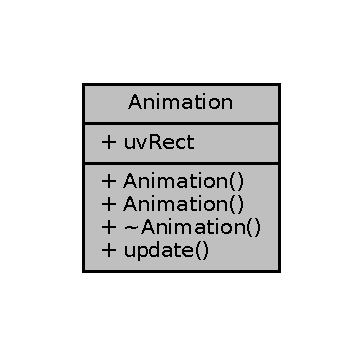
\includegraphics[width=174pt]{classAnimation__coll__graph}
\end{center}
\end{figure}
\subsection*{Public Member Functions}
\begin{DoxyCompactItemize}
\item 
\mbox{\hyperlink{classAnimation_a4c733083ff6e7c04ad06d73b5ccef398}{Animation}} ()=delete
\item 
\mbox{\hyperlink{classAnimation_aa8aaf286b114298e3ecbe1fc62572c27}{Animation}} (sf\+::\+Sprite \&texture, sf\+::\+Vector2u image\+Count, float switch\+Time)
\begin{DoxyCompactList}\small\item\em \mbox{\hyperlink{classAnimation}{Animation}} constructor. \end{DoxyCompactList}\item 
\mbox{\hyperlink{classAnimation_a401b68793d4fbf48d481c030ee4b2a16}{$\sim$\+Animation}} ()
\item 
void \mbox{\hyperlink{classAnimation_af09462caccc4d41ebfe288f703c4facd}{update}} (int row, float delta\+Time, bool face\+Right)
\begin{DoxyCompactList}\small\item\em Updates the character animation. \end{DoxyCompactList}\end{DoxyCompactItemize}
\subsection*{Public Attributes}
\begin{DoxyCompactItemize}
\item 
sf\+::\+Int\+Rect \mbox{\hyperlink{classAnimation_a82c41dd15d9a98ecc0699ecca09fd056}{uv\+Rect}}
\end{DoxyCompactItemize}


\subsection{Detailed Description}
\mbox{\hyperlink{classAnimation}{Animation}} class for the update of pixels, the class receive pictures of spritesheets and manages the cordinates at the sheet for other classes to be able to update 

\subsection{Constructor \& Destructor Documentation}
\mbox{\Hypertarget{classAnimation_a4c733083ff6e7c04ad06d73b5ccef398}\label{classAnimation_a4c733083ff6e7c04ad06d73b5ccef398}} 
\index{Animation@{Animation}!Animation@{Animation}}
\index{Animation@{Animation}!Animation@{Animation}}
\subsubsection{\texorpdfstring{Animation()}{Animation()}\hspace{0.1cm}{\footnotesize\ttfamily [1/2]}}
{\footnotesize\ttfamily Animation\+::\+Animation (\begin{DoxyParamCaption}{ }\end{DoxyParamCaption})\hspace{0.3cm}{\ttfamily [delete]}}

\mbox{\Hypertarget{classAnimation_aa8aaf286b114298e3ecbe1fc62572c27}\label{classAnimation_aa8aaf286b114298e3ecbe1fc62572c27}} 
\index{Animation@{Animation}!Animation@{Animation}}
\index{Animation@{Animation}!Animation@{Animation}}
\subsubsection{\texorpdfstring{Animation()}{Animation()}\hspace{0.1cm}{\footnotesize\ttfamily [2/2]}}
{\footnotesize\ttfamily Animation\+::\+Animation (\begin{DoxyParamCaption}\item[{sf\+::\+Sprite \&}]{texture,  }\item[{sf\+::\+Vector2u}]{image\+Count,  }\item[{float}]{switch\+Time }\end{DoxyParamCaption})}



\mbox{\hyperlink{classAnimation}{Animation}} constructor. 


\begin{DoxyParams}{Parameters}
{\em texture} & Texture sheet. \\
\hline
{\em image\+Count} & Image count of the texture sheet in the X axis \\
\hline
{\em switch\+Time} & Switch time for every sheet frame. \\
\hline
\end{DoxyParams}
\mbox{\Hypertarget{classAnimation_a401b68793d4fbf48d481c030ee4b2a16}\label{classAnimation_a401b68793d4fbf48d481c030ee4b2a16}} 
\index{Animation@{Animation}!````~Animation@{$\sim$\+Animation}}
\index{````~Animation@{$\sim$\+Animation}!Animation@{Animation}}
\subsubsection{\texorpdfstring{$\sim$\+Animation()}{~Animation()}}
{\footnotesize\ttfamily Animation\+::$\sim$\+Animation (\begin{DoxyParamCaption}{ }\end{DoxyParamCaption})}



\subsection{Member Function Documentation}
\mbox{\Hypertarget{classAnimation_af09462caccc4d41ebfe288f703c4facd}\label{classAnimation_af09462caccc4d41ebfe288f703c4facd}} 
\index{Animation@{Animation}!update@{update}}
\index{update@{update}!Animation@{Animation}}
\subsubsection{\texorpdfstring{update()}{update()}}
{\footnotesize\ttfamily void Animation\+::update (\begin{DoxyParamCaption}\item[{int}]{row,  }\item[{float}]{delta\+Time,  }\item[{bool}]{face\+Right }\end{DoxyParamCaption})}



Updates the character animation. 


\begin{DoxyParams}{Parameters}
{\em row} & Number of rows in the texture sheet. \\
\hline
{\em delta\+Time} & Pace time of the game. \\
\hline
{\em face\+Right} & Checks if the player is facing right or left \\
\hline
\end{DoxyParams}
Here is the caller graph for this function\+:\nopagebreak
\begin{figure}[H]
\begin{center}
\leavevmode
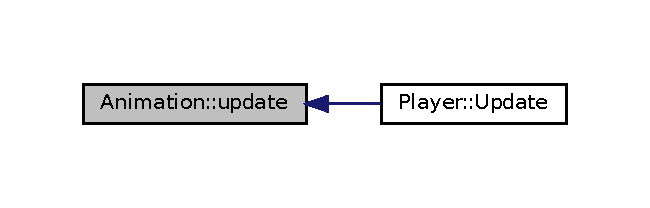
\includegraphics[width=312pt]{classAnimation_af09462caccc4d41ebfe288f703c4facd_icgraph}
\end{center}
\end{figure}


\subsection{Member Data Documentation}
\mbox{\Hypertarget{classAnimation_a82c41dd15d9a98ecc0699ecca09fd056}\label{classAnimation_a82c41dd15d9a98ecc0699ecca09fd056}} 
\index{Animation@{Animation}!uv\+Rect@{uv\+Rect}}
\index{uv\+Rect@{uv\+Rect}!Animation@{Animation}}
\subsubsection{\texorpdfstring{uv\+Rect}{uvRect}}
{\footnotesize\ttfamily sf\+::\+Int\+Rect Animation\+::uv\+Rect}



The documentation for this class was generated from the following files\+:\begin{DoxyCompactItemize}
\item 
\mbox{\hyperlink{Animation_8h}{Animation.\+h}}\item 
\mbox{\hyperlink{Animation_8cpp}{Animation.\+cpp}}\end{DoxyCompactItemize}

\hypertarget{classAssetManager}{}\section{Asset\+Manager Class Reference}
\label{classAssetManager}\index{Asset\+Manager@{Asset\+Manager}}


{\ttfamily \#include $<$Asset\+Manager.\+h$>$}



Collaboration diagram for Asset\+Manager\+:\nopagebreak
\begin{figure}[H]
\begin{center}
\leavevmode
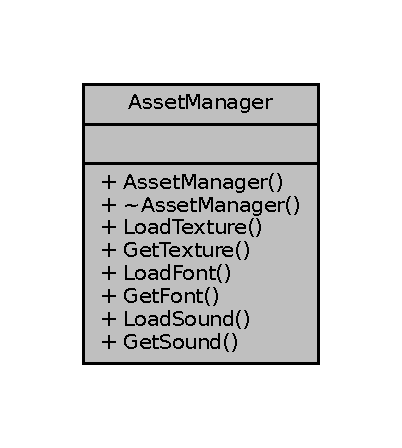
\includegraphics[width=193pt]{classAssetManager__coll__graph}
\end{center}
\end{figure}
\subsection*{Public Member Functions}
\begin{DoxyCompactItemize}
\item 
\mbox{\hyperlink{classAssetManager_a750ae7b39b633fbb6594443aa3ca704b}{Asset\+Manager}} ()
\item 
\mbox{\hyperlink{classAssetManager_a9c89817cbf3516f1451c116e89f47d30}{$\sim$\+Asset\+Manager}} ()
\item 
void \mbox{\hyperlink{classAssetManager_ada0c8171d6f0224c261080c04d954538}{Load\+Texture}} (std\+::string name, std\+::string file\+Name)
\begin{DoxyCompactList}\small\item\em Load Tetures. \end{DoxyCompactList}\item 
sf\+::\+Texture \& \mbox{\hyperlink{classAssetManager_aa72940e5dfecd91ff8c5a46ff0b4dfea}{Get\+Texture}} (std\+::string name)
\item 
void \mbox{\hyperlink{classAssetManager_a117f5cea9212e486210fb06dca8aa15a}{Load\+Font}} (std\+::string name, std\+::string file\+Name)
\begin{DoxyCompactList}\small\item\em Load Tetures. \end{DoxyCompactList}\item 
sf\+::\+Font \& \mbox{\hyperlink{classAssetManager_ac098205eb77fec60842b439215bf4c4f}{Get\+Font}} (std\+::string name)
\item 
void \mbox{\hyperlink{classAssetManager_a057918a0150c70d7c3c4eb72e7531ec7}{Load\+Sound}} (std\+::string name, std\+::string file\+Name)
\begin{DoxyCompactList}\small\item\em Load Tetures. \end{DoxyCompactList}\item 
sf\+::\+Sound\+Buffer \& \mbox{\hyperlink{classAssetManager_ad2a21b7f91975c3b74fd4c2c897d4601}{Get\+Sound}} (std\+::string name)
\end{DoxyCompactItemize}


\subsection{Detailed Description}
Assets Manager class is the class that stores all kind of resources needed for the game. 

\subsection{Constructor \& Destructor Documentation}
\mbox{\Hypertarget{classAssetManager_a750ae7b39b633fbb6594443aa3ca704b}\label{classAssetManager_a750ae7b39b633fbb6594443aa3ca704b}} 
\index{Asset\+Manager@{Asset\+Manager}!Asset\+Manager@{Asset\+Manager}}
\index{Asset\+Manager@{Asset\+Manager}!Asset\+Manager@{Asset\+Manager}}
\subsubsection{\texorpdfstring{Asset\+Manager()}{AssetManager()}}
{\footnotesize\ttfamily Asset\+Manager\+::\+Asset\+Manager (\begin{DoxyParamCaption}{ }\end{DoxyParamCaption})}

\mbox{\Hypertarget{classAssetManager_a9c89817cbf3516f1451c116e89f47d30}\label{classAssetManager_a9c89817cbf3516f1451c116e89f47d30}} 
\index{Asset\+Manager@{Asset\+Manager}!````~Asset\+Manager@{$\sim$\+Asset\+Manager}}
\index{````~Asset\+Manager@{$\sim$\+Asset\+Manager}!Asset\+Manager@{Asset\+Manager}}
\subsubsection{\texorpdfstring{$\sim$\+Asset\+Manager()}{~AssetManager()}}
{\footnotesize\ttfamily Asset\+Manager\+::$\sim$\+Asset\+Manager (\begin{DoxyParamCaption}{ }\end{DoxyParamCaption})}



\subsection{Member Function Documentation}
\mbox{\Hypertarget{classAssetManager_ac098205eb77fec60842b439215bf4c4f}\label{classAssetManager_ac098205eb77fec60842b439215bf4c4f}} 
\index{Asset\+Manager@{Asset\+Manager}!Get\+Font@{Get\+Font}}
\index{Get\+Font@{Get\+Font}!Asset\+Manager@{Asset\+Manager}}
\subsubsection{\texorpdfstring{Get\+Font()}{GetFont()}}
{\footnotesize\ttfamily sf\+::\+Font \& Asset\+Manager\+::\+Get\+Font (\begin{DoxyParamCaption}\item[{std\+::string}]{name }\end{DoxyParamCaption})}

\mbox{\Hypertarget{classAssetManager_ad2a21b7f91975c3b74fd4c2c897d4601}\label{classAssetManager_ad2a21b7f91975c3b74fd4c2c897d4601}} 
\index{Asset\+Manager@{Asset\+Manager}!Get\+Sound@{Get\+Sound}}
\index{Get\+Sound@{Get\+Sound}!Asset\+Manager@{Asset\+Manager}}
\subsubsection{\texorpdfstring{Get\+Sound()}{GetSound()}}
{\footnotesize\ttfamily sf\+::\+Sound\+Buffer \& Asset\+Manager\+::\+Get\+Sound (\begin{DoxyParamCaption}\item[{std\+::string}]{name }\end{DoxyParamCaption})}

\mbox{\Hypertarget{classAssetManager_aa72940e5dfecd91ff8c5a46ff0b4dfea}\label{classAssetManager_aa72940e5dfecd91ff8c5a46ff0b4dfea}} 
\index{Asset\+Manager@{Asset\+Manager}!Get\+Texture@{Get\+Texture}}
\index{Get\+Texture@{Get\+Texture}!Asset\+Manager@{Asset\+Manager}}
\subsubsection{\texorpdfstring{Get\+Texture()}{GetTexture()}}
{\footnotesize\ttfamily sf\+::\+Texture \& Asset\+Manager\+::\+Get\+Texture (\begin{DoxyParamCaption}\item[{std\+::string}]{name }\end{DoxyParamCaption})}

\mbox{\Hypertarget{classAssetManager_a117f5cea9212e486210fb06dca8aa15a}\label{classAssetManager_a117f5cea9212e486210fb06dca8aa15a}} 
\index{Asset\+Manager@{Asset\+Manager}!Load\+Font@{Load\+Font}}
\index{Load\+Font@{Load\+Font}!Asset\+Manager@{Asset\+Manager}}
\subsubsection{\texorpdfstring{Load\+Font()}{LoadFont()}}
{\footnotesize\ttfamily void Asset\+Manager\+::\+Load\+Font (\begin{DoxyParamCaption}\item[{std\+::string}]{name,  }\item[{std\+::string}]{file\+Name }\end{DoxyParamCaption})}



Load Tetures. 


\begin{DoxyParams}{Parameters}
{\em name} & Name of the font for the map storage. \\
\hline
{\em file\+Name} & Name of the font file. \\
\hline
\end{DoxyParams}
\mbox{\Hypertarget{classAssetManager_a057918a0150c70d7c3c4eb72e7531ec7}\label{classAssetManager_a057918a0150c70d7c3c4eb72e7531ec7}} 
\index{Asset\+Manager@{Asset\+Manager}!Load\+Sound@{Load\+Sound}}
\index{Load\+Sound@{Load\+Sound}!Asset\+Manager@{Asset\+Manager}}
\subsubsection{\texorpdfstring{Load\+Sound()}{LoadSound()}}
{\footnotesize\ttfamily void Asset\+Manager\+::\+Load\+Sound (\begin{DoxyParamCaption}\item[{std\+::string}]{name,  }\item[{std\+::string}]{file\+Name }\end{DoxyParamCaption})}



Load Tetures. 


\begin{DoxyParams}{Parameters}
{\em name} & Name of the sound for the map storage. \\
\hline
{\em file\+Name} & Name of the sound file. \\
\hline
\end{DoxyParams}
\mbox{\Hypertarget{classAssetManager_ada0c8171d6f0224c261080c04d954538}\label{classAssetManager_ada0c8171d6f0224c261080c04d954538}} 
\index{Asset\+Manager@{Asset\+Manager}!Load\+Texture@{Load\+Texture}}
\index{Load\+Texture@{Load\+Texture}!Asset\+Manager@{Asset\+Manager}}
\subsubsection{\texorpdfstring{Load\+Texture()}{LoadTexture()}}
{\footnotesize\ttfamily void Asset\+Manager\+::\+Load\+Texture (\begin{DoxyParamCaption}\item[{std\+::string}]{name,  }\item[{std\+::string}]{file\+Name }\end{DoxyParamCaption})}



Load Tetures. 


\begin{DoxyParams}{Parameters}
{\em name} & Name of the texture for the map storage. \\
\hline
{\em file\+Name} & Name of the texture file. \\
\hline
\end{DoxyParams}


The documentation for this class was generated from the following files\+:\begin{DoxyCompactItemize}
\item 
\mbox{\hyperlink{AssetManager_8h}{Asset\+Manager.\+h}}\item 
\mbox{\hyperlink{AssetManager_8cpp}{Asset\+Manager.\+cpp}}\end{DoxyCompactItemize}

\hypertarget{classGame}{}\section{Game Class Reference}
\label{classGame}\index{Game@{Game}}


{\ttfamily \#include $<$Game.\+h$>$}



Collaboration diagram for Game\+:\nopagebreak
\begin{figure}[H]
\begin{center}
\leavevmode
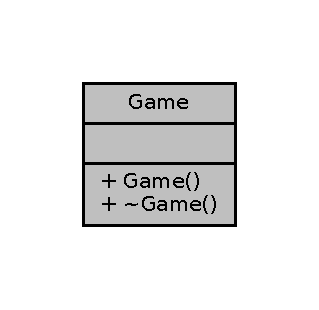
\includegraphics[width=153pt]{classGame__coll__graph}
\end{center}
\end{figure}
\subsection*{Public Member Functions}
\begin{DoxyCompactItemize}
\item 
\mbox{\hyperlink{classGame_a0688bdc6486839d4436175d1d05773e0}{Game}} (int width, int height, std\+::string title)
\item 
\mbox{\hyperlink{classGame_ae3d112ca6e0e55150d2fdbc704474530}{$\sim$\+Game}} ()
\end{DoxyCompactItemize}


\subsection{Constructor \& Destructor Documentation}
\mbox{\Hypertarget{classGame_a0688bdc6486839d4436175d1d05773e0}\label{classGame_a0688bdc6486839d4436175d1d05773e0}} 
\index{Game@{Game}!Game@{Game}}
\index{Game@{Game}!Game@{Game}}
\subsubsection{\texorpdfstring{Game()}{Game()}}
{\footnotesize\ttfamily Game\+::\+Game (\begin{DoxyParamCaption}\item[{int}]{width,  }\item[{int}]{height,  }\item[{std\+::string}]{title }\end{DoxyParamCaption})}

\mbox{\Hypertarget{classGame_ae3d112ca6e0e55150d2fdbc704474530}\label{classGame_ae3d112ca6e0e55150d2fdbc704474530}} 
\index{Game@{Game}!````~Game@{$\sim$\+Game}}
\index{````~Game@{$\sim$\+Game}!Game@{Game}}
\subsubsection{\texorpdfstring{$\sim$\+Game()}{~Game()}}
{\footnotesize\ttfamily Game\+::$\sim$\+Game (\begin{DoxyParamCaption}{ }\end{DoxyParamCaption})}



The documentation for this class was generated from the following files\+:\begin{DoxyCompactItemize}
\item 
\mbox{\hyperlink{Game_8h}{Game.\+h}}\item 
\mbox{\hyperlink{Game_8cpp}{Game.\+cpp}}\end{DoxyCompactItemize}

\hypertarget{structGameData}{}\section{Game\+Data Struct Reference}
\label{structGameData}\index{Game\+Data@{Game\+Data}}


{\ttfamily \#include $<$Game.\+h$>$}



Collaboration diagram for Game\+Data\+:
\nopagebreak
\begin{figure}[H]
\begin{center}
\leavevmode
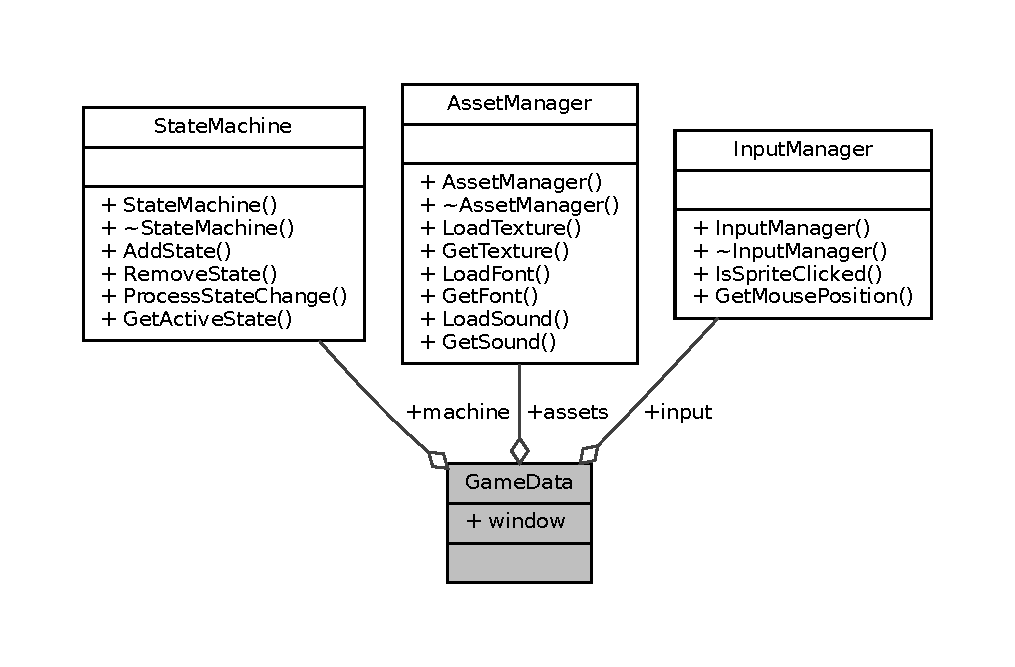
\includegraphics[width=350pt]{structGameData__coll__graph}
\end{center}
\end{figure}
\subsection*{Public Attributes}
\begin{DoxyCompactItemize}
\item 
\mbox{\hyperlink{classStateMachine}{State\+Machine}} \mbox{\hyperlink{structGameData_a8dfa448b18baef58877cd0365f4c1978}{machine}}
\item 
sf\+::\+Render\+Window \mbox{\hyperlink{structGameData_ad3ebf49a95d78b14047b92b20d39b810}{window}}
\item 
\mbox{\hyperlink{classAssetManager}{Asset\+Manager}} \mbox{\hyperlink{structGameData_ad19b66c159b0f14aecb7b2fd92d1b7bb}{assets}}
\item 
\mbox{\hyperlink{classInputManager}{Input\+Manager}} \mbox{\hyperlink{structGameData_abdfb34b80f7627eebbe484144dd9b589}{input}}
\end{DoxyCompactItemize}


\subsection{Member Data Documentation}
\mbox{\Hypertarget{structGameData_ad19b66c159b0f14aecb7b2fd92d1b7bb}\label{structGameData_ad19b66c159b0f14aecb7b2fd92d1b7bb}} 
\index{Game\+Data@{Game\+Data}!assets@{assets}}
\index{assets@{assets}!Game\+Data@{Game\+Data}}
\subsubsection{\texorpdfstring{assets}{assets}}
{\footnotesize\ttfamily \mbox{\hyperlink{classAssetManager}{Asset\+Manager}} Game\+Data\+::assets}

\mbox{\Hypertarget{structGameData_abdfb34b80f7627eebbe484144dd9b589}\label{structGameData_abdfb34b80f7627eebbe484144dd9b589}} 
\index{Game\+Data@{Game\+Data}!input@{input}}
\index{input@{input}!Game\+Data@{Game\+Data}}
\subsubsection{\texorpdfstring{input}{input}}
{\footnotesize\ttfamily \mbox{\hyperlink{classInputManager}{Input\+Manager}} Game\+Data\+::input}

\mbox{\Hypertarget{structGameData_a8dfa448b18baef58877cd0365f4c1978}\label{structGameData_a8dfa448b18baef58877cd0365f4c1978}} 
\index{Game\+Data@{Game\+Data}!machine@{machine}}
\index{machine@{machine}!Game\+Data@{Game\+Data}}
\subsubsection{\texorpdfstring{machine}{machine}}
{\footnotesize\ttfamily \mbox{\hyperlink{classStateMachine}{State\+Machine}} Game\+Data\+::machine}

\mbox{\Hypertarget{structGameData_ad3ebf49a95d78b14047b92b20d39b810}\label{structGameData_ad3ebf49a95d78b14047b92b20d39b810}} 
\index{Game\+Data@{Game\+Data}!window@{window}}
\index{window@{window}!Game\+Data@{Game\+Data}}
\subsubsection{\texorpdfstring{window}{window}}
{\footnotesize\ttfamily sf\+::\+Render\+Window Game\+Data\+::window}



The documentation for this struct was generated from the following file\+:\begin{DoxyCompactItemize}
\item 
\mbox{\hyperlink{Game_8h}{Game.\+h}}\end{DoxyCompactItemize}

\hypertarget{classGameOver}{}\section{Game\+Over Class Reference}
\label{classGameOver}\index{Game\+Over@{Game\+Over}}


{\ttfamily \#include $<$Game\+Over.\+h$>$}



Inheritance diagram for Game\+Over\+:\nopagebreak
\begin{figure}[H]
\begin{center}
\leavevmode
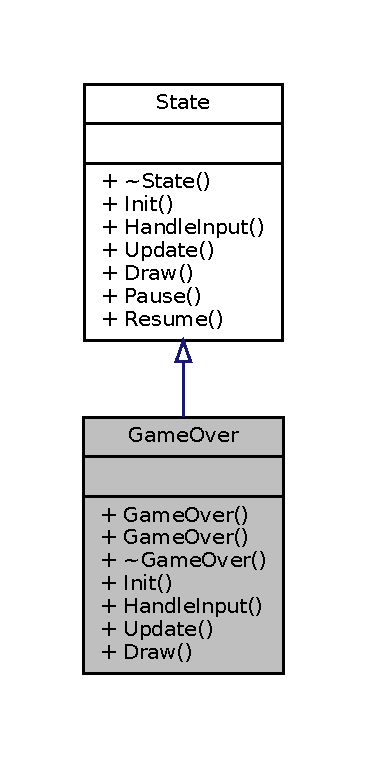
\includegraphics[width=176pt]{classGameOver__inherit__graph}
\end{center}
\end{figure}


Collaboration diagram for Game\+Over\+:\nopagebreak
\begin{figure}[H]
\begin{center}
\leavevmode
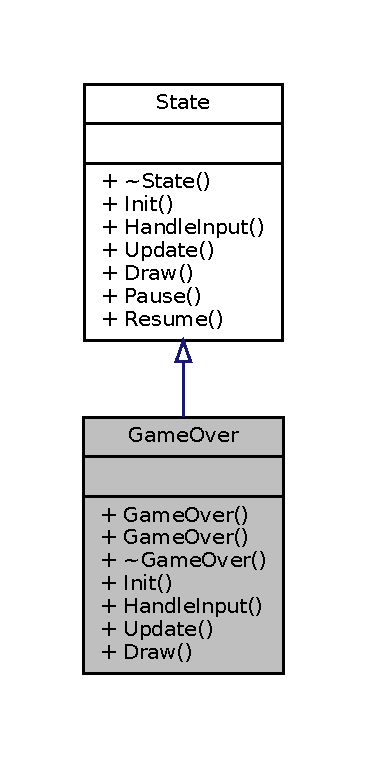
\includegraphics[width=176pt]{classGameOver__coll__graph}
\end{center}
\end{figure}
\subsection*{Public Member Functions}
\begin{DoxyCompactItemize}
\item 
\mbox{\hyperlink{classGameOver_a191161f50e27feba1a5fd18aa867fbf2}{Game\+Over}} ()=delete
\item 
\mbox{\hyperlink{classGameOver_a2ed53e8b1c1fe4e8e73d88fbb548da5a}{Game\+Over}} (\mbox{\hyperlink{Game_8h_aff850703a7797c8bfee2f02906aec50c}{Game\+Data\+Ref}} data)
\item 
\mbox{\hyperlink{classGameOver_ae36951a153d25d52fab7cbc7a85bbbbd}{$\sim$\+Game\+Over}} ()
\item 
void \mbox{\hyperlink{classGameOver_ac13d1bd0fe9f8db0ef0301c9ec63a9e0}{Init}} ()
\item 
void \mbox{\hyperlink{classGameOver_a1b90d0ed04386fe166cbfcf2427a5175}{Handle\+Input}} ()
\item 
void \mbox{\hyperlink{classGameOver_a960c8ff2705f1fe49b49c717ee68fbc6}{Update}} (float delta\+Time)
\item 
void \mbox{\hyperlink{classGameOver_a263a49026ce81b22721cfc515f8efd4e}{Draw}} (float delta\+Time)
\end{DoxyCompactItemize}


\subsection{Constructor \& Destructor Documentation}
\mbox{\Hypertarget{classGameOver_a191161f50e27feba1a5fd18aa867fbf2}\label{classGameOver_a191161f50e27feba1a5fd18aa867fbf2}} 
\index{Game\+Over@{Game\+Over}!Game\+Over@{Game\+Over}}
\index{Game\+Over@{Game\+Over}!Game\+Over@{Game\+Over}}
\subsubsection{\texorpdfstring{Game\+Over()}{GameOver()}\hspace{0.1cm}{\footnotesize\ttfamily [1/2]}}
{\footnotesize\ttfamily Game\+Over\+::\+Game\+Over (\begin{DoxyParamCaption}{ }\end{DoxyParamCaption})\hspace{0.3cm}{\ttfamily [delete]}}

\mbox{\Hypertarget{classGameOver_a2ed53e8b1c1fe4e8e73d88fbb548da5a}\label{classGameOver_a2ed53e8b1c1fe4e8e73d88fbb548da5a}} 
\index{Game\+Over@{Game\+Over}!Game\+Over@{Game\+Over}}
\index{Game\+Over@{Game\+Over}!Game\+Over@{Game\+Over}}
\subsubsection{\texorpdfstring{Game\+Over()}{GameOver()}\hspace{0.1cm}{\footnotesize\ttfamily [2/2]}}
{\footnotesize\ttfamily Game\+Over\+::\+Game\+Over (\begin{DoxyParamCaption}\item[{\mbox{\hyperlink{Game_8h_aff850703a7797c8bfee2f02906aec50c}{Game\+Data\+Ref}}}]{data }\end{DoxyParamCaption})}

\mbox{\Hypertarget{classGameOver_ae36951a153d25d52fab7cbc7a85bbbbd}\label{classGameOver_ae36951a153d25d52fab7cbc7a85bbbbd}} 
\index{Game\+Over@{Game\+Over}!````~Game\+Over@{$\sim$\+Game\+Over}}
\index{````~Game\+Over@{$\sim$\+Game\+Over}!Game\+Over@{Game\+Over}}
\subsubsection{\texorpdfstring{$\sim$\+Game\+Over()}{~GameOver()}}
{\footnotesize\ttfamily Game\+Over\+::$\sim$\+Game\+Over (\begin{DoxyParamCaption}{ }\end{DoxyParamCaption})}



\subsection{Member Function Documentation}
\mbox{\Hypertarget{classGameOver_a263a49026ce81b22721cfc515f8efd4e}\label{classGameOver_a263a49026ce81b22721cfc515f8efd4e}} 
\index{Game\+Over@{Game\+Over}!Draw@{Draw}}
\index{Draw@{Draw}!Game\+Over@{Game\+Over}}
\subsubsection{\texorpdfstring{Draw()}{Draw()}}
{\footnotesize\ttfamily void Game\+Over\+::\+Draw (\begin{DoxyParamCaption}\item[{float}]{delta\+Time }\end{DoxyParamCaption})\hspace{0.3cm}{\ttfamily [virtual]}}



Implements \mbox{\hyperlink{classState_ae3bc988c6103665bca68560742fb40e1}{State}}.

\mbox{\Hypertarget{classGameOver_a1b90d0ed04386fe166cbfcf2427a5175}\label{classGameOver_a1b90d0ed04386fe166cbfcf2427a5175}} 
\index{Game\+Over@{Game\+Over}!Handle\+Input@{Handle\+Input}}
\index{Handle\+Input@{Handle\+Input}!Game\+Over@{Game\+Over}}
\subsubsection{\texorpdfstring{Handle\+Input()}{HandleInput()}}
{\footnotesize\ttfamily void Game\+Over\+::\+Handle\+Input (\begin{DoxyParamCaption}{ }\end{DoxyParamCaption})\hspace{0.3cm}{\ttfamily [virtual]}}



Implements \mbox{\hyperlink{classState_ad3de659bdeb45c97486464461d625e8f}{State}}.

\mbox{\Hypertarget{classGameOver_ac13d1bd0fe9f8db0ef0301c9ec63a9e0}\label{classGameOver_ac13d1bd0fe9f8db0ef0301c9ec63a9e0}} 
\index{Game\+Over@{Game\+Over}!Init@{Init}}
\index{Init@{Init}!Game\+Over@{Game\+Over}}
\subsubsection{\texorpdfstring{Init()}{Init()}}
{\footnotesize\ttfamily void Game\+Over\+::\+Init (\begin{DoxyParamCaption}{ }\end{DoxyParamCaption})\hspace{0.3cm}{\ttfamily [virtual]}}



Implements \mbox{\hyperlink{classState_a7ab4d8c6aa239a17ed579d89a209b156}{State}}.

\mbox{\Hypertarget{classGameOver_a960c8ff2705f1fe49b49c717ee68fbc6}\label{classGameOver_a960c8ff2705f1fe49b49c717ee68fbc6}} 
\index{Game\+Over@{Game\+Over}!Update@{Update}}
\index{Update@{Update}!Game\+Over@{Game\+Over}}
\subsubsection{\texorpdfstring{Update()}{Update()}}
{\footnotesize\ttfamily void Game\+Over\+::\+Update (\begin{DoxyParamCaption}\item[{float}]{delta\+Time }\end{DoxyParamCaption})\hspace{0.3cm}{\ttfamily [virtual]}}



Implements \mbox{\hyperlink{classState_a770f40188fdfc64bc95a5166fef12e02}{State}}.



The documentation for this class was generated from the following files\+:\begin{DoxyCompactItemize}
\item 
\mbox{\hyperlink{GameOver_8h}{Game\+Over.\+h}}\item 
\mbox{\hyperlink{GameOver_8cpp}{Game\+Over.\+cpp}}\end{DoxyCompactItemize}

\hypertarget{classInputManager}{}\section{Input\+Manager Class Reference}
\label{classInputManager}\index{Input\+Manager@{Input\+Manager}}


Gets mouse button Inputs.  




{\ttfamily \#include $<$Input\+Manager.\+h$>$}



Collaboration diagram for Input\+Manager\+:\nopagebreak
\begin{figure}[H]
\begin{center}
\leavevmode
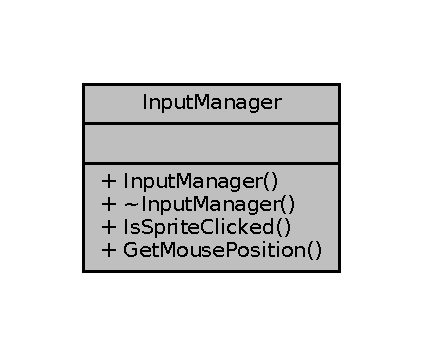
\includegraphics[width=203pt]{classInputManager__coll__graph}
\end{center}
\end{figure}
\subsection*{Public Member Functions}
\begin{DoxyCompactItemize}
\item 
\mbox{\hyperlink{classInputManager_a8be46886da639b26d67181c29dab6d6c}{Input\+Manager}} ()
\item 
\mbox{\hyperlink{classInputManager_af518290877dd183606709d5852db5491}{$\sim$\+Input\+Manager}} ()
\item 
bool \mbox{\hyperlink{classInputManager_a39886282f4c7871f3892f6ed16a545d3}{Is\+Sprite\+Clicked}} (sf\+::\+Sprite object, sf\+::\+Mouse\+::\+Button, sf\+::\+Render\+Window \&window)
\begin{DoxyCompactList}\small\item\em Checks if a specific sprite have been clicked. \end{DoxyCompactList}\item 
sf\+::\+Vector2i \mbox{\hyperlink{classInputManager_a4c9492c2d988fae3b5f5e21eab7ba72d}{Get\+Mouse\+Position}} (sf\+::\+Render\+Window \&window)
\begin{DoxyCompactList}\small\item\em Returns the mouse position in the screen. \end{DoxyCompactList}\end{DoxyCompactItemize}


\subsection{Detailed Description}
Gets mouse button Inputs. 



\subsection{Constructor \& Destructor Documentation}
\mbox{\Hypertarget{classInputManager_a8be46886da639b26d67181c29dab6d6c}\label{classInputManager_a8be46886da639b26d67181c29dab6d6c}} 
\index{Input\+Manager@{Input\+Manager}!Input\+Manager@{Input\+Manager}}
\index{Input\+Manager@{Input\+Manager}!Input\+Manager@{Input\+Manager}}
\subsubsection{\texorpdfstring{Input\+Manager()}{InputManager()}}
{\footnotesize\ttfamily Input\+Manager\+::\+Input\+Manager (\begin{DoxyParamCaption}{ }\end{DoxyParamCaption})}

\mbox{\Hypertarget{classInputManager_af518290877dd183606709d5852db5491}\label{classInputManager_af518290877dd183606709d5852db5491}} 
\index{Input\+Manager@{Input\+Manager}!````~Input\+Manager@{$\sim$\+Input\+Manager}}
\index{````~Input\+Manager@{$\sim$\+Input\+Manager}!Input\+Manager@{Input\+Manager}}
\subsubsection{\texorpdfstring{$\sim$\+Input\+Manager()}{~InputManager()}}
{\footnotesize\ttfamily Input\+Manager\+::$\sim$\+Input\+Manager (\begin{DoxyParamCaption}{ }\end{DoxyParamCaption})}



\subsection{Member Function Documentation}
\mbox{\Hypertarget{classInputManager_a4c9492c2d988fae3b5f5e21eab7ba72d}\label{classInputManager_a4c9492c2d988fae3b5f5e21eab7ba72d}} 
\index{Input\+Manager@{Input\+Manager}!Get\+Mouse\+Position@{Get\+Mouse\+Position}}
\index{Get\+Mouse\+Position@{Get\+Mouse\+Position}!Input\+Manager@{Input\+Manager}}
\subsubsection{\texorpdfstring{Get\+Mouse\+Position()}{GetMousePosition()}}
{\footnotesize\ttfamily sf\+::\+Vector2i Input\+Manager\+::\+Get\+Mouse\+Position (\begin{DoxyParamCaption}\item[{sf\+::\+Render\+Window \&}]{window }\end{DoxyParamCaption})}



Returns the mouse position in the screen. 


\begin{DoxyParams}{Parameters}
{\em window} & \mbox{\hyperlink{classGame}{Game}} window. \\
\hline
\end{DoxyParams}
\mbox{\Hypertarget{classInputManager_a39886282f4c7871f3892f6ed16a545d3}\label{classInputManager_a39886282f4c7871f3892f6ed16a545d3}} 
\index{Input\+Manager@{Input\+Manager}!Is\+Sprite\+Clicked@{Is\+Sprite\+Clicked}}
\index{Is\+Sprite\+Clicked@{Is\+Sprite\+Clicked}!Input\+Manager@{Input\+Manager}}
\subsubsection{\texorpdfstring{Is\+Sprite\+Clicked()}{IsSpriteClicked()}}
{\footnotesize\ttfamily bool Input\+Manager\+::\+Is\+Sprite\+Clicked (\begin{DoxyParamCaption}\item[{sf\+::\+Sprite}]{object,  }\item[{sf\+::\+Mouse\+::\+Button}]{button,  }\item[{sf\+::\+Render\+Window \&}]{window }\end{DoxyParamCaption})}



Checks if a specific sprite have been clicked. 


\begin{DoxyParams}{Parameters}
{\em object} & Sprite to be clicked. \\
\hline
{\em Second\+Parameter} & wich button click \\
\hline
{\em window} & \mbox{\hyperlink{classGame}{Game}} window. \\
\hline
\end{DoxyParams}


The documentation for this class was generated from the following files\+:\begin{DoxyCompactItemize}
\item 
\mbox{\hyperlink{InputManager_8h}{Input\+Manager.\+h}}\item 
\mbox{\hyperlink{InputManager_8cpp}{Input\+Manager.\+cpp}}\end{DoxyCompactItemize}

\hypertarget{classIntroState}{}\section{Intro\+State Class Reference}
\label{classIntroState}\index{Intro\+State@{Intro\+State}}


{\ttfamily \#include $<$Intro\+State.\+h$>$}



Inheritance diagram for Intro\+State\+:\nopagebreak
\begin{figure}[H]
\begin{center}
\leavevmode
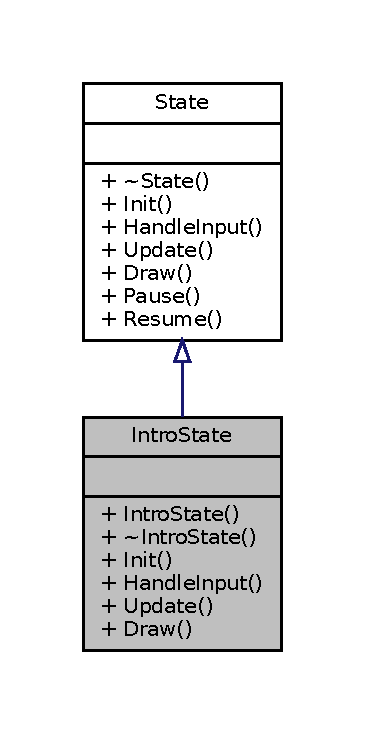
\includegraphics[width=175pt]{classIntroState__inherit__graph}
\end{center}
\end{figure}


Collaboration diagram for Intro\+State\+:\nopagebreak
\begin{figure}[H]
\begin{center}
\leavevmode
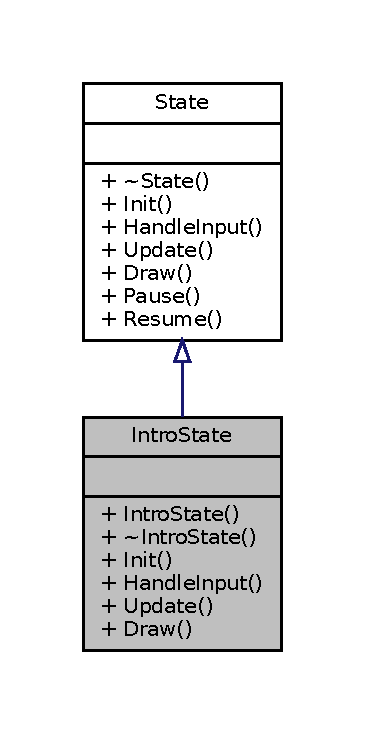
\includegraphics[width=175pt]{classIntroState__coll__graph}
\end{center}
\end{figure}
\subsection*{Public Member Functions}
\begin{DoxyCompactItemize}
\item 
\mbox{\hyperlink{classIntroState_ab4dc575c648c2589c7b110f5c930601c}{Intro\+State}} (\mbox{\hyperlink{Game_8h_aff850703a7797c8bfee2f02906aec50c}{Game\+Data\+Ref}} data)
\item 
\mbox{\hyperlink{classIntroState_a33fe62d2ddc9d079f716016674090b05}{$\sim$\+Intro\+State}} ()
\item 
void \mbox{\hyperlink{classIntroState_a065e914b336c162b1467845c7126c920}{Init}} ()
\item 
void \mbox{\hyperlink{classIntroState_a6a2a89b3374f53e1bcf366c0ae896109}{Handle\+Input}} ()
\item 
void \mbox{\hyperlink{classIntroState_a781891b1db3bdbf6af228ef85c0df00a}{Update}} (float delta\+Time)
\begin{DoxyCompactList}\small\item\em Updates the menu frames. \end{DoxyCompactList}\item 
void \mbox{\hyperlink{classIntroState_a903b8e2b781eae1e9a6e7db08d38fd2c}{Draw}} (float delta\+Time)
\begin{DoxyCompactList}\small\item\em Updates the menu frames. \end{DoxyCompactList}\end{DoxyCompactItemize}


\subsection{Detailed Description}
Introduction of the game, image for about 2 seconds. 

\subsection{Constructor \& Destructor Documentation}
\mbox{\Hypertarget{classIntroState_ab4dc575c648c2589c7b110f5c930601c}\label{classIntroState_ab4dc575c648c2589c7b110f5c930601c}} 
\index{Intro\+State@{Intro\+State}!Intro\+State@{Intro\+State}}
\index{Intro\+State@{Intro\+State}!Intro\+State@{Intro\+State}}
\subsubsection{\texorpdfstring{Intro\+State()}{IntroState()}}
{\footnotesize\ttfamily Intro\+State\+::\+Intro\+State (\begin{DoxyParamCaption}\item[{\mbox{\hyperlink{Game_8h_aff850703a7797c8bfee2f02906aec50c}{Game\+Data\+Ref}}}]{data }\end{DoxyParamCaption})}

\mbox{\Hypertarget{classIntroState_a33fe62d2ddc9d079f716016674090b05}\label{classIntroState_a33fe62d2ddc9d079f716016674090b05}} 
\index{Intro\+State@{Intro\+State}!````~Intro\+State@{$\sim$\+Intro\+State}}
\index{````~Intro\+State@{$\sim$\+Intro\+State}!Intro\+State@{Intro\+State}}
\subsubsection{\texorpdfstring{$\sim$\+Intro\+State()}{~IntroState()}}
{\footnotesize\ttfamily Intro\+State\+::$\sim$\+Intro\+State (\begin{DoxyParamCaption}{ }\end{DoxyParamCaption})}



\subsection{Member Function Documentation}
\mbox{\Hypertarget{classIntroState_a903b8e2b781eae1e9a6e7db08d38fd2c}\label{classIntroState_a903b8e2b781eae1e9a6e7db08d38fd2c}} 
\index{Intro\+State@{Intro\+State}!Draw@{Draw}}
\index{Draw@{Draw}!Intro\+State@{Intro\+State}}
\subsubsection{\texorpdfstring{Draw()}{Draw()}}
{\footnotesize\ttfamily void Intro\+State\+::\+Draw (\begin{DoxyParamCaption}\item[{float}]{delta\+Time }\end{DoxyParamCaption})\hspace{0.3cm}{\ttfamily [virtual]}}



Updates the menu frames. 


\begin{DoxyParams}{Parameters}
{\em delta\+Time} & Pace timing. \\
\hline
\end{DoxyParams}


Implements \mbox{\hyperlink{classState_ae3bc988c6103665bca68560742fb40e1}{State}}.

\mbox{\Hypertarget{classIntroState_a6a2a89b3374f53e1bcf366c0ae896109}\label{classIntroState_a6a2a89b3374f53e1bcf366c0ae896109}} 
\index{Intro\+State@{Intro\+State}!Handle\+Input@{Handle\+Input}}
\index{Handle\+Input@{Handle\+Input}!Intro\+State@{Intro\+State}}
\subsubsection{\texorpdfstring{Handle\+Input()}{HandleInput()}}
{\footnotesize\ttfamily void Intro\+State\+::\+Handle\+Input (\begin{DoxyParamCaption}{ }\end{DoxyParamCaption})\hspace{0.3cm}{\ttfamily [virtual]}}

Handles Input during this stage 

Implements \mbox{\hyperlink{classState_ad3de659bdeb45c97486464461d625e8f}{State}}.

\mbox{\Hypertarget{classIntroState_a065e914b336c162b1467845c7126c920}\label{classIntroState_a065e914b336c162b1467845c7126c920}} 
\index{Intro\+State@{Intro\+State}!Init@{Init}}
\index{Init@{Init}!Intro\+State@{Intro\+State}}
\subsubsection{\texorpdfstring{Init()}{Init()}}
{\footnotesize\ttfamily void Intro\+State\+::\+Init (\begin{DoxyParamCaption}{ }\end{DoxyParamCaption})\hspace{0.3cm}{\ttfamily [virtual]}}

Initializes needed engine parts needed. 

Implements \mbox{\hyperlink{classState_a7ab4d8c6aa239a17ed579d89a209b156}{State}}.

\mbox{\Hypertarget{classIntroState_a781891b1db3bdbf6af228ef85c0df00a}\label{classIntroState_a781891b1db3bdbf6af228ef85c0df00a}} 
\index{Intro\+State@{Intro\+State}!Update@{Update}}
\index{Update@{Update}!Intro\+State@{Intro\+State}}
\subsubsection{\texorpdfstring{Update()}{Update()}}
{\footnotesize\ttfamily void Intro\+State\+::\+Update (\begin{DoxyParamCaption}\item[{float}]{delta\+Time }\end{DoxyParamCaption})\hspace{0.3cm}{\ttfamily [virtual]}}



Updates the menu frames. 


\begin{DoxyParams}{Parameters}
{\em delta\+Time} & Pace timing. \\
\hline
\end{DoxyParams}


Implements \mbox{\hyperlink{classState_a770f40188fdfc64bc95a5166fef12e02}{State}}.



The documentation for this class was generated from the following files\+:\begin{DoxyCompactItemize}
\item 
\mbox{\hyperlink{IntroState_8h}{Intro\+State.\+h}}\item 
\mbox{\hyperlink{IntroState_8cpp}{Intro\+State.\+cpp}}\end{DoxyCompactItemize}

\hypertarget{classMap}{}\section{Map Class Reference}
\label{classMap}\index{Map@{Map}}


{\ttfamily \#include $<$Map.\+h$>$}



Collaboration diagram for Map\+:\nopagebreak
\begin{figure}[H]
\begin{center}
\leavevmode
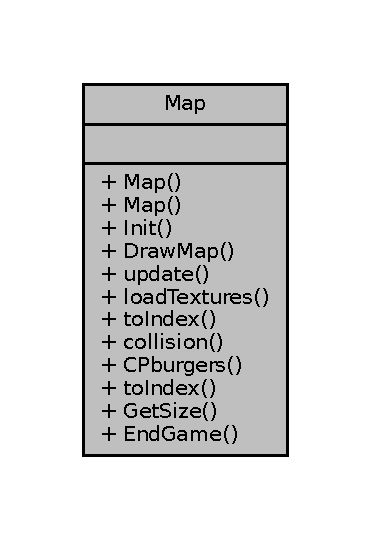
\includegraphics[width=178pt]{classMap__coll__graph}
\end{center}
\end{figure}
\subsection*{Public Member Functions}
\begin{DoxyCompactItemize}
\item 
\mbox{\hyperlink{classMap_a7c19436c39c47715bee04c9a2390ac27}{Map}} ()=delete
\item 
\mbox{\hyperlink{classMap_a09823ddb7b00abc80dc72a4583469c58}{Map}} (\mbox{\hyperlink{Game_8h_aff850703a7797c8bfee2f02906aec50c}{Game\+Data\+Ref}} data, int tile\+Width, int n\+TilesW, int n\+TilesH)
\begin{DoxyCompactList}\small\item\em Updates the menu frames. \end{DoxyCompactList}\item 
void \mbox{\hyperlink{classMap_a67b222c575eee96246c2f3fd25b4912c}{Init}} ()
\begin{DoxyCompactList}\small\item\em Initializes all the needed parts of the map. \end{DoxyCompactList}\item 
void \mbox{\hyperlink{classMap_a3d0c3cf82f949ab01c788ab1c3e7f799}{Draw\+Map}} (float delta\+Time)
\begin{DoxyCompactList}\small\item\em Updates the menu frames. \end{DoxyCompactList}\item 
void \mbox{\hyperlink{classMap_a7346023f96a36368daa2d4cafd4523f2}{update}} (float delta\+Time, sf\+::\+Render\+Window \&window)
\begin{DoxyCompactList}\small\item\em Updates the menu frames. \end{DoxyCompactList}\item 
void \mbox{\hyperlink{classMap_a63ecd67d43e63befe38de3e438abedff}{load\+Textures}} (std\+::string file\+Name)
\begin{DoxyCompactList}\small\item\em Updates the menu frames. \end{DoxyCompactList}\item 
int \mbox{\hyperlink{classMap_a378ff701ba69cfe800693466f8f3299e}{to\+Index}} (int x, int y)
\begin{DoxyCompactList}\small\item\em Transforms x and y intro the right the index of the tile map vector. \end{DoxyCompactList}\item 
void \mbox{\hyperlink{classMap_ae2311b25220590e05479d66408eeaabf}{collision}} ()
\begin{DoxyCompactList}\small\item\em Updates the player collision with the map. \end{DoxyCompactList}\item 
void \mbox{\hyperlink{classMap_a8485dce46ceae190bc9f51e22885eca3}{C\+Pburgers}} ()
\begin{DoxyCompactList}\small\item\em Spawn all the burgers based on the tile map. \end{DoxyCompactList}\item 
int \mbox{\hyperlink{classMap_a52f3ef46020dd2f6544fa2ee8dc9f4ff}{to\+Index}} (sf\+::\+Vector2i vec)
\begin{DoxyCompactList}\small\item\em Transforms a vector coordinate into the vector index och the tile map. \end{DoxyCompactList}\item 
sf\+::\+Vector2f \mbox{\hyperlink{classMap_a0c46c2c55236317c42854758b1af682f}{Get\+Size}} () const
\begin{DoxyCompactList}\small\item\em Get map size. \end{DoxyCompactList}\item 
void \mbox{\hyperlink{classMap_af58f98cfacd972d950201cc25df95982}{End\+Game}} ()
\begin{DoxyCompactList}\small\item\em Checks if the game has ended. \end{DoxyCompactList}\end{DoxyCompactItemize}
\subsection*{Friends}
\begin{DoxyCompactItemize}
\item 
class \mbox{\hyperlink{classMap_a8a97b6d5e408db103798551949a4e1f8}{Stage\+One}}
\end{DoxyCompactItemize}


\subsection{Detailed Description}
\mbox{\hyperlink{classMap}{Map}} class where the game levels will be created and with help of other classes create the game inviroment. 

\subsection{Constructor \& Destructor Documentation}
\mbox{\Hypertarget{classMap_a7c19436c39c47715bee04c9a2390ac27}\label{classMap_a7c19436c39c47715bee04c9a2390ac27}} 
\index{Map@{Map}!Map@{Map}}
\index{Map@{Map}!Map@{Map}}
\subsubsection{\texorpdfstring{Map()}{Map()}\hspace{0.1cm}{\footnotesize\ttfamily [1/2]}}
{\footnotesize\ttfamily Map\+::\+Map (\begin{DoxyParamCaption}{ }\end{DoxyParamCaption})\hspace{0.3cm}{\ttfamily [delete]}}

\mbox{\Hypertarget{classMap_a09823ddb7b00abc80dc72a4583469c58}\label{classMap_a09823ddb7b00abc80dc72a4583469c58}} 
\index{Map@{Map}!Map@{Map}}
\index{Map@{Map}!Map@{Map}}
\subsubsection{\texorpdfstring{Map()}{Map()}\hspace{0.1cm}{\footnotesize\ttfamily [2/2]}}
{\footnotesize\ttfamily Map\+::\+Map (\begin{DoxyParamCaption}\item[{\mbox{\hyperlink{Game_8h_aff850703a7797c8bfee2f02906aec50c}{Game\+Data\+Ref}}}]{data,  }\item[{int}]{tile\+Width,  }\item[{int}]{n\+TilesW,  }\item[{int}]{n\+TilesH }\end{DoxyParamCaption})}



Updates the menu frames. 


\begin{DoxyParams}{Parameters}
{\em data} & Variable that links all the engine parts to each other. \\
\hline
{\em tile\+Width} & \mbox{\hyperlink{structTile}{Tile}} size. \\
\hline
{\em n\+TilesW} & Width of the map. \\
\hline
{\em n\+TilesH} & Height of the map. \\
\hline
\end{DoxyParams}


\subsection{Member Function Documentation}
\mbox{\Hypertarget{classMap_ae2311b25220590e05479d66408eeaabf}\label{classMap_ae2311b25220590e05479d66408eeaabf}} 
\index{Map@{Map}!collision@{collision}}
\index{collision@{collision}!Map@{Map}}
\subsubsection{\texorpdfstring{collision()}{collision()}}
{\footnotesize\ttfamily void Map\+::collision (\begin{DoxyParamCaption}{ }\end{DoxyParamCaption})}



Updates the player collision with the map. 

Here is the call graph for this function\+:\nopagebreak
\begin{figure}[H]
\begin{center}
\leavevmode
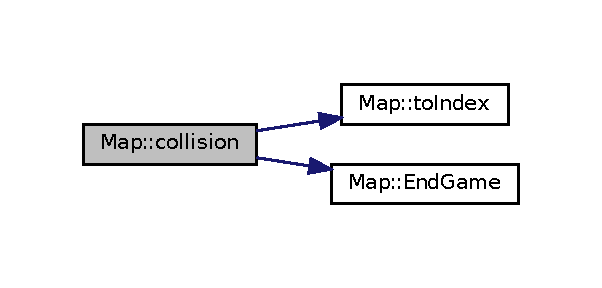
\includegraphics[width=289pt]{classMap_ae2311b25220590e05479d66408eeaabf_cgraph}
\end{center}
\end{figure}
Here is the caller graph for this function\+:\nopagebreak
\begin{figure}[H]
\begin{center}
\leavevmode
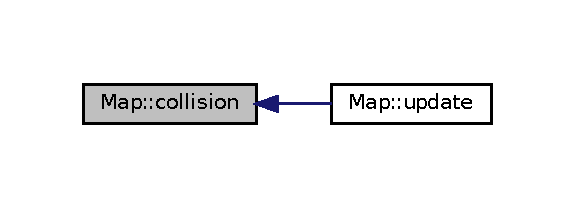
\includegraphics[width=276pt]{classMap_ae2311b25220590e05479d66408eeaabf_icgraph}
\end{center}
\end{figure}
\mbox{\Hypertarget{classMap_a8485dce46ceae190bc9f51e22885eca3}\label{classMap_a8485dce46ceae190bc9f51e22885eca3}} 
\index{Map@{Map}!C\+Pburgers@{C\+Pburgers}}
\index{C\+Pburgers@{C\+Pburgers}!Map@{Map}}
\subsubsection{\texorpdfstring{C\+Pburgers()}{CPburgers()}}
{\footnotesize\ttfamily void Map\+::\+C\+Pburgers (\begin{DoxyParamCaption}{ }\end{DoxyParamCaption})}



Spawn all the burgers based on the tile map. 


\begin{DoxyParams}{Parameters}
{\em delta\+Time} & Pace timing. \\
\hline
\end{DoxyParams}
Here is the caller graph for this function\+:\nopagebreak
\begin{figure}[H]
\begin{center}
\leavevmode
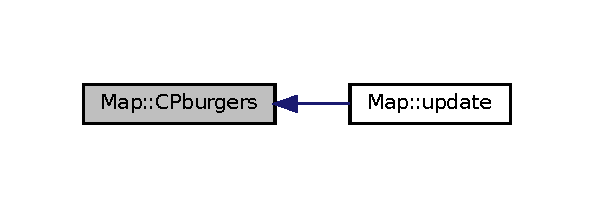
\includegraphics[width=285pt]{classMap_a8485dce46ceae190bc9f51e22885eca3_icgraph}
\end{center}
\end{figure}
\mbox{\Hypertarget{classMap_a3d0c3cf82f949ab01c788ab1c3e7f799}\label{classMap_a3d0c3cf82f949ab01c788ab1c3e7f799}} 
\index{Map@{Map}!Draw\+Map@{Draw\+Map}}
\index{Draw\+Map@{Draw\+Map}!Map@{Map}}
\subsubsection{\texorpdfstring{Draw\+Map()}{DrawMap()}}
{\footnotesize\ttfamily void Map\+::\+Draw\+Map (\begin{DoxyParamCaption}\item[{float}]{delta\+Time }\end{DoxyParamCaption})}



Updates the menu frames. 


\begin{DoxyParams}{Parameters}
{\em delta\+Time} & Pace timing. \\
\hline
\end{DoxyParams}
\mbox{\Hypertarget{classMap_af58f98cfacd972d950201cc25df95982}\label{classMap_af58f98cfacd972d950201cc25df95982}} 
\index{Map@{Map}!End\+Game@{End\+Game}}
\index{End\+Game@{End\+Game}!Map@{Map}}
\subsubsection{\texorpdfstring{End\+Game()}{EndGame()}}
{\footnotesize\ttfamily void Map\+::\+End\+Game (\begin{DoxyParamCaption}{ }\end{DoxyParamCaption})}



Checks if the game has ended. 

Here is the caller graph for this function\+:\nopagebreak
\begin{figure}[H]
\begin{center}
\leavevmode
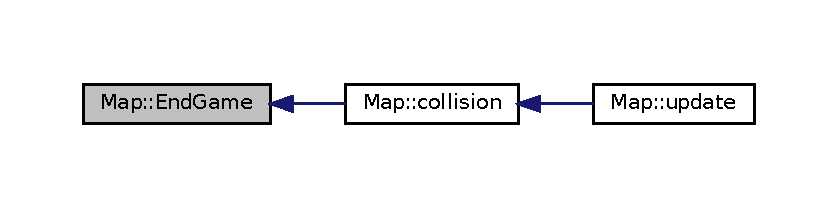
\includegraphics[width=350pt]{classMap_af58f98cfacd972d950201cc25df95982_icgraph}
\end{center}
\end{figure}
\mbox{\Hypertarget{classMap_a0c46c2c55236317c42854758b1af682f}\label{classMap_a0c46c2c55236317c42854758b1af682f}} 
\index{Map@{Map}!Get\+Size@{Get\+Size}}
\index{Get\+Size@{Get\+Size}!Map@{Map}}
\subsubsection{\texorpdfstring{Get\+Size()}{GetSize()}}
{\footnotesize\ttfamily sf\+::\+Vector2f Map\+::\+Get\+Size (\begin{DoxyParamCaption}{ }\end{DoxyParamCaption}) const}



Get map size. 

\mbox{\Hypertarget{classMap_a67b222c575eee96246c2f3fd25b4912c}\label{classMap_a67b222c575eee96246c2f3fd25b4912c}} 
\index{Map@{Map}!Init@{Init}}
\index{Init@{Init}!Map@{Map}}
\subsubsection{\texorpdfstring{Init()}{Init()}}
{\footnotesize\ttfamily void Map\+::\+Init (\begin{DoxyParamCaption}{ }\end{DoxyParamCaption})}



Initializes all the needed parts of the map. 

\mbox{\Hypertarget{classMap_a63ecd67d43e63befe38de3e438abedff}\label{classMap_a63ecd67d43e63befe38de3e438abedff}} 
\index{Map@{Map}!load\+Textures@{load\+Textures}}
\index{load\+Textures@{load\+Textures}!Map@{Map}}
\subsubsection{\texorpdfstring{load\+Textures()}{loadTextures()}}
{\footnotesize\ttfamily void Map\+::load\+Textures (\begin{DoxyParamCaption}\item[{std\+::string}]{file\+Name }\end{DoxyParamCaption})}



Updates the menu frames. 


\begin{DoxyParams}{Parameters}
{\em delta\+Time} & Pace timing. \\
\hline
\end{DoxyParams}
Here is the call graph for this function\+:\nopagebreak
\begin{figure}[H]
\begin{center}
\leavevmode
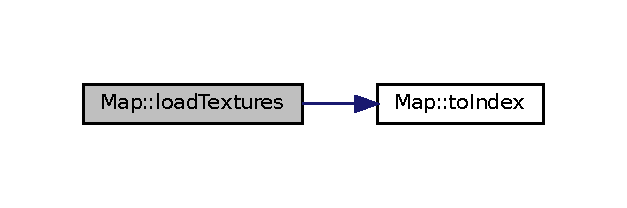
\includegraphics[width=301pt]{classMap_a63ecd67d43e63befe38de3e438abedff_cgraph}
\end{center}
\end{figure}
\mbox{\Hypertarget{classMap_a378ff701ba69cfe800693466f8f3299e}\label{classMap_a378ff701ba69cfe800693466f8f3299e}} 
\index{Map@{Map}!to\+Index@{to\+Index}}
\index{to\+Index@{to\+Index}!Map@{Map}}
\subsubsection{\texorpdfstring{to\+Index()}{toIndex()}\hspace{0.1cm}{\footnotesize\ttfamily [1/2]}}
{\footnotesize\ttfamily int Map\+::to\+Index (\begin{DoxyParamCaption}\item[{int}]{x,  }\item[{int}]{y }\end{DoxyParamCaption})}



Transforms x and y intro the right the index of the tile map vector. 


\begin{DoxyParams}{Parameters}
{\em x} & X-\/axis coordinate. \\
\hline
{\em y} & Y-\/axis coordinate \\
\hline
\end{DoxyParams}
Here is the caller graph for this function\+:\nopagebreak
\begin{figure}[H]
\begin{center}
\leavevmode
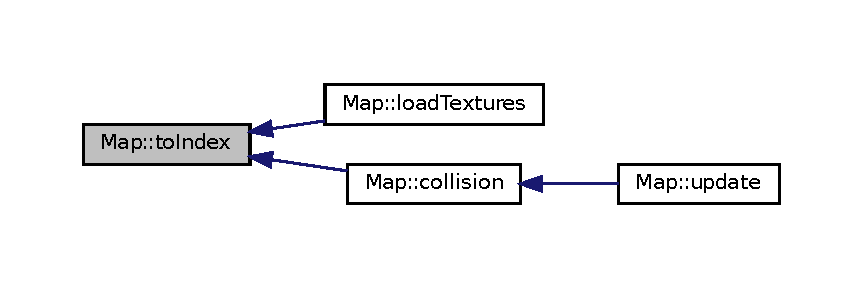
\includegraphics[width=350pt]{classMap_a378ff701ba69cfe800693466f8f3299e_icgraph}
\end{center}
\end{figure}
\mbox{\Hypertarget{classMap_a52f3ef46020dd2f6544fa2ee8dc9f4ff}\label{classMap_a52f3ef46020dd2f6544fa2ee8dc9f4ff}} 
\index{Map@{Map}!to\+Index@{to\+Index}}
\index{to\+Index@{to\+Index}!Map@{Map}}
\subsubsection{\texorpdfstring{to\+Index()}{toIndex()}\hspace{0.1cm}{\footnotesize\ttfamily [2/2]}}
{\footnotesize\ttfamily int Map\+::to\+Index (\begin{DoxyParamCaption}\item[{sf\+::\+Vector2i}]{vec }\end{DoxyParamCaption})}



Transforms a vector coordinate into the vector index och the tile map. 


\begin{DoxyParams}{Parameters}
{\em vec} & Coordinate vector. \\
\hline
\end{DoxyParams}
\mbox{\Hypertarget{classMap_a7346023f96a36368daa2d4cafd4523f2}\label{classMap_a7346023f96a36368daa2d4cafd4523f2}} 
\index{Map@{Map}!update@{update}}
\index{update@{update}!Map@{Map}}
\subsubsection{\texorpdfstring{update()}{update()}}
{\footnotesize\ttfamily void Map\+::update (\begin{DoxyParamCaption}\item[{float}]{delta\+Time,  }\item[{sf\+::\+Render\+Window \&}]{window }\end{DoxyParamCaption})}



Updates the menu frames. 


\begin{DoxyParams}{Parameters}
{\em delta\+Time} & Pace timing. \\
\hline
{\em window} & Reference to the game window. \\
\hline
\end{DoxyParams}
Here is the call graph for this function\+:\nopagebreak
\begin{figure}[H]
\begin{center}
\leavevmode
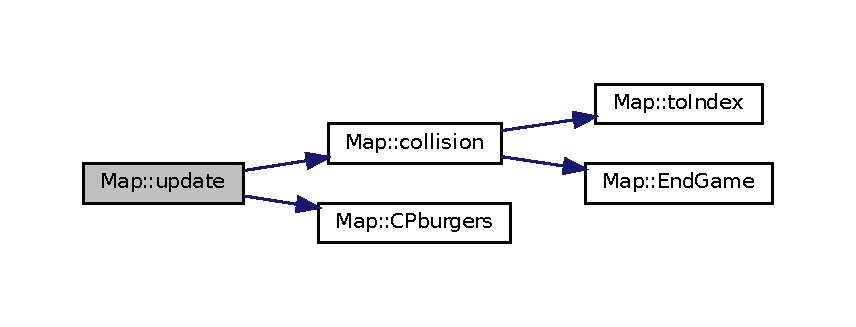
\includegraphics[width=350pt]{classMap_a7346023f96a36368daa2d4cafd4523f2_cgraph}
\end{center}
\end{figure}


\subsection{Friends And Related Function Documentation}
\mbox{\Hypertarget{classMap_a8a97b6d5e408db103798551949a4e1f8}\label{classMap_a8a97b6d5e408db103798551949a4e1f8}} 
\index{Map@{Map}!Stage\+One@{Stage\+One}}
\index{Stage\+One@{Stage\+One}!Map@{Map}}
\subsubsection{\texorpdfstring{Stage\+One}{StageOne}}
{\footnotesize\ttfamily friend class \mbox{\hyperlink{classStageOne}{Stage\+One}}\hspace{0.3cm}{\ttfamily [friend]}}



The documentation for this class was generated from the following files\+:\begin{DoxyCompactItemize}
\item 
\mbox{\hyperlink{Map_8h}{Map.\+h}}\item 
\mbox{\hyperlink{Map_8cpp}{Map.\+cpp}}\end{DoxyCompactItemize}

\hypertarget{classMenu}{}\section{Menu Class Reference}
\label{classMenu}\index{Menu@{Menu}}


{\ttfamily \#include $<$Menu.\+h$>$}



Inheritance diagram for Menu\+:\nopagebreak
\begin{figure}[H]
\begin{center}
\leavevmode
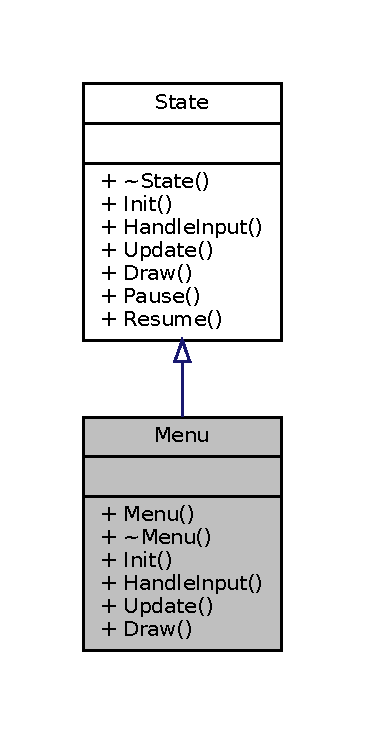
\includegraphics[width=175pt]{classMenu__inherit__graph}
\end{center}
\end{figure}


Collaboration diagram for Menu\+:\nopagebreak
\begin{figure}[H]
\begin{center}
\leavevmode
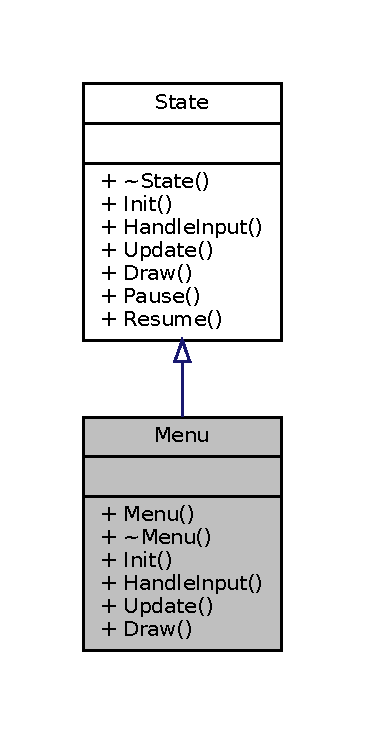
\includegraphics[width=175pt]{classMenu__coll__graph}
\end{center}
\end{figure}
\subsection*{Public Member Functions}
\begin{DoxyCompactItemize}
\item 
\mbox{\hyperlink{classMenu_a15b3521b67715170d4aaa6324003cc11}{Menu}} (\mbox{\hyperlink{Game_8h_aff850703a7797c8bfee2f02906aec50c}{Game\+Data\+Ref}} data)
\item 
\mbox{\hyperlink{classMenu_a831387f51358cfb88cd018e1777bc980}{$\sim$\+Menu}} ()
\item 
void \mbox{\hyperlink{classMenu_a2d4c37774fe4c5efe08ee436b0bb1c76}{Init}} ()
\item 
void \mbox{\hyperlink{classMenu_a0cb3596524ed7fd021f999860b563bf8}{Handle\+Input}} ()
\begin{DoxyCompactList}\small\item\em Handles mouse input from the player. \end{DoxyCompactList}\item 
void \mbox{\hyperlink{classMenu_a4d5311d60fb41b4d0498a6fc820088be}{Update}} (float delta\+Time)
\begin{DoxyCompactList}\small\item\em Updates the menu frames. \end{DoxyCompactList}\item 
void \mbox{\hyperlink{classMenu_a510885af1fe41d02c1669fca278f7eed}{Draw}} (float delta\+Time)
\begin{DoxyCompactList}\small\item\em Updates the menu frames. \end{DoxyCompactList}\end{DoxyCompactItemize}


\subsection{Detailed Description}
\mbox{\hyperlink{classMenu}{Menu}} class, first stage where the player decides to play. 

\subsection{Constructor \& Destructor Documentation}
\mbox{\Hypertarget{classMenu_a15b3521b67715170d4aaa6324003cc11}\label{classMenu_a15b3521b67715170d4aaa6324003cc11}} 
\index{Menu@{Menu}!Menu@{Menu}}
\index{Menu@{Menu}!Menu@{Menu}}
\subsubsection{\texorpdfstring{Menu()}{Menu()}}
{\footnotesize\ttfamily Menu\+::\+Menu (\begin{DoxyParamCaption}\item[{\mbox{\hyperlink{Game_8h_aff850703a7797c8bfee2f02906aec50c}{Game\+Data\+Ref}}}]{data }\end{DoxyParamCaption})}

\mbox{\Hypertarget{classMenu_a831387f51358cfb88cd018e1777bc980}\label{classMenu_a831387f51358cfb88cd018e1777bc980}} 
\index{Menu@{Menu}!````~Menu@{$\sim$\+Menu}}
\index{````~Menu@{$\sim$\+Menu}!Menu@{Menu}}
\subsubsection{\texorpdfstring{$\sim$\+Menu()}{~Menu()}}
{\footnotesize\ttfamily Menu\+::$\sim$\+Menu (\begin{DoxyParamCaption}{ }\end{DoxyParamCaption})}



\subsection{Member Function Documentation}
\mbox{\Hypertarget{classMenu_a510885af1fe41d02c1669fca278f7eed}\label{classMenu_a510885af1fe41d02c1669fca278f7eed}} 
\index{Menu@{Menu}!Draw@{Draw}}
\index{Draw@{Draw}!Menu@{Menu}}
\subsubsection{\texorpdfstring{Draw()}{Draw()}}
{\footnotesize\ttfamily void Menu\+::\+Draw (\begin{DoxyParamCaption}\item[{float}]{delta\+Time }\end{DoxyParamCaption})\hspace{0.3cm}{\ttfamily [virtual]}}



Updates the menu frames. 


\begin{DoxyParams}{Parameters}
{\em delta\+Time} & Pace timing. \\
\hline
\end{DoxyParams}


Implements \mbox{\hyperlink{classState_ae3bc988c6103665bca68560742fb40e1}{State}}.

\mbox{\Hypertarget{classMenu_a0cb3596524ed7fd021f999860b563bf8}\label{classMenu_a0cb3596524ed7fd021f999860b563bf8}} 
\index{Menu@{Menu}!Handle\+Input@{Handle\+Input}}
\index{Handle\+Input@{Handle\+Input}!Menu@{Menu}}
\subsubsection{\texorpdfstring{Handle\+Input()}{HandleInput()}}
{\footnotesize\ttfamily void Menu\+::\+Handle\+Input (\begin{DoxyParamCaption}{ }\end{DoxyParamCaption})\hspace{0.3cm}{\ttfamily [virtual]}}



Handles mouse input from the player. 



Implements \mbox{\hyperlink{classState_ad3de659bdeb45c97486464461d625e8f}{State}}.

Here is the call graph for this function\+:\nopagebreak
\begin{figure}[H]
\begin{center}
\leavevmode
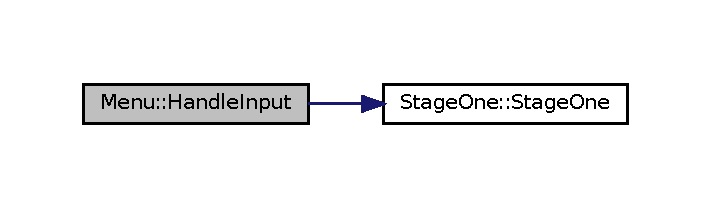
\includegraphics[width=341pt]{classMenu_a0cb3596524ed7fd021f999860b563bf8_cgraph}
\end{center}
\end{figure}
\mbox{\Hypertarget{classMenu_a2d4c37774fe4c5efe08ee436b0bb1c76}\label{classMenu_a2d4c37774fe4c5efe08ee436b0bb1c76}} 
\index{Menu@{Menu}!Init@{Init}}
\index{Init@{Init}!Menu@{Menu}}
\subsubsection{\texorpdfstring{Init()}{Init()}}
{\footnotesize\ttfamily void Menu\+::\+Init (\begin{DoxyParamCaption}{ }\end{DoxyParamCaption})\hspace{0.3cm}{\ttfamily [virtual]}}



Implements \mbox{\hyperlink{classState_a7ab4d8c6aa239a17ed579d89a209b156}{State}}.

\mbox{\Hypertarget{classMenu_a4d5311d60fb41b4d0498a6fc820088be}\label{classMenu_a4d5311d60fb41b4d0498a6fc820088be}} 
\index{Menu@{Menu}!Update@{Update}}
\index{Update@{Update}!Menu@{Menu}}
\subsubsection{\texorpdfstring{Update()}{Update()}}
{\footnotesize\ttfamily void Menu\+::\+Update (\begin{DoxyParamCaption}\item[{float}]{delta\+Time }\end{DoxyParamCaption})\hspace{0.3cm}{\ttfamily [virtual]}}



Updates the menu frames. 


\begin{DoxyParams}{Parameters}
{\em delta\+Time} & Pace timing. \\
\hline
\end{DoxyParams}


Implements \mbox{\hyperlink{classState_a770f40188fdfc64bc95a5166fef12e02}{State}}.



The documentation for this class was generated from the following files\+:\begin{DoxyCompactItemize}
\item 
\mbox{\hyperlink{Menu_8h}{Menu.\+h}}\item 
\mbox{\hyperlink{Menu_8cpp}{Menu.\+cpp}}\end{DoxyCompactItemize}

\hypertarget{classPlayer}{}\section{Player Class Reference}
\label{classPlayer}\index{Player@{Player}}


{\ttfamily \#include $<$Player.\+h$>$}



Collaboration diagram for Player\+:\nopagebreak
\begin{figure}[H]
\begin{center}
\leavevmode
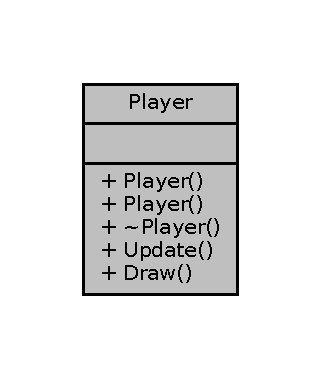
\includegraphics[width=154pt]{classPlayer__coll__graph}
\end{center}
\end{figure}
\subsection*{Public Member Functions}
\begin{DoxyCompactItemize}
\item 
\mbox{\hyperlink{classPlayer_a314e533783ad3c376a43cad3f49efa0c}{Player}} ()=delete
\item 
\mbox{\hyperlink{classPlayer_a033e19f2fd9948f3aad73cd82a404f8e}{Player}} (sf\+::\+Texture \&texture, sf\+::\+Vector2u image\+Count, float switch\+Time)
\begin{DoxyCompactList}\small\item\em Creaters the player. \end{DoxyCompactList}\item 
\mbox{\hyperlink{classPlayer_a749d2c00e1fe0f5c2746f7505a58c062}{$\sim$\+Player}} ()
\item 
void \mbox{\hyperlink{classPlayer_ae6b2acaf61aae4df8e10f50ebbdf664d}{Update}} (float delta\+Time)
\begin{DoxyCompactList}\small\item\em Updates the player position. \end{DoxyCompactList}\item 
void \mbox{\hyperlink{classPlayer_a6a0b48c845f9c341283b5fc5a7898f9b}{Draw}} (sf\+::\+Render\+Window \&window)
\begin{DoxyCompactList}\small\item\em Updates the player position. \end{DoxyCompactList}\end{DoxyCompactItemize}
\subsection*{Friends}
\begin{DoxyCompactItemize}
\item 
class \mbox{\hyperlink{classPlayer_ad2f32e921244459f7cc6d50355429cc6}{Map}}
\end{DoxyCompactItemize}


\subsection{Detailed Description}
\mbox{\hyperlink{classPlayer}{Player}} class, herer will all the character attibutes be decided. 

\subsection{Constructor \& Destructor Documentation}
\mbox{\Hypertarget{classPlayer_a314e533783ad3c376a43cad3f49efa0c}\label{classPlayer_a314e533783ad3c376a43cad3f49efa0c}} 
\index{Player@{Player}!Player@{Player}}
\index{Player@{Player}!Player@{Player}}
\subsubsection{\texorpdfstring{Player()}{Player()}\hspace{0.1cm}{\footnotesize\ttfamily [1/2]}}
{\footnotesize\ttfamily Player\+::\+Player (\begin{DoxyParamCaption}{ }\end{DoxyParamCaption})\hspace{0.3cm}{\ttfamily [delete]}}

\mbox{\Hypertarget{classPlayer_a033e19f2fd9948f3aad73cd82a404f8e}\label{classPlayer_a033e19f2fd9948f3aad73cd82a404f8e}} 
\index{Player@{Player}!Player@{Player}}
\index{Player@{Player}!Player@{Player}}
\subsubsection{\texorpdfstring{Player()}{Player()}\hspace{0.1cm}{\footnotesize\ttfamily [2/2]}}
{\footnotesize\ttfamily Player\+::\+Player (\begin{DoxyParamCaption}\item[{sf\+::\+Texture \&}]{texture,  }\item[{sf\+::\+Vector2u}]{image\+Count,  }\item[{float}]{switch\+Time }\end{DoxyParamCaption})}



Creaters the player. 


\begin{DoxyParams}{Parameters}
{\em texture} & Is the player texture. \\
\hline
{\em image\+Count} & Number of images in the character animation grid. \\
\hline
{\em switch\+Time} & How fast should the animation loob be. \\
\hline
\end{DoxyParams}
\mbox{\Hypertarget{classPlayer_a749d2c00e1fe0f5c2746f7505a58c062}\label{classPlayer_a749d2c00e1fe0f5c2746f7505a58c062}} 
\index{Player@{Player}!````~Player@{$\sim$\+Player}}
\index{````~Player@{$\sim$\+Player}!Player@{Player}}
\subsubsection{\texorpdfstring{$\sim$\+Player()}{~Player()}}
{\footnotesize\ttfamily Player\+::$\sim$\+Player (\begin{DoxyParamCaption}{ }\end{DoxyParamCaption})}



\subsection{Member Function Documentation}
\mbox{\Hypertarget{classPlayer_a6a0b48c845f9c341283b5fc5a7898f9b}\label{classPlayer_a6a0b48c845f9c341283b5fc5a7898f9b}} 
\index{Player@{Player}!Draw@{Draw}}
\index{Draw@{Draw}!Player@{Player}}
\subsubsection{\texorpdfstring{Draw()}{Draw()}}
{\footnotesize\ttfamily void Player\+::\+Draw (\begin{DoxyParamCaption}\item[{sf\+::\+Render\+Window \&}]{window }\end{DoxyParamCaption})}



Updates the player position. 


\begin{DoxyParams}{Parameters}
{\em window} & \mbox{\hyperlink{classGame}{Game}} window. \\
\hline
\end{DoxyParams}
\mbox{\Hypertarget{classPlayer_ae6b2acaf61aae4df8e10f50ebbdf664d}\label{classPlayer_ae6b2acaf61aae4df8e10f50ebbdf664d}} 
\index{Player@{Player}!Update@{Update}}
\index{Update@{Update}!Player@{Player}}
\subsubsection{\texorpdfstring{Update()}{Update()}}
{\footnotesize\ttfamily void Player\+::\+Update (\begin{DoxyParamCaption}\item[{float}]{delta\+Time }\end{DoxyParamCaption})}



Updates the player position. 


\begin{DoxyParams}{Parameters}
{\em delta\+Time} & Pace the character is moving. \\
\hline
\end{DoxyParams}
Here is the call graph for this function\+:
\nopagebreak
\begin{figure}[H]
\begin{center}
\leavevmode
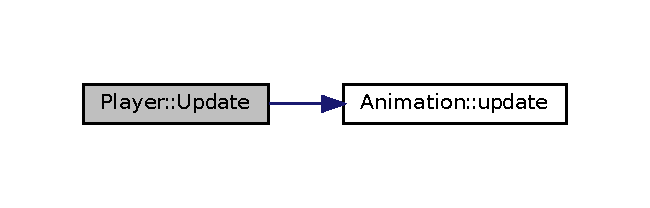
\includegraphics[width=312pt]{classPlayer_ae6b2acaf61aae4df8e10f50ebbdf664d_cgraph}
\end{center}
\end{figure}


\subsection{Friends And Related Function Documentation}
\mbox{\Hypertarget{classPlayer_ad2f32e921244459f7cc6d50355429cc6}\label{classPlayer_ad2f32e921244459f7cc6d50355429cc6}} 
\index{Player@{Player}!Map@{Map}}
\index{Map@{Map}!Player@{Player}}
\subsubsection{\texorpdfstring{Map}{Map}}
{\footnotesize\ttfamily friend class \mbox{\hyperlink{classMap}{Map}}\hspace{0.3cm}{\ttfamily [friend]}}



The documentation for this class was generated from the following files\+:\begin{DoxyCompactItemize}
\item 
\mbox{\hyperlink{Player_8h}{Player.\+h}}\item 
\mbox{\hyperlink{Player_8cpp}{Player.\+cpp}}\end{DoxyCompactItemize}

\hypertarget{classStageOne}{}\section{Stage\+One Class Reference}
\label{classStageOne}\index{Stage\+One@{Stage\+One}}


{\ttfamily \#include $<$Stage\+One.\+h$>$}



Inheritance diagram for Stage\+One\+:\nopagebreak
\begin{figure}[H]
\begin{center}
\leavevmode
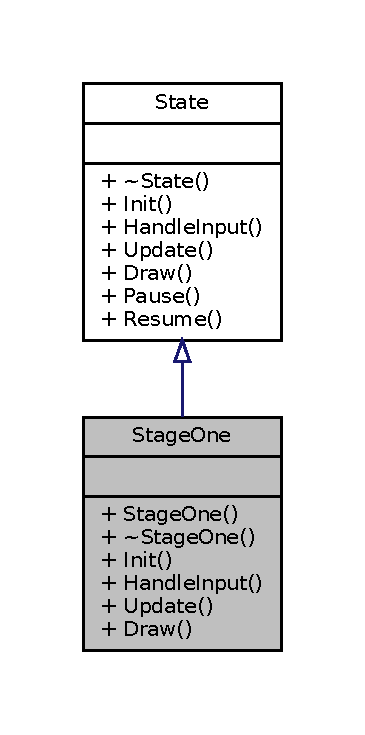
\includegraphics[width=175pt]{classStageOne__inherit__graph}
\end{center}
\end{figure}


Collaboration diagram for Stage\+One\+:\nopagebreak
\begin{figure}[H]
\begin{center}
\leavevmode
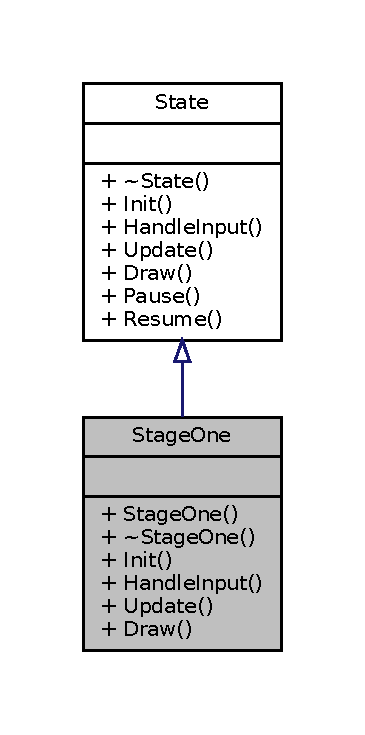
\includegraphics[width=175pt]{classStageOne__coll__graph}
\end{center}
\end{figure}
\subsection*{Public Member Functions}
\begin{DoxyCompactItemize}
\item 
\mbox{\hyperlink{classStageOne_a9eb31d0ce98795803b764b8836493008}{Stage\+One}} (\mbox{\hyperlink{Game_8h_aff850703a7797c8bfee2f02906aec50c}{Game\+Data\+Ref}} data)
\item 
\mbox{\hyperlink{classStageOne_a7761fca03288159de1772c59b31839d2}{$\sim$\+Stage\+One}} ()
\item 
void \mbox{\hyperlink{classStageOne_a661f4913ad0f6cc348c19bfa86c0c489}{Init}} ()
\item 
void \mbox{\hyperlink{classStageOne_a168fa7a88a44900ab5d91bfe87150221}{Handle\+Input}} ()
\item 
void \mbox{\hyperlink{classStageOne_aa26da852d0927aace63f7054fa097e2a}{Update}} (float delta\+Time)
\begin{DoxyCompactList}\small\item\em Updates the \mbox{\hyperlink{classStageOne}{Stage\+One}}. \end{DoxyCompactList}\item 
void \mbox{\hyperlink{classStageOne_af59dff5e563f4d1f45ea4b8708a3301e}{Draw}} (float delta\+Time)
\begin{DoxyCompactList}\small\item\em Updates the \mbox{\hyperlink{classStageOne}{Stage\+One}}. \end{DoxyCompactList}\end{DoxyCompactItemize}


\subsection{Detailed Description}
Stage One \mbox{\hyperlink{classState}{State}}. Creatures, map, player gets initialized and starts the first game stage. 

\subsection{Constructor \& Destructor Documentation}
\mbox{\Hypertarget{classStageOne_a9eb31d0ce98795803b764b8836493008}\label{classStageOne_a9eb31d0ce98795803b764b8836493008}} 
\index{Stage\+One@{Stage\+One}!Stage\+One@{Stage\+One}}
\index{Stage\+One@{Stage\+One}!Stage\+One@{Stage\+One}}
\subsubsection{\texorpdfstring{Stage\+One()}{StageOne()}}
{\footnotesize\ttfamily Stage\+One\+::\+Stage\+One (\begin{DoxyParamCaption}\item[{\mbox{\hyperlink{Game_8h_aff850703a7797c8bfee2f02906aec50c}{Game\+Data\+Ref}}}]{data }\end{DoxyParamCaption})}

Here is the caller graph for this function\+:\nopagebreak
\begin{figure}[H]
\begin{center}
\leavevmode
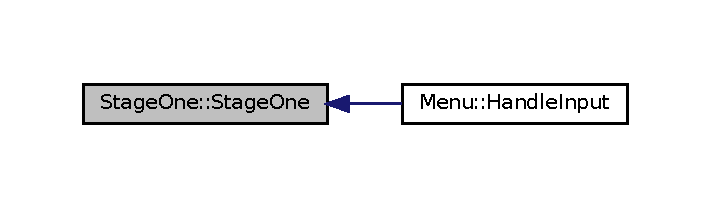
\includegraphics[width=341pt]{classStageOne_a9eb31d0ce98795803b764b8836493008_icgraph}
\end{center}
\end{figure}
\mbox{\Hypertarget{classStageOne_a7761fca03288159de1772c59b31839d2}\label{classStageOne_a7761fca03288159de1772c59b31839d2}} 
\index{Stage\+One@{Stage\+One}!````~Stage\+One@{$\sim$\+Stage\+One}}
\index{````~Stage\+One@{$\sim$\+Stage\+One}!Stage\+One@{Stage\+One}}
\subsubsection{\texorpdfstring{$\sim$\+Stage\+One()}{~StageOne()}}
{\footnotesize\ttfamily Stage\+One\+::$\sim$\+Stage\+One (\begin{DoxyParamCaption}{ }\end{DoxyParamCaption})}



\subsection{Member Function Documentation}
\mbox{\Hypertarget{classStageOne_af59dff5e563f4d1f45ea4b8708a3301e}\label{classStageOne_af59dff5e563f4d1f45ea4b8708a3301e}} 
\index{Stage\+One@{Stage\+One}!Draw@{Draw}}
\index{Draw@{Draw}!Stage\+One@{Stage\+One}}
\subsubsection{\texorpdfstring{Draw()}{Draw()}}
{\footnotesize\ttfamily void Stage\+One\+::\+Draw (\begin{DoxyParamCaption}\item[{float}]{delta\+Time }\end{DoxyParamCaption})\hspace{0.3cm}{\ttfamily [virtual]}}



Updates the \mbox{\hyperlink{classStageOne}{Stage\+One}}. 


\begin{DoxyParams}{Parameters}
{\em delta\+Time} & needs the delta\+Time so the objects run at the same pace in different machines. \\
\hline
\end{DoxyParams}


Implements \mbox{\hyperlink{classState_ae3bc988c6103665bca68560742fb40e1}{State}}.

\mbox{\Hypertarget{classStageOne_a168fa7a88a44900ab5d91bfe87150221}\label{classStageOne_a168fa7a88a44900ab5d91bfe87150221}} 
\index{Stage\+One@{Stage\+One}!Handle\+Input@{Handle\+Input}}
\index{Handle\+Input@{Handle\+Input}!Stage\+One@{Stage\+One}}
\subsubsection{\texorpdfstring{Handle\+Input()}{HandleInput()}}
{\footnotesize\ttfamily void Stage\+One\+::\+Handle\+Input (\begin{DoxyParamCaption}{ }\end{DoxyParamCaption})\hspace{0.3cm}{\ttfamily [virtual]}}



Implements \mbox{\hyperlink{classState_ad3de659bdeb45c97486464461d625e8f}{State}}.

\mbox{\Hypertarget{classStageOne_a661f4913ad0f6cc348c19bfa86c0c489}\label{classStageOne_a661f4913ad0f6cc348c19bfa86c0c489}} 
\index{Stage\+One@{Stage\+One}!Init@{Init}}
\index{Init@{Init}!Stage\+One@{Stage\+One}}
\subsubsection{\texorpdfstring{Init()}{Init()}}
{\footnotesize\ttfamily void Stage\+One\+::\+Init (\begin{DoxyParamCaption}{ }\end{DoxyParamCaption})\hspace{0.3cm}{\ttfamily [virtual]}}



Implements \mbox{\hyperlink{classState_a7ab4d8c6aa239a17ed579d89a209b156}{State}}.

\mbox{\Hypertarget{classStageOne_aa26da852d0927aace63f7054fa097e2a}\label{classStageOne_aa26da852d0927aace63f7054fa097e2a}} 
\index{Stage\+One@{Stage\+One}!Update@{Update}}
\index{Update@{Update}!Stage\+One@{Stage\+One}}
\subsubsection{\texorpdfstring{Update()}{Update()}}
{\footnotesize\ttfamily void Stage\+One\+::\+Update (\begin{DoxyParamCaption}\item[{float}]{delta\+Time }\end{DoxyParamCaption})\hspace{0.3cm}{\ttfamily [virtual]}}



Updates the \mbox{\hyperlink{classStageOne}{Stage\+One}}. 


\begin{DoxyParams}{Parameters}
{\em delta\+Time} & needs the delta\+Time so the objects run at the same pace in different machines. \\
\hline
\end{DoxyParams}


Implements \mbox{\hyperlink{classState_a770f40188fdfc64bc95a5166fef12e02}{State}}.



The documentation for this class was generated from the following files\+:\begin{DoxyCompactItemize}
\item 
\mbox{\hyperlink{StageOne_8h}{Stage\+One.\+h}}\item 
\mbox{\hyperlink{StageOne_8cpp}{Stage\+One.\+cpp}}\end{DoxyCompactItemize}

\hypertarget{classState}{}\section{State Class Reference}
\label{classState}\index{State@{State}}


{\ttfamily \#include $<$State.\+h$>$}



Inheritance diagram for State\+:\nopagebreak
\begin{figure}[H]
\begin{center}
\leavevmode
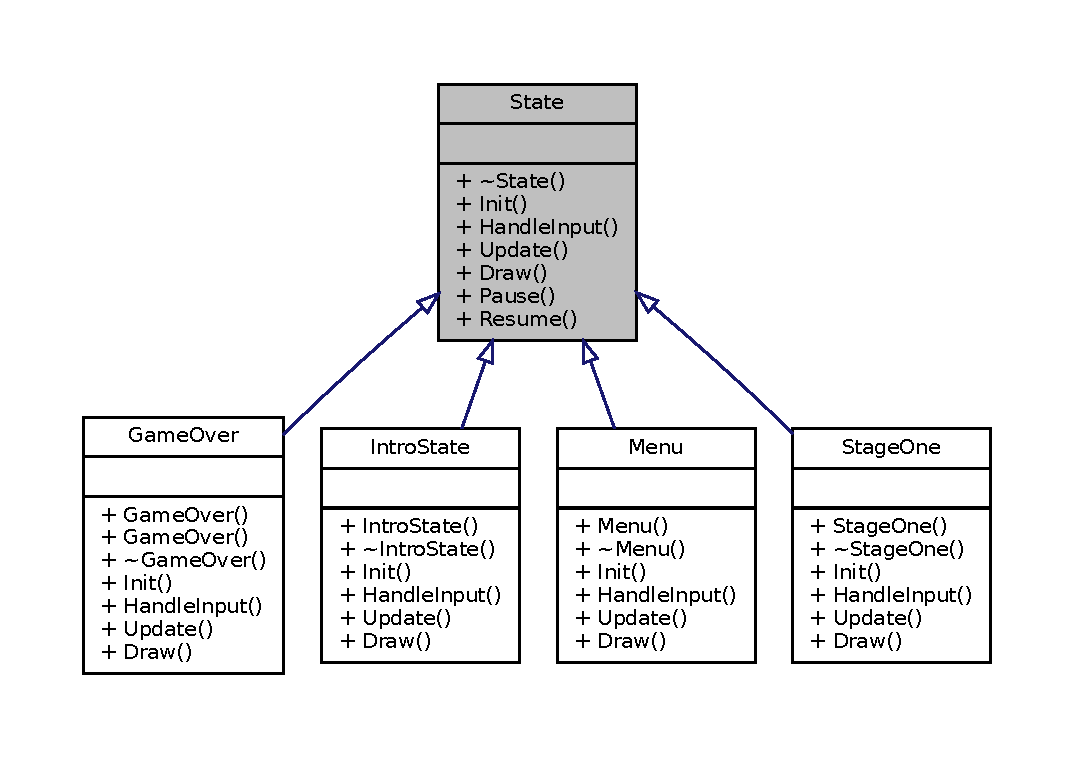
\includegraphics[width=350pt]{classState__inherit__graph}
\end{center}
\end{figure}


Collaboration diagram for State\+:\nopagebreak
\begin{figure}[H]
\begin{center}
\leavevmode
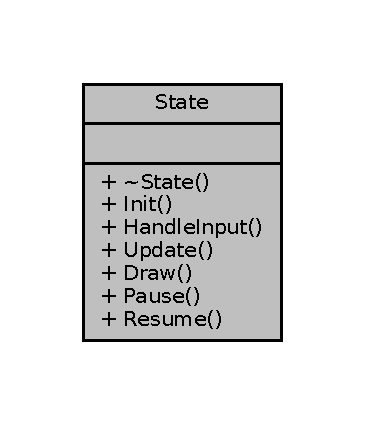
\includegraphics[width=175pt]{classState__coll__graph}
\end{center}
\end{figure}
\subsection*{Public Member Functions}
\begin{DoxyCompactItemize}
\item 
virtual \mbox{\hyperlink{classState_a9ddc1df6f998184d6477b48fab90281c}{$\sim$\+State}} ()
\item 
virtual void \mbox{\hyperlink{classState_a7ab4d8c6aa239a17ed579d89a209b156}{Init}} ()=0
\item 
virtual void \mbox{\hyperlink{classState_ad3de659bdeb45c97486464461d625e8f}{Handle\+Input}} ()=0
\item 
virtual void \mbox{\hyperlink{classState_a770f40188fdfc64bc95a5166fef12e02}{Update}} (float delta\+Time)=0
\item 
virtual void \mbox{\hyperlink{classState_ae3bc988c6103665bca68560742fb40e1}{Draw}} (float delta\+Time)=0
\item 
virtual void \mbox{\hyperlink{classState_aeba18061e63cd52551a045fb94836298}{Pause}} ()
\item 
virtual void \mbox{\hyperlink{classState_a8c585ea3e766c2e2404a957907310983}{Resume}} ()
\end{DoxyCompactItemize}


\subsection{Detailed Description}
Abstract class where the derivatives of it will be the stages of the game. 

\subsection{Constructor \& Destructor Documentation}
\mbox{\Hypertarget{classState_a9ddc1df6f998184d6477b48fab90281c}\label{classState_a9ddc1df6f998184d6477b48fab90281c}} 
\index{State@{State}!````~State@{$\sim$\+State}}
\index{````~State@{$\sim$\+State}!State@{State}}
\subsubsection{\texorpdfstring{$\sim$\+State()}{~State()}}
{\footnotesize\ttfamily virtual State\+::$\sim$\+State (\begin{DoxyParamCaption}{ }\end{DoxyParamCaption})\hspace{0.3cm}{\ttfamily [inline]}, {\ttfamily [virtual]}}



\subsection{Member Function Documentation}
\mbox{\Hypertarget{classState_ae3bc988c6103665bca68560742fb40e1}\label{classState_ae3bc988c6103665bca68560742fb40e1}} 
\index{State@{State}!Draw@{Draw}}
\index{Draw@{Draw}!State@{State}}
\subsubsection{\texorpdfstring{Draw()}{Draw()}}
{\footnotesize\ttfamily virtual void State\+::\+Draw (\begin{DoxyParamCaption}\item[{float}]{delta\+Time }\end{DoxyParamCaption})\hspace{0.3cm}{\ttfamily [pure virtual]}}



Implemented in \mbox{\hyperlink{classStageOne_af59dff5e563f4d1f45ea4b8708a3301e}{Stage\+One}}, \mbox{\hyperlink{classIntroState_a903b8e2b781eae1e9a6e7db08d38fd2c}{Intro\+State}}, \mbox{\hyperlink{classMenu_a510885af1fe41d02c1669fca278f7eed}{Menu}}, and \mbox{\hyperlink{classGameOver_a263a49026ce81b22721cfc515f8efd4e}{Game\+Over}}.

\mbox{\Hypertarget{classState_ad3de659bdeb45c97486464461d625e8f}\label{classState_ad3de659bdeb45c97486464461d625e8f}} 
\index{State@{State}!Handle\+Input@{Handle\+Input}}
\index{Handle\+Input@{Handle\+Input}!State@{State}}
\subsubsection{\texorpdfstring{Handle\+Input()}{HandleInput()}}
{\footnotesize\ttfamily virtual void State\+::\+Handle\+Input (\begin{DoxyParamCaption}{ }\end{DoxyParamCaption})\hspace{0.3cm}{\ttfamily [pure virtual]}}



Implemented in \mbox{\hyperlink{classStageOne_a168fa7a88a44900ab5d91bfe87150221}{Stage\+One}}, \mbox{\hyperlink{classIntroState_a6a2a89b3374f53e1bcf366c0ae896109}{Intro\+State}}, \mbox{\hyperlink{classMenu_a0cb3596524ed7fd021f999860b563bf8}{Menu}}, and \mbox{\hyperlink{classGameOver_a1b90d0ed04386fe166cbfcf2427a5175}{Game\+Over}}.

\mbox{\Hypertarget{classState_a7ab4d8c6aa239a17ed579d89a209b156}\label{classState_a7ab4d8c6aa239a17ed579d89a209b156}} 
\index{State@{State}!Init@{Init}}
\index{Init@{Init}!State@{State}}
\subsubsection{\texorpdfstring{Init()}{Init()}}
{\footnotesize\ttfamily virtual void State\+::\+Init (\begin{DoxyParamCaption}{ }\end{DoxyParamCaption})\hspace{0.3cm}{\ttfamily [pure virtual]}}



Implemented in \mbox{\hyperlink{classStageOne_a661f4913ad0f6cc348c19bfa86c0c489}{Stage\+One}}, \mbox{\hyperlink{classIntroState_a065e914b336c162b1467845c7126c920}{Intro\+State}}, \mbox{\hyperlink{classGameOver_ac13d1bd0fe9f8db0ef0301c9ec63a9e0}{Game\+Over}}, and \mbox{\hyperlink{classMenu_a2d4c37774fe4c5efe08ee436b0bb1c76}{Menu}}.

\mbox{\Hypertarget{classState_aeba18061e63cd52551a045fb94836298}\label{classState_aeba18061e63cd52551a045fb94836298}} 
\index{State@{State}!Pause@{Pause}}
\index{Pause@{Pause}!State@{State}}
\subsubsection{\texorpdfstring{Pause()}{Pause()}}
{\footnotesize\ttfamily virtual void State\+::\+Pause (\begin{DoxyParamCaption}{ }\end{DoxyParamCaption})\hspace{0.3cm}{\ttfamily [inline]}, {\ttfamily [virtual]}}

\mbox{\Hypertarget{classState_a8c585ea3e766c2e2404a957907310983}\label{classState_a8c585ea3e766c2e2404a957907310983}} 
\index{State@{State}!Resume@{Resume}}
\index{Resume@{Resume}!State@{State}}
\subsubsection{\texorpdfstring{Resume()}{Resume()}}
{\footnotesize\ttfamily virtual void State\+::\+Resume (\begin{DoxyParamCaption}{ }\end{DoxyParamCaption})\hspace{0.3cm}{\ttfamily [inline]}, {\ttfamily [virtual]}}

\mbox{\Hypertarget{classState_a770f40188fdfc64bc95a5166fef12e02}\label{classState_a770f40188fdfc64bc95a5166fef12e02}} 
\index{State@{State}!Update@{Update}}
\index{Update@{Update}!State@{State}}
\subsubsection{\texorpdfstring{Update()}{Update()}}
{\footnotesize\ttfamily virtual void State\+::\+Update (\begin{DoxyParamCaption}\item[{float}]{delta\+Time }\end{DoxyParamCaption})\hspace{0.3cm}{\ttfamily [pure virtual]}}



Implemented in \mbox{\hyperlink{classStageOne_aa26da852d0927aace63f7054fa097e2a}{Stage\+One}}, \mbox{\hyperlink{classIntroState_a781891b1db3bdbf6af228ef85c0df00a}{Intro\+State}}, \mbox{\hyperlink{classMenu_a4d5311d60fb41b4d0498a6fc820088be}{Menu}}, and \mbox{\hyperlink{classGameOver_a960c8ff2705f1fe49b49c717ee68fbc6}{Game\+Over}}.



The documentation for this class was generated from the following file\+:\begin{DoxyCompactItemize}
\item 
\mbox{\hyperlink{State_8h}{State.\+h}}\end{DoxyCompactItemize}

\hypertarget{classStateMachine}{}\section{State\+Machine Class Reference}
\label{classStateMachine}\index{State\+Machine@{State\+Machine}}


{\ttfamily \#include $<$State\+Machine.\+h$>$}



Collaboration diagram for State\+Machine\+:\nopagebreak
\begin{figure}[H]
\begin{center}
\leavevmode
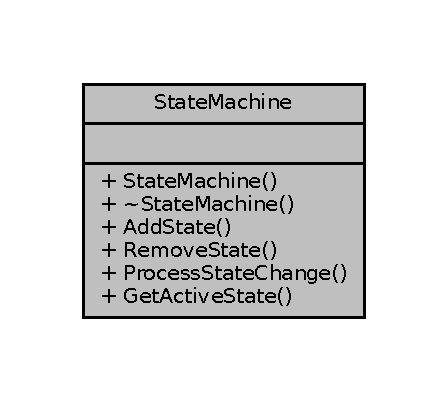
\includegraphics[width=215pt]{classStateMachine__coll__graph}
\end{center}
\end{figure}
\subsection*{Public Member Functions}
\begin{DoxyCompactItemize}
\item 
\mbox{\hyperlink{classStateMachine_a2fb07002510ea9141019559750acfab8}{State\+Machine}} ()
\item 
\mbox{\hyperlink{classStateMachine_a93d66cb2a89b186789d655a08b02674e}{$\sim$\+State\+Machine}} ()
\item 
void \mbox{\hyperlink{classStateMachine_a0ce4894da8a4f2312b1035713fb48c08}{Add\+State}} (\mbox{\hyperlink{StateMachine_8h_a217d9c9b187e9dd27abb46be48fb014d}{State\+Ref}} new\+State, bool is\+Replacing=true)
\begin{DoxyCompactList}\small\item\em Adds a game state to the stack. \end{DoxyCompactList}\item 
void \mbox{\hyperlink{classStateMachine_aebefd3cef7db9e011e15f423061d1afc}{Remove\+State}} ()
\item 
void \mbox{\hyperlink{classStateMachine_a6758b622d0428a6ed72127cd5cbf1813}{Process\+State\+Change}} ()
\item 
\mbox{\hyperlink{StateMachine_8h_a217d9c9b187e9dd27abb46be48fb014d}{State\+Ref}} \& \mbox{\hyperlink{classStateMachine_a8ae5f91aa501e0fa07478d087814906e}{Get\+Active\+State}} ()
\end{DoxyCompactItemize}


\subsection{Detailed Description}
\mbox{\hyperlink{classStateMachine}{State\+Machine}} class, this class will handle all of the differents states of the game. 

\subsection{Constructor \& Destructor Documentation}
\mbox{\Hypertarget{classStateMachine_a2fb07002510ea9141019559750acfab8}\label{classStateMachine_a2fb07002510ea9141019559750acfab8}} 
\index{State\+Machine@{State\+Machine}!State\+Machine@{State\+Machine}}
\index{State\+Machine@{State\+Machine}!State\+Machine@{State\+Machine}}
\subsubsection{\texorpdfstring{State\+Machine()}{StateMachine()}}
{\footnotesize\ttfamily State\+Machine\+::\+State\+Machine (\begin{DoxyParamCaption}{ }\end{DoxyParamCaption})}

\mbox{\Hypertarget{classStateMachine_a93d66cb2a89b186789d655a08b02674e}\label{classStateMachine_a93d66cb2a89b186789d655a08b02674e}} 
\index{State\+Machine@{State\+Machine}!````~State\+Machine@{$\sim$\+State\+Machine}}
\index{````~State\+Machine@{$\sim$\+State\+Machine}!State\+Machine@{State\+Machine}}
\subsubsection{\texorpdfstring{$\sim$\+State\+Machine()}{~StateMachine()}}
{\footnotesize\ttfamily State\+Machine\+::$\sim$\+State\+Machine (\begin{DoxyParamCaption}{ }\end{DoxyParamCaption})}



\subsection{Member Function Documentation}
\mbox{\Hypertarget{classStateMachine_a0ce4894da8a4f2312b1035713fb48c08}\label{classStateMachine_a0ce4894da8a4f2312b1035713fb48c08}} 
\index{State\+Machine@{State\+Machine}!Add\+State@{Add\+State}}
\index{Add\+State@{Add\+State}!State\+Machine@{State\+Machine}}
\subsubsection{\texorpdfstring{Add\+State()}{AddState()}}
{\footnotesize\ttfamily void State\+Machine\+::\+Add\+State (\begin{DoxyParamCaption}\item[{\mbox{\hyperlink{StateMachine_8h_a217d9c9b187e9dd27abb46be48fb014d}{State\+Ref}}}]{new\+State,  }\item[{bool}]{is\+Replacing = {\ttfamily true} }\end{DoxyParamCaption})}



Adds a game state to the stack. 


\begin{DoxyParams}{Parameters}
{\em new\+State} & Is a unique pointer to the state being added. \\
\hline
{\em is\+Replacing} & If the state is replacing there is no need of the argument, otherwise change it to false. \\
\hline
\end{DoxyParams}
\mbox{\Hypertarget{classStateMachine_a8ae5f91aa501e0fa07478d087814906e}\label{classStateMachine_a8ae5f91aa501e0fa07478d087814906e}} 
\index{State\+Machine@{State\+Machine}!Get\+Active\+State@{Get\+Active\+State}}
\index{Get\+Active\+State@{Get\+Active\+State}!State\+Machine@{State\+Machine}}
\subsubsection{\texorpdfstring{Get\+Active\+State()}{GetActiveState()}}
{\footnotesize\ttfamily \mbox{\hyperlink{StateMachine_8h_a217d9c9b187e9dd27abb46be48fb014d}{State\+Ref}} \& State\+Machine\+::\+Get\+Active\+State (\begin{DoxyParamCaption}{ }\end{DoxyParamCaption})}

Returns a referense to the active state. \mbox{\Hypertarget{classStateMachine_a6758b622d0428a6ed72127cd5cbf1813}\label{classStateMachine_a6758b622d0428a6ed72127cd5cbf1813}} 
\index{State\+Machine@{State\+Machine}!Process\+State\+Change@{Process\+State\+Change}}
\index{Process\+State\+Change@{Process\+State\+Change}!State\+Machine@{State\+Machine}}
\subsubsection{\texorpdfstring{Process\+State\+Change()}{ProcessStateChange()}}
{\footnotesize\ttfamily void State\+Machine\+::\+Process\+State\+Change (\begin{DoxyParamCaption}{ }\end{DoxyParamCaption})}

Updates the game stack. \mbox{\Hypertarget{classStateMachine_aebefd3cef7db9e011e15f423061d1afc}\label{classStateMachine_aebefd3cef7db9e011e15f423061d1afc}} 
\index{State\+Machine@{State\+Machine}!Remove\+State@{Remove\+State}}
\index{Remove\+State@{Remove\+State}!State\+Machine@{State\+Machine}}
\subsubsection{\texorpdfstring{Remove\+State()}{RemoveState()}}
{\footnotesize\ttfamily void State\+Machine\+::\+Remove\+State (\begin{DoxyParamCaption}{ }\end{DoxyParamCaption})}

Removes a state from the game stack. 

The documentation for this class was generated from the following files\+:\begin{DoxyCompactItemize}
\item 
\mbox{\hyperlink{StateMachine_8h}{State\+Machine.\+h}}\item 
\mbox{\hyperlink{StateMachine_8cpp}{State\+Machine.\+cpp}}\end{DoxyCompactItemize}

\hypertarget{structTile}{}\section{Tile Struct Reference}
\label{structTile}\index{Tile@{Tile}}


{\ttfamily \#include $<$Map.\+h$>$}



Collaboration diagram for Tile\+:\nopagebreak
\begin{figure}[H]
\begin{center}
\leavevmode
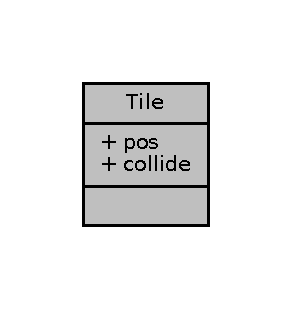
\includegraphics[width=140pt]{structTile__coll__graph}
\end{center}
\end{figure}
\subsection*{Public Attributes}
\begin{DoxyCompactItemize}
\item 
sf\+::\+Vector2i \mbox{\hyperlink{structTile_acf7dda9a45f387cff4fe0ae26ad87340}{pos}}
\item 
int \mbox{\hyperlink{structTile_a94267808f675d1644c0cb33613cc9a7e}{collide}} = 0
\end{DoxyCompactItemize}


\subsection{Detailed Description}
Struct with tile informations that are needed for collision and debuging. 

\subsection{Member Data Documentation}
\mbox{\Hypertarget{structTile_a94267808f675d1644c0cb33613cc9a7e}\label{structTile_a94267808f675d1644c0cb33613cc9a7e}} 
\index{Tile@{Tile}!collide@{collide}}
\index{collide@{collide}!Tile@{Tile}}
\subsubsection{\texorpdfstring{collide}{collide}}
{\footnotesize\ttfamily int Tile\+::collide = 0}

Does a tile have collision or not. \mbox{\Hypertarget{structTile_acf7dda9a45f387cff4fe0ae26ad87340}\label{structTile_acf7dda9a45f387cff4fe0ae26ad87340}} 
\index{Tile@{Tile}!pos@{pos}}
\index{pos@{pos}!Tile@{Tile}}
\subsubsection{\texorpdfstring{pos}{pos}}
{\footnotesize\ttfamily sf\+::\+Vector2i Tile\+::pos}

Vector with x and y position. 

The documentation for this struct was generated from the following file\+:\begin{DoxyCompactItemize}
\item 
\mbox{\hyperlink{Map_8h}{Map.\+h}}\end{DoxyCompactItemize}

\chapter{File Documentation}
\hypertarget{Animation_8cpp}{}\section{Animation.\+cpp File Reference}
\label{Animation_8cpp}\index{Animation.\+cpp@{Animation.\+cpp}}
{\ttfamily \#include \char`\"{}Animation.\+h\char`\"{}}\newline
{\ttfamily \#include $<$iostream$>$}\newline
Include dependency graph for Animation.\+cpp\+:\nopagebreak
\begin{figure}[H]
\begin{center}
\leavevmode
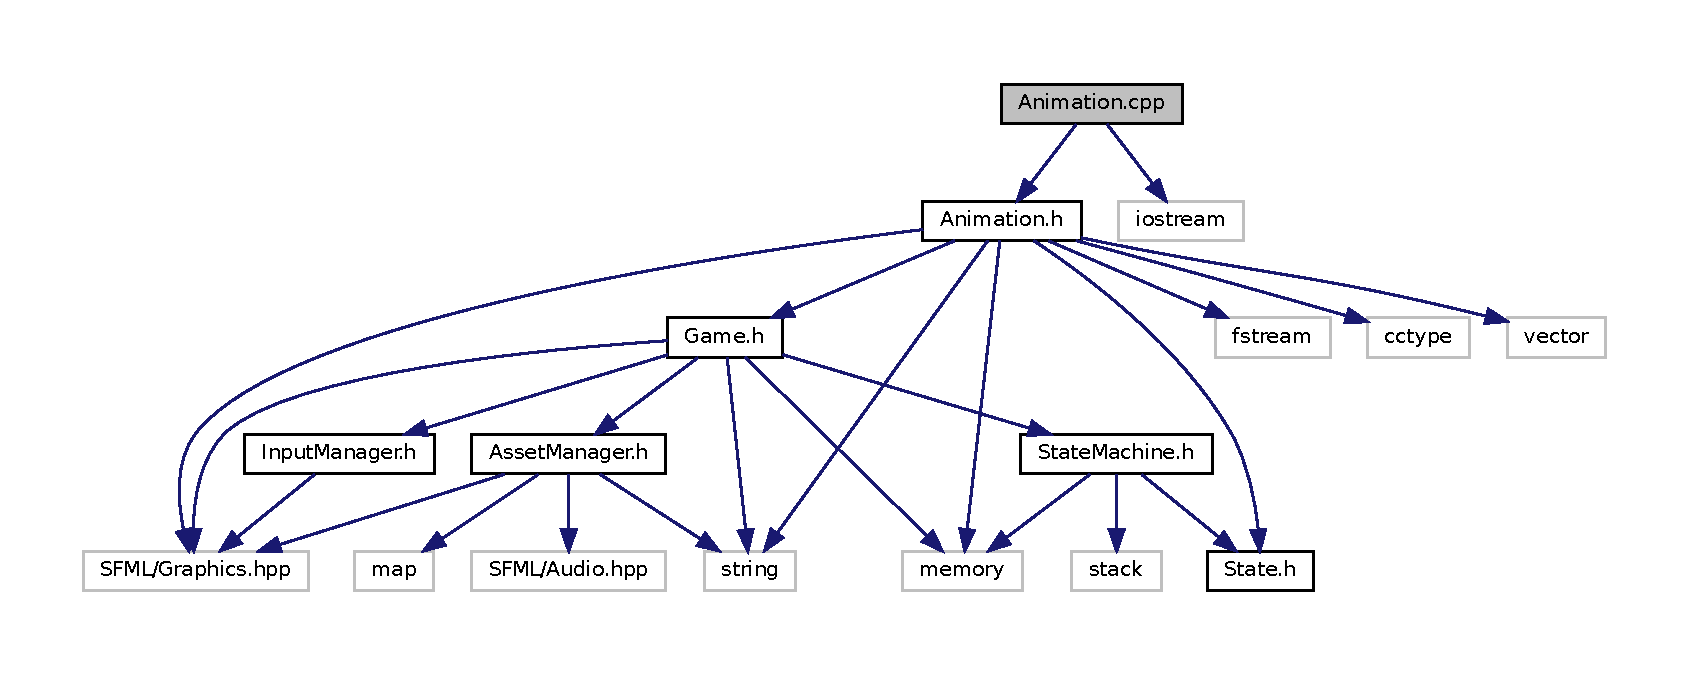
\includegraphics[width=350pt]{Animation_8cpp__incl}
\end{center}
\end{figure}

\hypertarget{Animation_8h}{}\section{Animation.\+h File Reference}
\label{Animation_8h}\index{Animation.\+h@{Animation.\+h}}
{\ttfamily \#include $<$S\+F\+M\+L/\+Graphics.\+hpp$>$}\newline
{\ttfamily \#include \char`\"{}Game.\+h\char`\"{}}\newline
{\ttfamily \#include \char`\"{}State.\+h\char`\"{}}\newline
{\ttfamily \#include $<$fstream$>$}\newline
{\ttfamily \#include $<$cctype$>$}\newline
{\ttfamily \#include $<$string$>$}\newline
{\ttfamily \#include $<$vector$>$}\newline
{\ttfamily \#include $<$memory$>$}\newline
Include dependency graph for Animation.\+h\+:\nopagebreak
\begin{figure}[H]
\begin{center}
\leavevmode
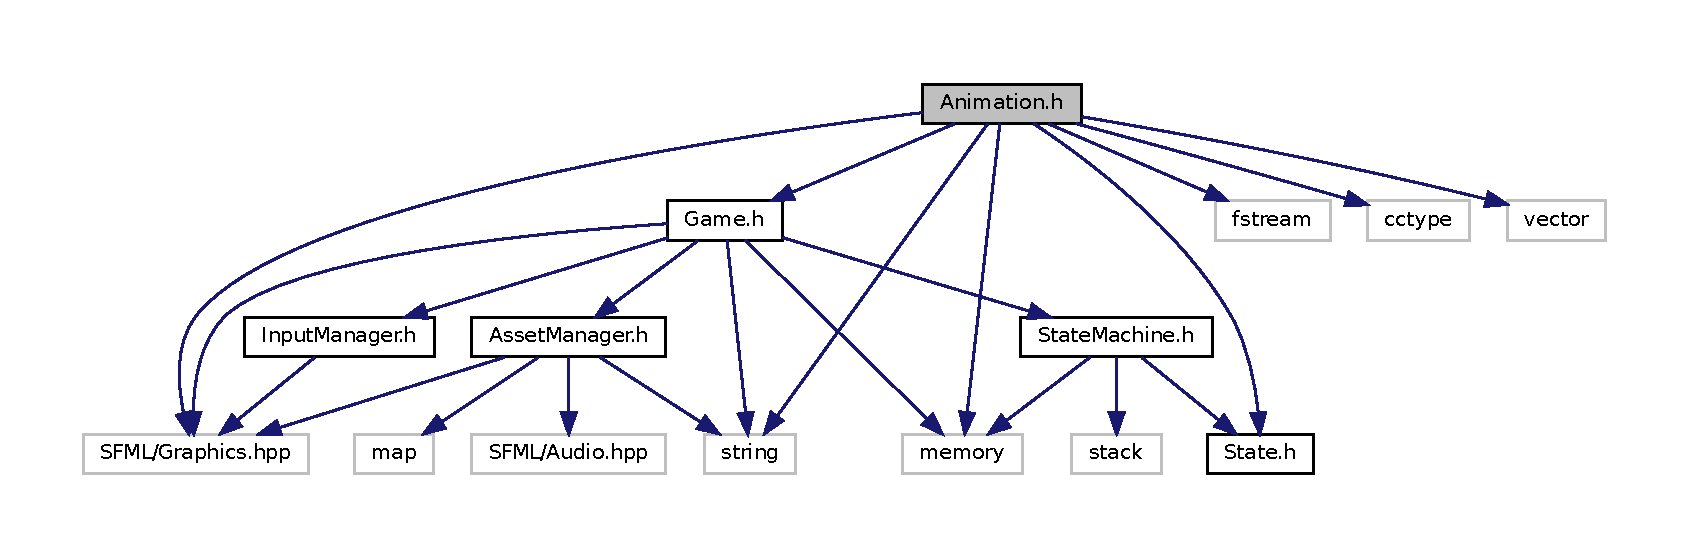
\includegraphics[width=350pt]{Animation_8h__incl}
\end{center}
\end{figure}
This graph shows which files directly or indirectly include this file\+:\nopagebreak
\begin{figure}[H]
\begin{center}
\leavevmode
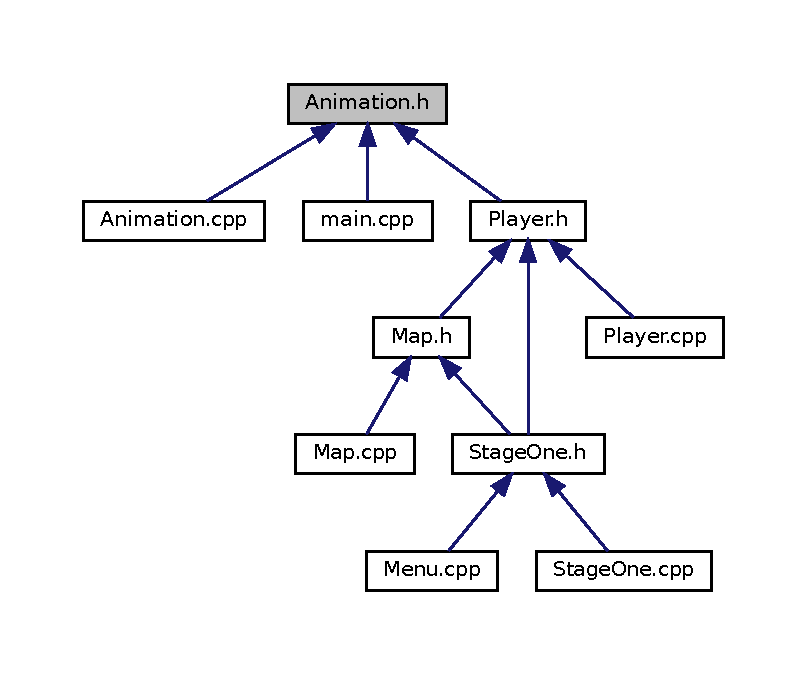
\includegraphics[width=350pt]{Animation_8h__dep__incl}
\end{center}
\end{figure}
\subsection*{Classes}
\begin{DoxyCompactItemize}
\item 
class \mbox{\hyperlink{classAnimation}{Animation}}
\end{DoxyCompactItemize}
\subsection*{Macros}
\begin{DoxyCompactItemize}
\item 
\#define \mbox{\hyperlink{Animation_8h_a1befbcd7804e879b6779d2daf1f74f7e}{A\+N\+I\+M\+A\+T\+I\+O\+N\+\_\+h}}
\end{DoxyCompactItemize}


\subsection{Macro Definition Documentation}
\mbox{\Hypertarget{Animation_8h_a1befbcd7804e879b6779d2daf1f74f7e}\label{Animation_8h_a1befbcd7804e879b6779d2daf1f74f7e}} 
\index{Animation.\+h@{Animation.\+h}!A\+N\+I\+M\+A\+T\+I\+O\+N\+\_\+h@{A\+N\+I\+M\+A\+T\+I\+O\+N\+\_\+h}}
\index{A\+N\+I\+M\+A\+T\+I\+O\+N\+\_\+h@{A\+N\+I\+M\+A\+T\+I\+O\+N\+\_\+h}!Animation.\+h@{Animation.\+h}}
\subsubsection{\texorpdfstring{A\+N\+I\+M\+A\+T\+I\+O\+N\+\_\+h}{ANIMATION\_h}}
{\footnotesize\ttfamily \#define A\+N\+I\+M\+A\+T\+I\+O\+N\+\_\+h}


\hypertarget{AssetManager_8cpp}{}\section{Asset\+Manager.\+cpp File Reference}
\label{AssetManager_8cpp}\index{Asset\+Manager.\+cpp@{Asset\+Manager.\+cpp}}
{\ttfamily \#include \char`\"{}Asset\+Manager.\+h\char`\"{}}\newline
Include dependency graph for Asset\+Manager.\+cpp\+:\nopagebreak
\begin{figure}[H]
\begin{center}
\leavevmode
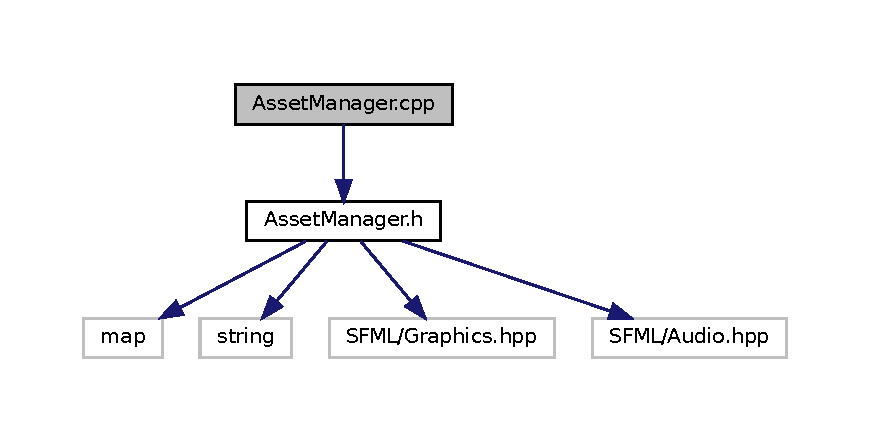
\includegraphics[width=350pt]{AssetManager_8cpp__incl}
\end{center}
\end{figure}

\hypertarget{AssetManager_8h}{}\section{Asset\+Manager.\+h File Reference}
\label{AssetManager_8h}\index{Asset\+Manager.\+h@{Asset\+Manager.\+h}}
{\ttfamily \#include $<$map$>$}\newline
{\ttfamily \#include $<$string$>$}\newline
{\ttfamily \#include $<$S\+F\+M\+L/\+Graphics.\+hpp$>$}\newline
{\ttfamily \#include $<$S\+F\+M\+L/\+Audio.\+hpp$>$}\newline
Include dependency graph for Asset\+Manager.\+h\+:\nopagebreak
\begin{figure}[H]
\begin{center}
\leavevmode
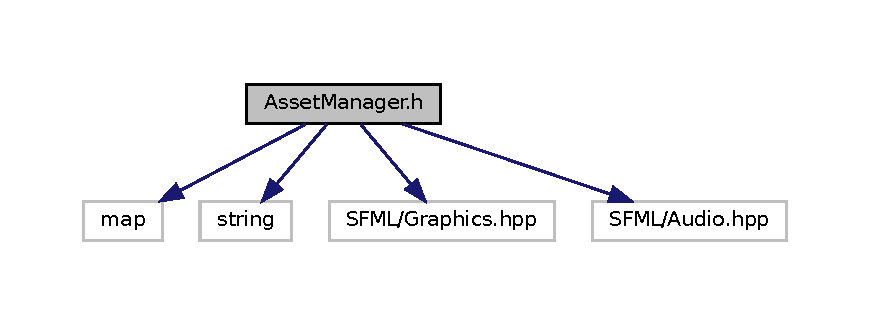
\includegraphics[width=350pt]{AssetManager_8h__incl}
\end{center}
\end{figure}
This graph shows which files directly or indirectly include this file\+:\nopagebreak
\begin{figure}[H]
\begin{center}
\leavevmode
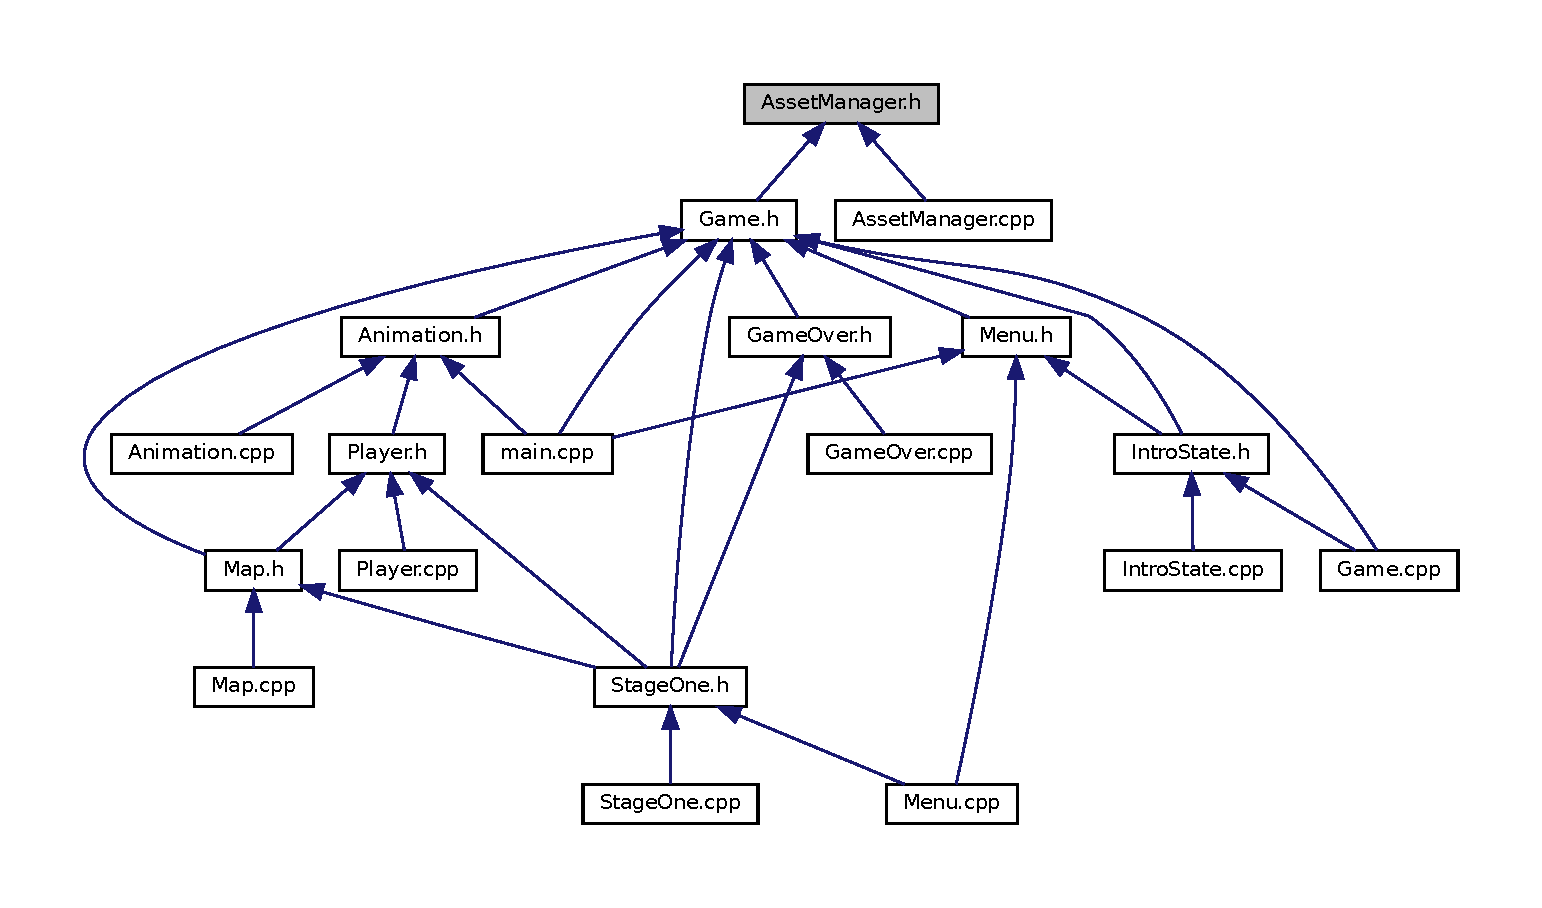
\includegraphics[width=350pt]{AssetManager_8h__dep__incl}
\end{center}
\end{figure}
\subsection*{Classes}
\begin{DoxyCompactItemize}
\item 
class \mbox{\hyperlink{classAssetManager}{Asset\+Manager}}
\end{DoxyCompactItemize}

\hypertarget{DEFINITIONS_8h}{}\section{D\+E\+F\+I\+N\+I\+T\+I\+O\+N\+S.\+h File Reference}
\label{DEFINITIONS_8h}\index{D\+E\+F\+I\+N\+I\+T\+I\+O\+N\+S.\+h@{D\+E\+F\+I\+N\+I\+T\+I\+O\+N\+S.\+h}}
This graph shows which files directly or indirectly include this file\+:\nopagebreak
\begin{figure}[H]
\begin{center}
\leavevmode
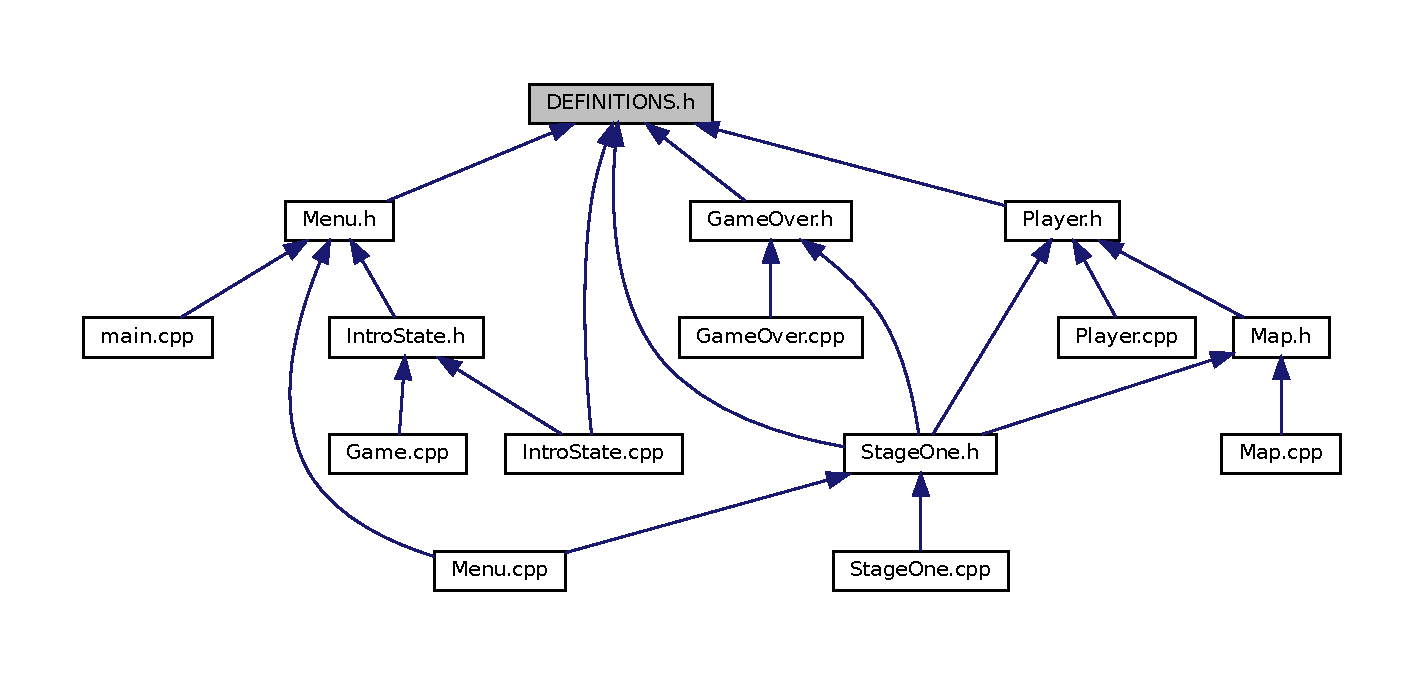
\includegraphics[width=350pt]{DEFINITIONS_8h__dep__incl}
\end{center}
\end{figure}
\subsection*{Macros}
\begin{DoxyCompactItemize}
\item 
\#define \mbox{\hyperlink{DEFINITIONS_8h_abd6e4994c3bfd3ef8328b1a98f911856}{S\+P\+L\+A\+S\+H\+\_\+\+T\+I\+M\+ER}}~3.\+0f
\item 
\#define \mbox{\hyperlink{DEFINITIONS_8h_aed91f32cb71ddf29a9d0efa0b3852ec1}{I\+N\+T\+R\+O\+\_\+\+F\+I\+L\+E\+P\+A\+TH}}~\char`\"{}tripaloski-\/splash.\+png\char`\"{}
\item 
\#define \mbox{\hyperlink{DEFINITIONS_8h_a2cd109632a6dcccaa80b43561b1ab700}{S\+C\+R\+E\+E\+N\+\_\+\+W\+I\+D\+TH}}~1024
\item 
\#define \mbox{\hyperlink{DEFINITIONS_8h_a6974d08a74da681b3957b2fead2608b8}{S\+C\+R\+E\+E\+N\+\_\+\+H\+E\+I\+G\+HT}}~768
\item 
\#define \mbox{\hyperlink{DEFINITIONS_8h_a88077b148122bd0269aa8b2a4c94aa83}{I\+N\+T\+R\+O\+\_\+\+S\+T\+A\+T\+E\+\_\+\+S\+H\+O\+W\+T\+I\+ME}}~2.\+0
\item 
\#define \mbox{\hyperlink{DEFINITIONS_8h_a71f0c59ab58cb44e61d09bb7eec6b9aa}{M\+E\+N\+U\+\_\+\+B\+A\+C\+K\+G\+R\+O\+U\+N\+D\+\_\+\+F\+I\+L\+E\+P\+A\+TH}}~\char`\"{}menu.\+png\char`\"{}
\item 
\#define \mbox{\hyperlink{DEFINITIONS_8h_ae522dd0ecdf21fe585e5b033e78b019f}{P\+L\+A\+Y\+\_\+\+B\+U\+T\+T\+O\+N\+\_\+\+F\+I\+L\+E\+P\+A\+TH}}~\char`\"{}button.\+png\char`\"{}
\item 
\#define \mbox{\hyperlink{DEFINITIONS_8h_a7e46d360b7030f48d61091b2113abdb1}{T\+I\+T\+L\+E\+\_\+\+F\+I\+L\+E\+P\+A\+TH}}~\char`\"{}B\+I\+G\+B\+O\+Y\+R\+U\+N\+N\+E\+R.\+png\char`\"{}
\item 
\#define \mbox{\hyperlink{DEFINITIONS_8h_a76108891dc4352082a676f2978ee446d}{T\+I\+L\+E\+\_\+\+W\+I\+D\+TH}}~32
\end{DoxyCompactItemize}


\subsection{Macro Definition Documentation}
\mbox{\Hypertarget{DEFINITIONS_8h_aed91f32cb71ddf29a9d0efa0b3852ec1}\label{DEFINITIONS_8h_aed91f32cb71ddf29a9d0efa0b3852ec1}} 
\index{D\+E\+F\+I\+N\+I\+T\+I\+O\+N\+S.\+h@{D\+E\+F\+I\+N\+I\+T\+I\+O\+N\+S.\+h}!I\+N\+T\+R\+O\+\_\+\+F\+I\+L\+E\+P\+A\+TH@{I\+N\+T\+R\+O\+\_\+\+F\+I\+L\+E\+P\+A\+TH}}
\index{I\+N\+T\+R\+O\+\_\+\+F\+I\+L\+E\+P\+A\+TH@{I\+N\+T\+R\+O\+\_\+\+F\+I\+L\+E\+P\+A\+TH}!D\+E\+F\+I\+N\+I\+T\+I\+O\+N\+S.\+h@{D\+E\+F\+I\+N\+I\+T\+I\+O\+N\+S.\+h}}
\subsubsection{\texorpdfstring{I\+N\+T\+R\+O\+\_\+\+F\+I\+L\+E\+P\+A\+TH}{INTRO\_FILEPATH}}
{\footnotesize\ttfamily \#define I\+N\+T\+R\+O\+\_\+\+F\+I\+L\+E\+P\+A\+TH~\char`\"{}tripaloski-\/splash.\+png\char`\"{}}

\mbox{\Hypertarget{DEFINITIONS_8h_a88077b148122bd0269aa8b2a4c94aa83}\label{DEFINITIONS_8h_a88077b148122bd0269aa8b2a4c94aa83}} 
\index{D\+E\+F\+I\+N\+I\+T\+I\+O\+N\+S.\+h@{D\+E\+F\+I\+N\+I\+T\+I\+O\+N\+S.\+h}!I\+N\+T\+R\+O\+\_\+\+S\+T\+A\+T\+E\+\_\+\+S\+H\+O\+W\+T\+I\+ME@{I\+N\+T\+R\+O\+\_\+\+S\+T\+A\+T\+E\+\_\+\+S\+H\+O\+W\+T\+I\+ME}}
\index{I\+N\+T\+R\+O\+\_\+\+S\+T\+A\+T\+E\+\_\+\+S\+H\+O\+W\+T\+I\+ME@{I\+N\+T\+R\+O\+\_\+\+S\+T\+A\+T\+E\+\_\+\+S\+H\+O\+W\+T\+I\+ME}!D\+E\+F\+I\+N\+I\+T\+I\+O\+N\+S.\+h@{D\+E\+F\+I\+N\+I\+T\+I\+O\+N\+S.\+h}}
\subsubsection{\texorpdfstring{I\+N\+T\+R\+O\+\_\+\+S\+T\+A\+T\+E\+\_\+\+S\+H\+O\+W\+T\+I\+ME}{INTRO\_STATE\_SHOWTIME}}
{\footnotesize\ttfamily \#define I\+N\+T\+R\+O\+\_\+\+S\+T\+A\+T\+E\+\_\+\+S\+H\+O\+W\+T\+I\+ME~2.\+0}

\mbox{\Hypertarget{DEFINITIONS_8h_a71f0c59ab58cb44e61d09bb7eec6b9aa}\label{DEFINITIONS_8h_a71f0c59ab58cb44e61d09bb7eec6b9aa}} 
\index{D\+E\+F\+I\+N\+I\+T\+I\+O\+N\+S.\+h@{D\+E\+F\+I\+N\+I\+T\+I\+O\+N\+S.\+h}!M\+E\+N\+U\+\_\+\+B\+A\+C\+K\+G\+R\+O\+U\+N\+D\+\_\+\+F\+I\+L\+E\+P\+A\+TH@{M\+E\+N\+U\+\_\+\+B\+A\+C\+K\+G\+R\+O\+U\+N\+D\+\_\+\+F\+I\+L\+E\+P\+A\+TH}}
\index{M\+E\+N\+U\+\_\+\+B\+A\+C\+K\+G\+R\+O\+U\+N\+D\+\_\+\+F\+I\+L\+E\+P\+A\+TH@{M\+E\+N\+U\+\_\+\+B\+A\+C\+K\+G\+R\+O\+U\+N\+D\+\_\+\+F\+I\+L\+E\+P\+A\+TH}!D\+E\+F\+I\+N\+I\+T\+I\+O\+N\+S.\+h@{D\+E\+F\+I\+N\+I\+T\+I\+O\+N\+S.\+h}}
\subsubsection{\texorpdfstring{M\+E\+N\+U\+\_\+\+B\+A\+C\+K\+G\+R\+O\+U\+N\+D\+\_\+\+F\+I\+L\+E\+P\+A\+TH}{MENU\_BACKGROUND\_FILEPATH}}
{\footnotesize\ttfamily \#define M\+E\+N\+U\+\_\+\+B\+A\+C\+K\+G\+R\+O\+U\+N\+D\+\_\+\+F\+I\+L\+E\+P\+A\+TH~\char`\"{}menu.\+png\char`\"{}}

\mbox{\Hypertarget{DEFINITIONS_8h_ae522dd0ecdf21fe585e5b033e78b019f}\label{DEFINITIONS_8h_ae522dd0ecdf21fe585e5b033e78b019f}} 
\index{D\+E\+F\+I\+N\+I\+T\+I\+O\+N\+S.\+h@{D\+E\+F\+I\+N\+I\+T\+I\+O\+N\+S.\+h}!P\+L\+A\+Y\+\_\+\+B\+U\+T\+T\+O\+N\+\_\+\+F\+I\+L\+E\+P\+A\+TH@{P\+L\+A\+Y\+\_\+\+B\+U\+T\+T\+O\+N\+\_\+\+F\+I\+L\+E\+P\+A\+TH}}
\index{P\+L\+A\+Y\+\_\+\+B\+U\+T\+T\+O\+N\+\_\+\+F\+I\+L\+E\+P\+A\+TH@{P\+L\+A\+Y\+\_\+\+B\+U\+T\+T\+O\+N\+\_\+\+F\+I\+L\+E\+P\+A\+TH}!D\+E\+F\+I\+N\+I\+T\+I\+O\+N\+S.\+h@{D\+E\+F\+I\+N\+I\+T\+I\+O\+N\+S.\+h}}
\subsubsection{\texorpdfstring{P\+L\+A\+Y\+\_\+\+B\+U\+T\+T\+O\+N\+\_\+\+F\+I\+L\+E\+P\+A\+TH}{PLAY\_BUTTON\_FILEPATH}}
{\footnotesize\ttfamily \#define P\+L\+A\+Y\+\_\+\+B\+U\+T\+T\+O\+N\+\_\+\+F\+I\+L\+E\+P\+A\+TH~\char`\"{}button.\+png\char`\"{}}

\mbox{\Hypertarget{DEFINITIONS_8h_a6974d08a74da681b3957b2fead2608b8}\label{DEFINITIONS_8h_a6974d08a74da681b3957b2fead2608b8}} 
\index{D\+E\+F\+I\+N\+I\+T\+I\+O\+N\+S.\+h@{D\+E\+F\+I\+N\+I\+T\+I\+O\+N\+S.\+h}!S\+C\+R\+E\+E\+N\+\_\+\+H\+E\+I\+G\+HT@{S\+C\+R\+E\+E\+N\+\_\+\+H\+E\+I\+G\+HT}}
\index{S\+C\+R\+E\+E\+N\+\_\+\+H\+E\+I\+G\+HT@{S\+C\+R\+E\+E\+N\+\_\+\+H\+E\+I\+G\+HT}!D\+E\+F\+I\+N\+I\+T\+I\+O\+N\+S.\+h@{D\+E\+F\+I\+N\+I\+T\+I\+O\+N\+S.\+h}}
\subsubsection{\texorpdfstring{S\+C\+R\+E\+E\+N\+\_\+\+H\+E\+I\+G\+HT}{SCREEN\_HEIGHT}}
{\footnotesize\ttfamily \#define S\+C\+R\+E\+E\+N\+\_\+\+H\+E\+I\+G\+HT~768}

\mbox{\Hypertarget{DEFINITIONS_8h_a2cd109632a6dcccaa80b43561b1ab700}\label{DEFINITIONS_8h_a2cd109632a6dcccaa80b43561b1ab700}} 
\index{D\+E\+F\+I\+N\+I\+T\+I\+O\+N\+S.\+h@{D\+E\+F\+I\+N\+I\+T\+I\+O\+N\+S.\+h}!S\+C\+R\+E\+E\+N\+\_\+\+W\+I\+D\+TH@{S\+C\+R\+E\+E\+N\+\_\+\+W\+I\+D\+TH}}
\index{S\+C\+R\+E\+E\+N\+\_\+\+W\+I\+D\+TH@{S\+C\+R\+E\+E\+N\+\_\+\+W\+I\+D\+TH}!D\+E\+F\+I\+N\+I\+T\+I\+O\+N\+S.\+h@{D\+E\+F\+I\+N\+I\+T\+I\+O\+N\+S.\+h}}
\subsubsection{\texorpdfstring{S\+C\+R\+E\+E\+N\+\_\+\+W\+I\+D\+TH}{SCREEN\_WIDTH}}
{\footnotesize\ttfamily \#define S\+C\+R\+E\+E\+N\+\_\+\+W\+I\+D\+TH~1024}

\mbox{\Hypertarget{DEFINITIONS_8h_abd6e4994c3bfd3ef8328b1a98f911856}\label{DEFINITIONS_8h_abd6e4994c3bfd3ef8328b1a98f911856}} 
\index{D\+E\+F\+I\+N\+I\+T\+I\+O\+N\+S.\+h@{D\+E\+F\+I\+N\+I\+T\+I\+O\+N\+S.\+h}!S\+P\+L\+A\+S\+H\+\_\+\+T\+I\+M\+ER@{S\+P\+L\+A\+S\+H\+\_\+\+T\+I\+M\+ER}}
\index{S\+P\+L\+A\+S\+H\+\_\+\+T\+I\+M\+ER@{S\+P\+L\+A\+S\+H\+\_\+\+T\+I\+M\+ER}!D\+E\+F\+I\+N\+I\+T\+I\+O\+N\+S.\+h@{D\+E\+F\+I\+N\+I\+T\+I\+O\+N\+S.\+h}}
\subsubsection{\texorpdfstring{S\+P\+L\+A\+S\+H\+\_\+\+T\+I\+M\+ER}{SPLASH\_TIMER}}
{\footnotesize\ttfamily \#define S\+P\+L\+A\+S\+H\+\_\+\+T\+I\+M\+ER~3.\+0f}

\mbox{\Hypertarget{DEFINITIONS_8h_a76108891dc4352082a676f2978ee446d}\label{DEFINITIONS_8h_a76108891dc4352082a676f2978ee446d}} 
\index{D\+E\+F\+I\+N\+I\+T\+I\+O\+N\+S.\+h@{D\+E\+F\+I\+N\+I\+T\+I\+O\+N\+S.\+h}!T\+I\+L\+E\+\_\+\+W\+I\+D\+TH@{T\+I\+L\+E\+\_\+\+W\+I\+D\+TH}}
\index{T\+I\+L\+E\+\_\+\+W\+I\+D\+TH@{T\+I\+L\+E\+\_\+\+W\+I\+D\+TH}!D\+E\+F\+I\+N\+I\+T\+I\+O\+N\+S.\+h@{D\+E\+F\+I\+N\+I\+T\+I\+O\+N\+S.\+h}}
\subsubsection{\texorpdfstring{T\+I\+L\+E\+\_\+\+W\+I\+D\+TH}{TILE\_WIDTH}}
{\footnotesize\ttfamily \#define T\+I\+L\+E\+\_\+\+W\+I\+D\+TH~32}

\mbox{\Hypertarget{DEFINITIONS_8h_a7e46d360b7030f48d61091b2113abdb1}\label{DEFINITIONS_8h_a7e46d360b7030f48d61091b2113abdb1}} 
\index{D\+E\+F\+I\+N\+I\+T\+I\+O\+N\+S.\+h@{D\+E\+F\+I\+N\+I\+T\+I\+O\+N\+S.\+h}!T\+I\+T\+L\+E\+\_\+\+F\+I\+L\+E\+P\+A\+TH@{T\+I\+T\+L\+E\+\_\+\+F\+I\+L\+E\+P\+A\+TH}}
\index{T\+I\+T\+L\+E\+\_\+\+F\+I\+L\+E\+P\+A\+TH@{T\+I\+T\+L\+E\+\_\+\+F\+I\+L\+E\+P\+A\+TH}!D\+E\+F\+I\+N\+I\+T\+I\+O\+N\+S.\+h@{D\+E\+F\+I\+N\+I\+T\+I\+O\+N\+S.\+h}}
\subsubsection{\texorpdfstring{T\+I\+T\+L\+E\+\_\+\+F\+I\+L\+E\+P\+A\+TH}{TITLE\_FILEPATH}}
{\footnotesize\ttfamily \#define T\+I\+T\+L\+E\+\_\+\+F\+I\+L\+E\+P\+A\+TH~\char`\"{}B\+I\+G\+B\+O\+Y\+R\+U\+N\+N\+E\+R.\+png\char`\"{}}


\hypertarget{Game_8cpp}{}\section{Game.\+cpp File Reference}
\label{Game_8cpp}\index{Game.\+cpp@{Game.\+cpp}}
{\ttfamily \#include \char`\"{}Game.\+h\char`\"{}}\newline
{\ttfamily \#include \char`\"{}Intro\+State.\+h\char`\"{}}\newline
Include dependency graph for Game.\+cpp\+:\nopagebreak
\begin{figure}[H]
\begin{center}
\leavevmode
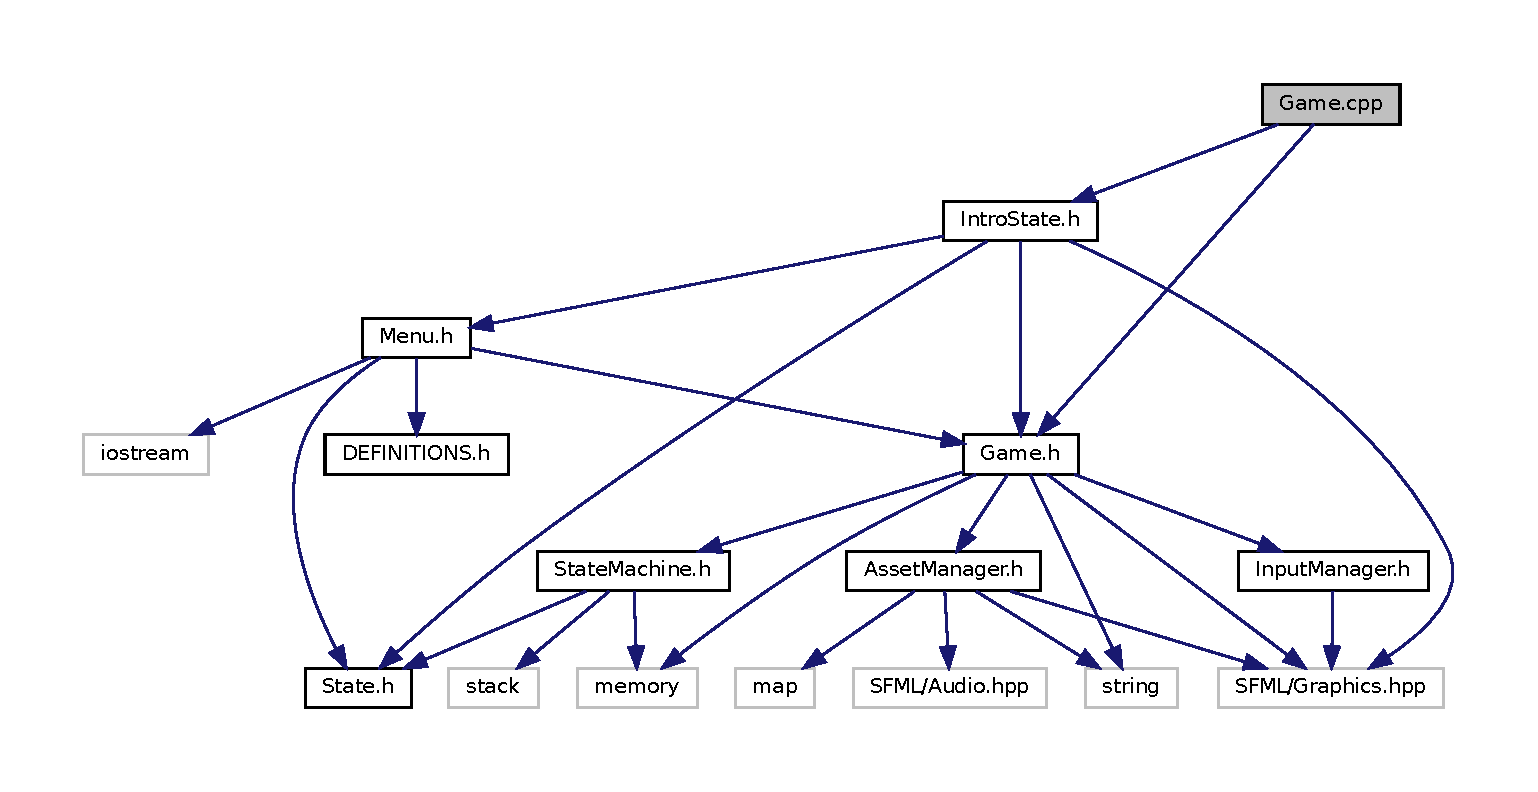
\includegraphics[width=350pt]{Game_8cpp__incl}
\end{center}
\end{figure}

\hypertarget{Game_8h}{}\section{Game.\+h File Reference}
\label{Game_8h}\index{Game.\+h@{Game.\+h}}
{\ttfamily \#include $<$memory$>$}\newline
{\ttfamily \#include $<$string$>$}\newline
{\ttfamily \#include $<$S\+F\+M\+L/\+Graphics.\+hpp$>$}\newline
{\ttfamily \#include \char`\"{}State\+Machine.\+h\char`\"{}}\newline
{\ttfamily \#include \char`\"{}Input\+Manager.\+h\char`\"{}}\newline
{\ttfamily \#include \char`\"{}Asset\+Manager.\+h\char`\"{}}\newline
Include dependency graph for Game.\+h\+:\nopagebreak
\begin{figure}[H]
\begin{center}
\leavevmode
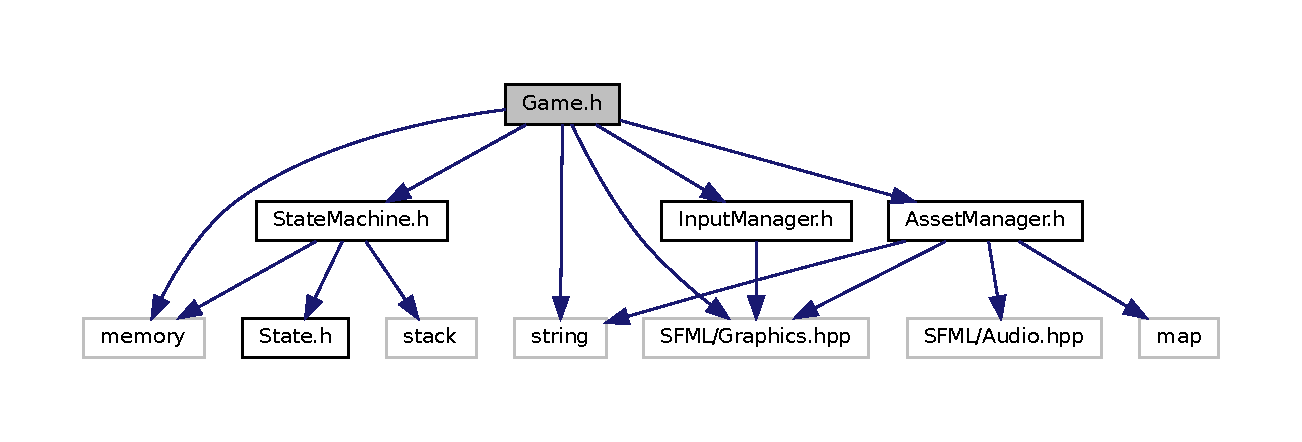
\includegraphics[width=350pt]{Game_8h__incl}
\end{center}
\end{figure}
This graph shows which files directly or indirectly include this file\+:\nopagebreak
\begin{figure}[H]
\begin{center}
\leavevmode
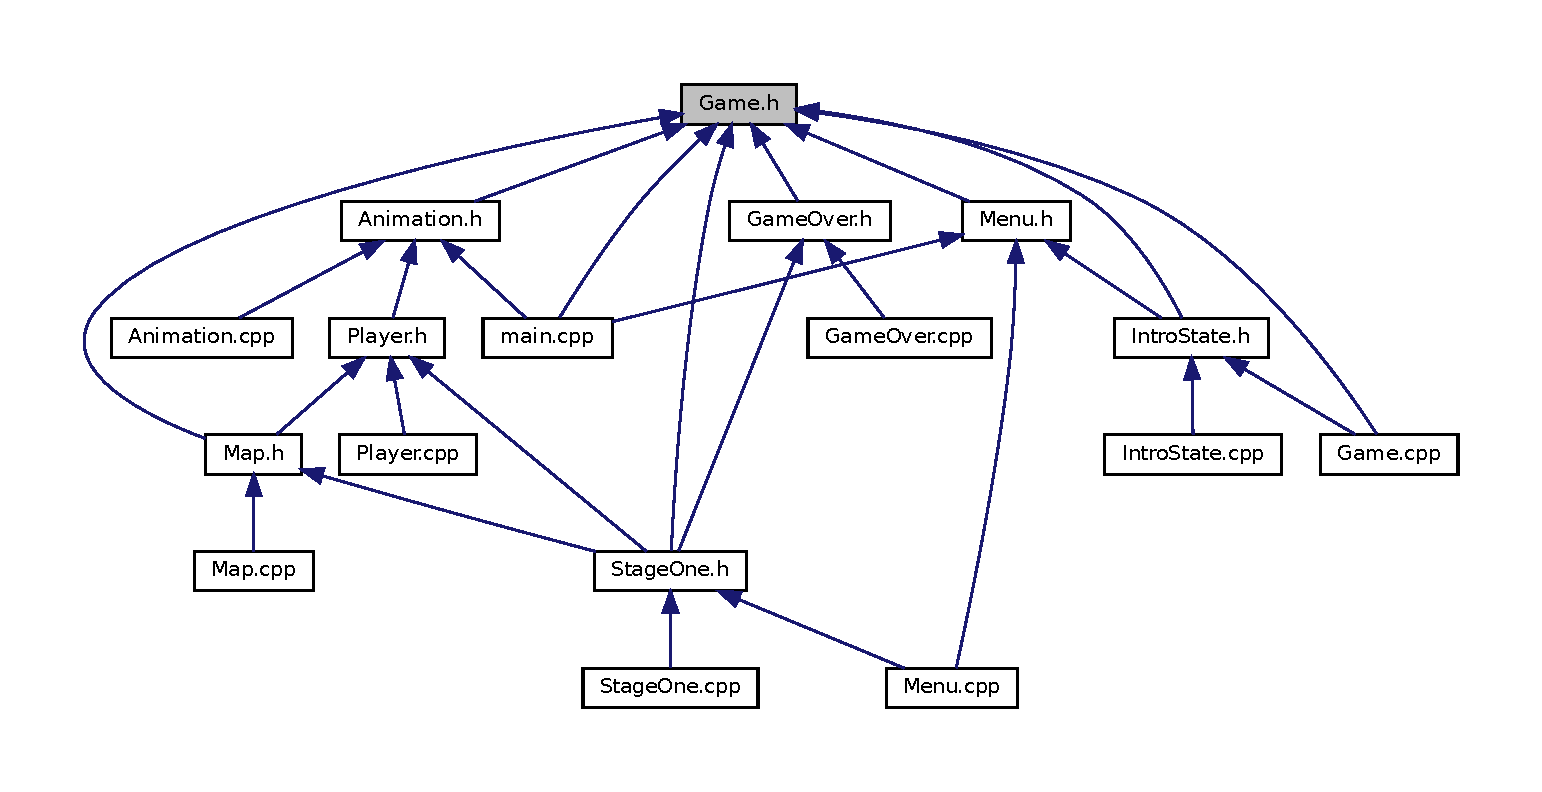
\includegraphics[width=350pt]{Game_8h__dep__incl}
\end{center}
\end{figure}
\subsection*{Classes}
\begin{DoxyCompactItemize}
\item 
struct \mbox{\hyperlink{structGameData}{Game\+Data}}
\item 
class \mbox{\hyperlink{classGame}{Game}}
\end{DoxyCompactItemize}
\subsection*{Typedefs}
\begin{DoxyCompactItemize}
\item 
typedef std\+::shared\+\_\+ptr$<$ \mbox{\hyperlink{structGameData}{Game\+Data}} $>$ \mbox{\hyperlink{Game_8h_aff850703a7797c8bfee2f02906aec50c}{Game\+Data\+Ref}}
\end{DoxyCompactItemize}


\subsection{Typedef Documentation}
\mbox{\Hypertarget{Game_8h_aff850703a7797c8bfee2f02906aec50c}\label{Game_8h_aff850703a7797c8bfee2f02906aec50c}} 
\index{Game.\+h@{Game.\+h}!Game\+Data\+Ref@{Game\+Data\+Ref}}
\index{Game\+Data\+Ref@{Game\+Data\+Ref}!Game.\+h@{Game.\+h}}
\subsubsection{\texorpdfstring{Game\+Data\+Ref}{GameDataRef}}
{\footnotesize\ttfamily typedef std\+::shared\+\_\+ptr$<$\mbox{\hyperlink{structGameData}{Game\+Data}}$>$ \mbox{\hyperlink{Game_8h_aff850703a7797c8bfee2f02906aec50c}{Game\+Data\+Ref}}}


\hypertarget{GameOver_8cpp}{}\section{Game\+Over.\+cpp File Reference}
\label{GameOver_8cpp}\index{Game\+Over.\+cpp@{Game\+Over.\+cpp}}
{\ttfamily \#include \char`\"{}Game\+Over.\+h\char`\"{}}\newline
{\ttfamily \#include $<$iostream$>$}\newline
Include dependency graph for Game\+Over.\+cpp\+:\nopagebreak
\begin{figure}[H]
\begin{center}
\leavevmode
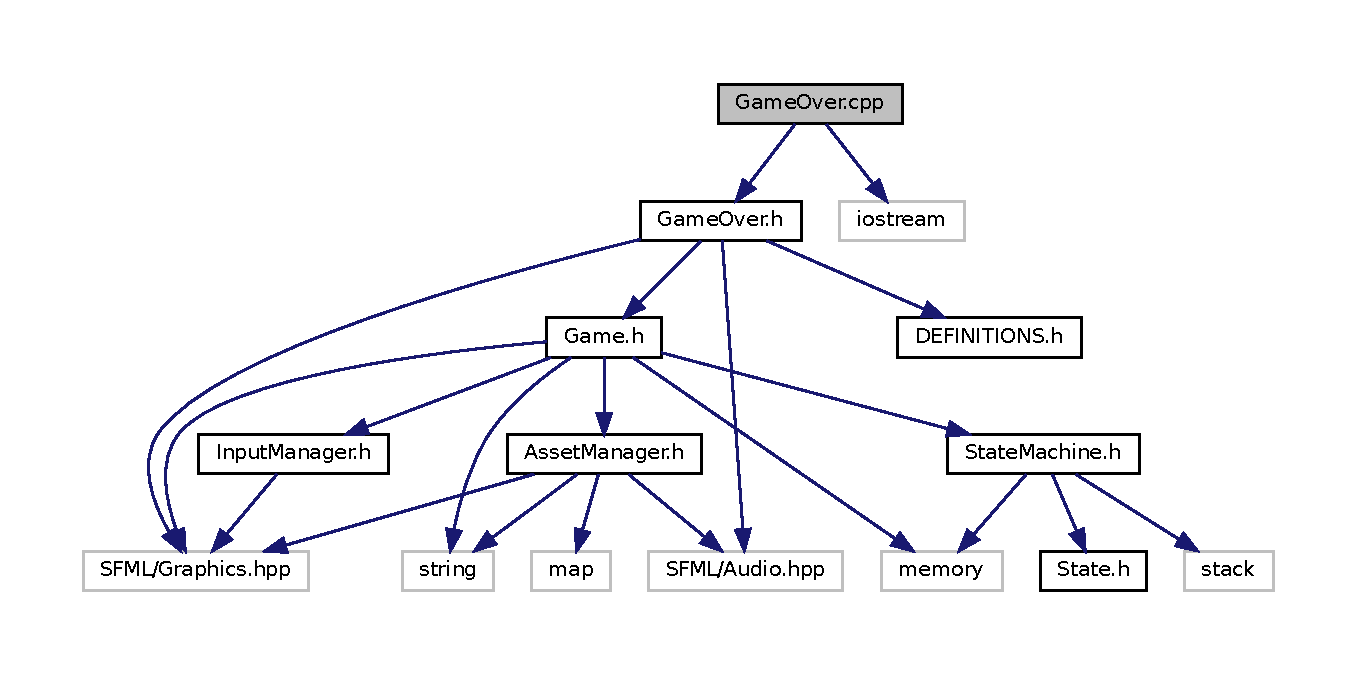
\includegraphics[width=350pt]{GameOver_8cpp__incl}
\end{center}
\end{figure}

\hypertarget{GameOver_8h}{}\section{Game\+Over.\+h File Reference}
\label{GameOver_8h}\index{Game\+Over.\+h@{Game\+Over.\+h}}
{\ttfamily \#include $<$S\+F\+M\+L/\+Graphics.\+hpp$>$}\newline
{\ttfamily \#include \char`\"{}Game.\+h\char`\"{}}\newline
{\ttfamily \#include \char`\"{}D\+E\+F\+I\+N\+I\+T\+I\+O\+N\+S.\+h\char`\"{}}\newline
{\ttfamily \#include $<$S\+F\+M\+L/\+Audio.\+hpp$>$}\newline
Include dependency graph for Game\+Over.\+h\+:\nopagebreak
\begin{figure}[H]
\begin{center}
\leavevmode
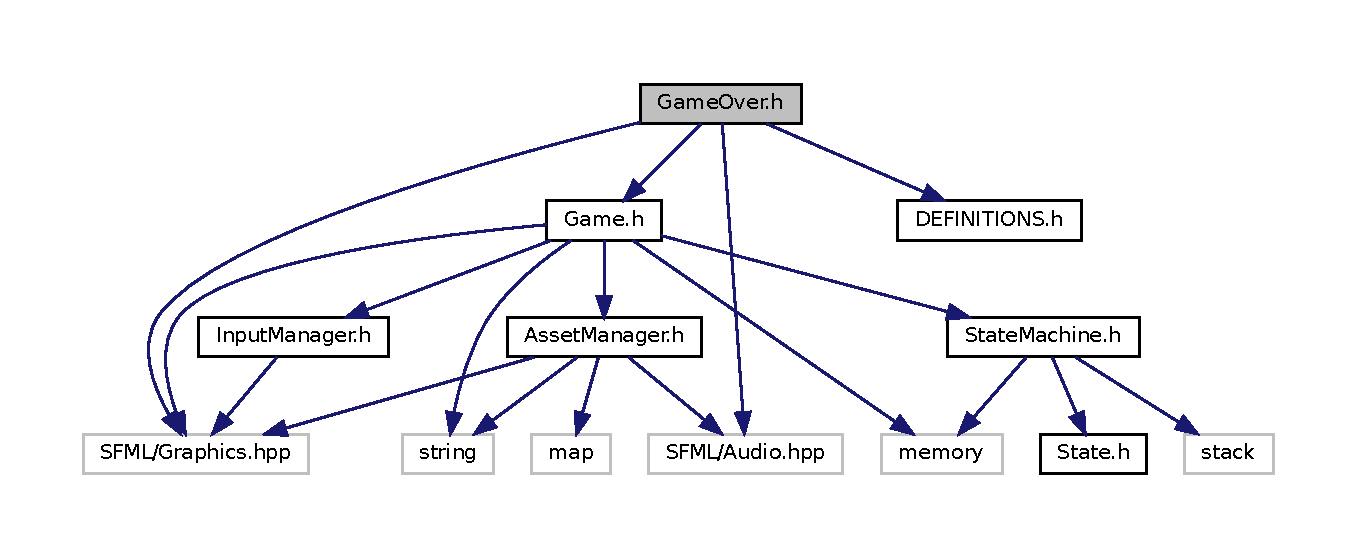
\includegraphics[width=350pt]{GameOver_8h__incl}
\end{center}
\end{figure}
This graph shows which files directly or indirectly include this file\+:\nopagebreak
\begin{figure}[H]
\begin{center}
\leavevmode
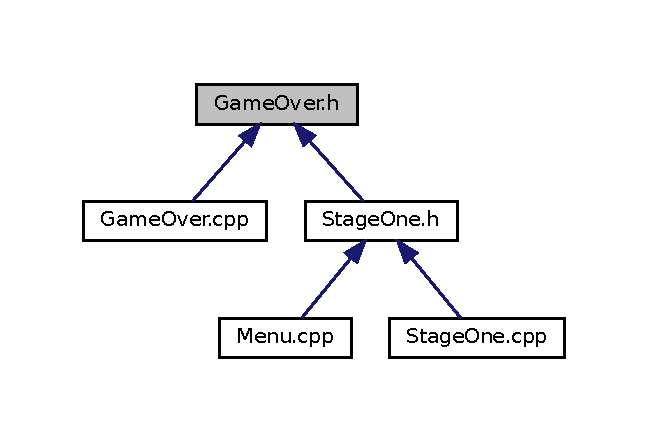
\includegraphics[width=311pt]{GameOver_8h__dep__incl}
\end{center}
\end{figure}
\subsection*{Classes}
\begin{DoxyCompactItemize}
\item 
class \mbox{\hyperlink{classGameOver}{Game\+Over}}
\end{DoxyCompactItemize}

\hypertarget{InputManager_8cpp}{}\section{Input\+Manager.\+cpp File Reference}
\label{InputManager_8cpp}\index{Input\+Manager.\+cpp@{Input\+Manager.\+cpp}}
{\ttfamily \#include \char`\"{}Input\+Manager.\+h\char`\"{}}\newline
Include dependency graph for Input\+Manager.\+cpp\+:\nopagebreak
\begin{figure}[H]
\begin{center}
\leavevmode
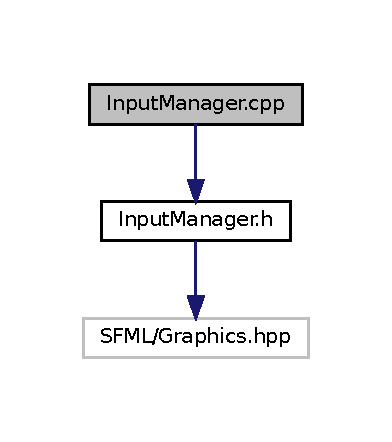
\includegraphics[width=188pt]{InputManager_8cpp__incl}
\end{center}
\end{figure}

\hypertarget{InputManager_8h}{}\section{Input\+Manager.\+h File Reference}
\label{InputManager_8h}\index{Input\+Manager.\+h@{Input\+Manager.\+h}}
{\ttfamily \#include $<$S\+F\+M\+L/\+Graphics.\+hpp$>$}\newline
Include dependency graph for Input\+Manager.\+h\+:\nopagebreak
\begin{figure}[H]
\begin{center}
\leavevmode
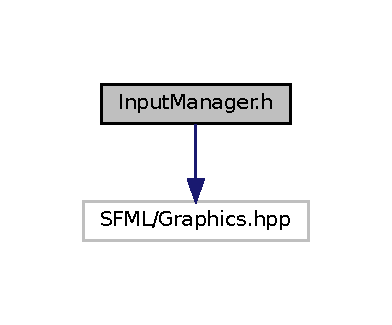
\includegraphics[width=188pt]{InputManager_8h__incl}
\end{center}
\end{figure}
This graph shows which files directly or indirectly include this file\+:\nopagebreak
\begin{figure}[H]
\begin{center}
\leavevmode
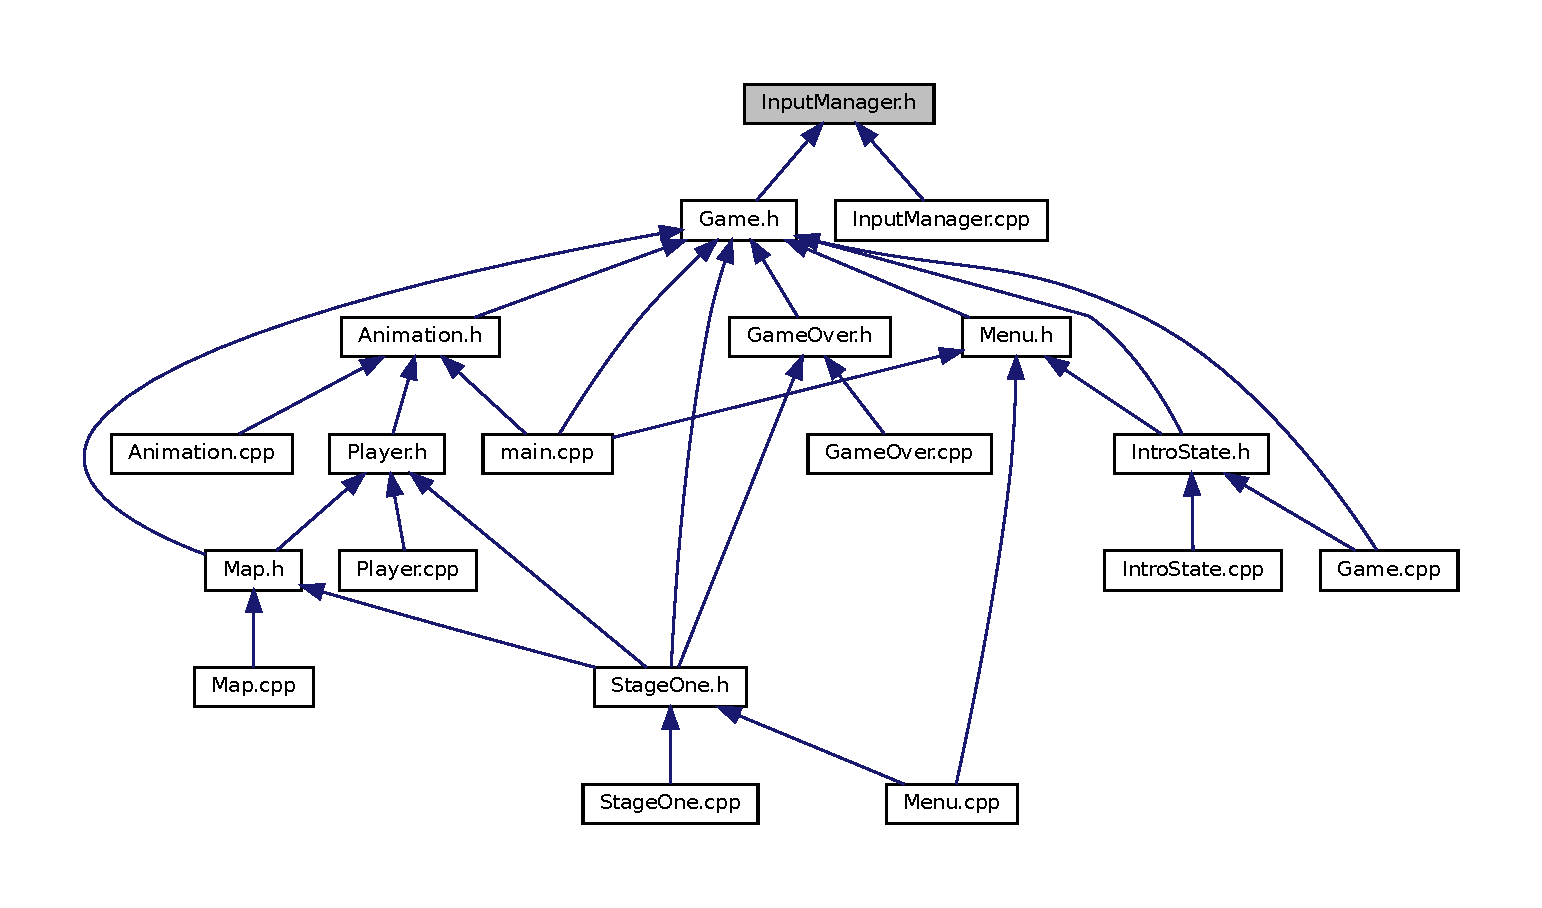
\includegraphics[width=350pt]{InputManager_8h__dep__incl}
\end{center}
\end{figure}
\subsection*{Classes}
\begin{DoxyCompactItemize}
\item 
class \mbox{\hyperlink{classInputManager}{Input\+Manager}}
\begin{DoxyCompactList}\small\item\em Gets mouse button Inputs. \end{DoxyCompactList}\end{DoxyCompactItemize}

\hypertarget{IntroState_8cpp}{}\section{Intro\+State.\+cpp File Reference}
\label{IntroState_8cpp}\index{Intro\+State.\+cpp@{Intro\+State.\+cpp}}
{\ttfamily \#include \char`\"{}Intro\+State.\+h\char`\"{}}\newline
{\ttfamily \#include \char`\"{}D\+E\+F\+I\+N\+I\+T\+I\+O\+N\+S.\+h\char`\"{}}\newline
{\ttfamily \#include $<$iostream$>$}\newline
Include dependency graph for Intro\+State.\+cpp\+:\nopagebreak
\begin{figure}[H]
\begin{center}
\leavevmode
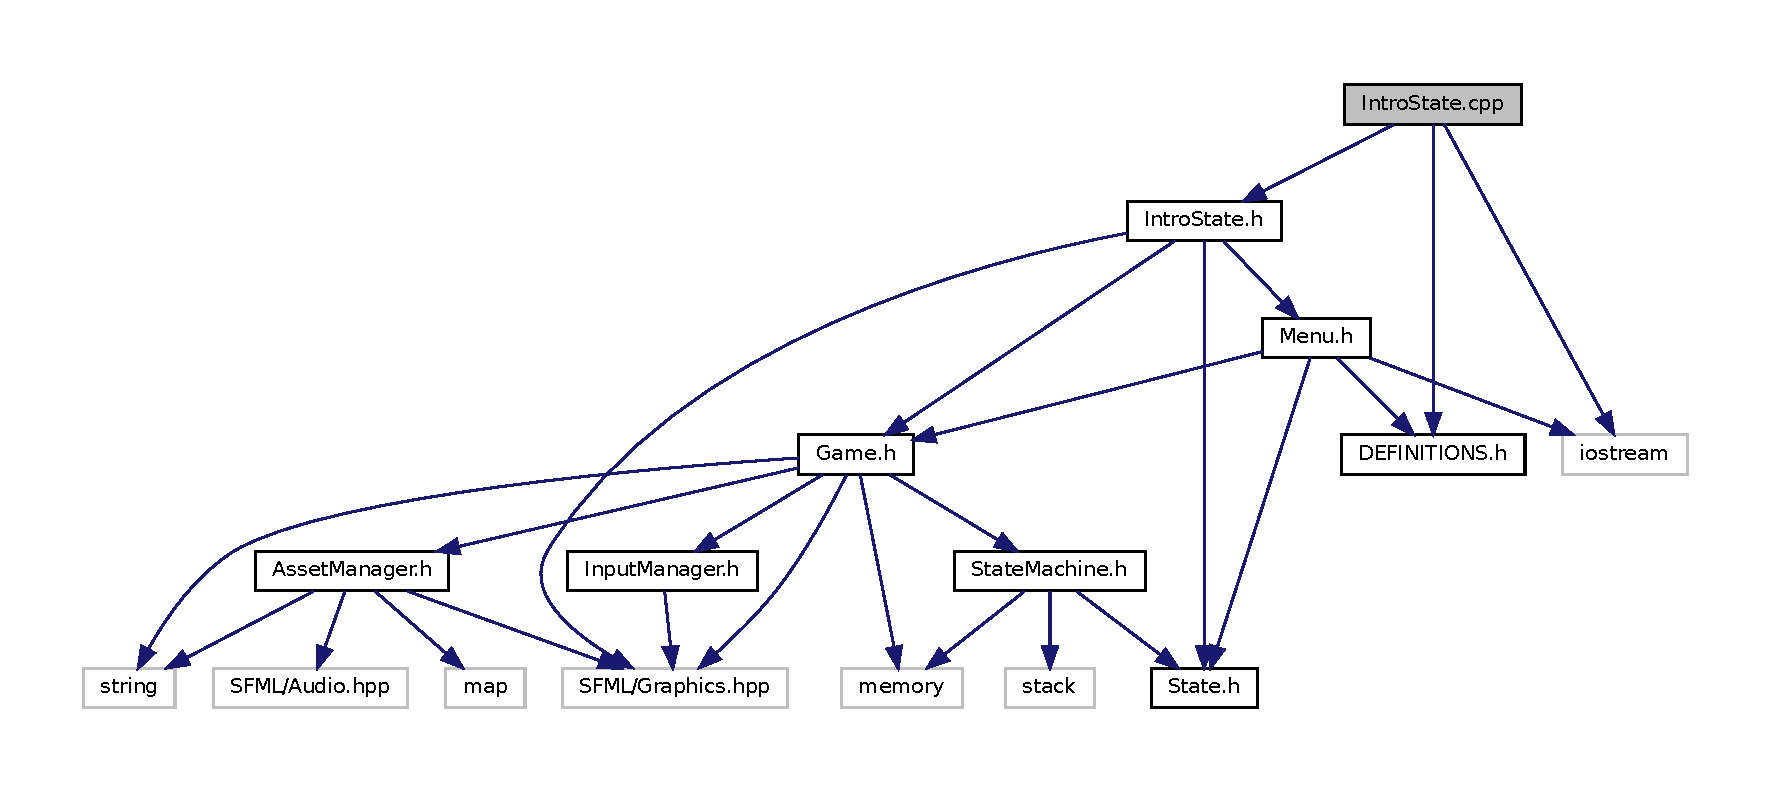
\includegraphics[width=350pt]{IntroState_8cpp__incl}
\end{center}
\end{figure}

\hypertarget{IntroState_8h}{}\section{Intro\+State.\+h File Reference}
\label{IntroState_8h}\index{Intro\+State.\+h@{Intro\+State.\+h}}
{\ttfamily \#include $<$S\+F\+M\+L/\+Graphics.\+hpp$>$}\newline
{\ttfamily \#include \char`\"{}State.\+h\char`\"{}}\newline
{\ttfamily \#include \char`\"{}Game.\+h\char`\"{}}\newline
{\ttfamily \#include \char`\"{}Menu.\+h\char`\"{}}\newline
Include dependency graph for Intro\+State.\+h\+:\nopagebreak
\begin{figure}[H]
\begin{center}
\leavevmode
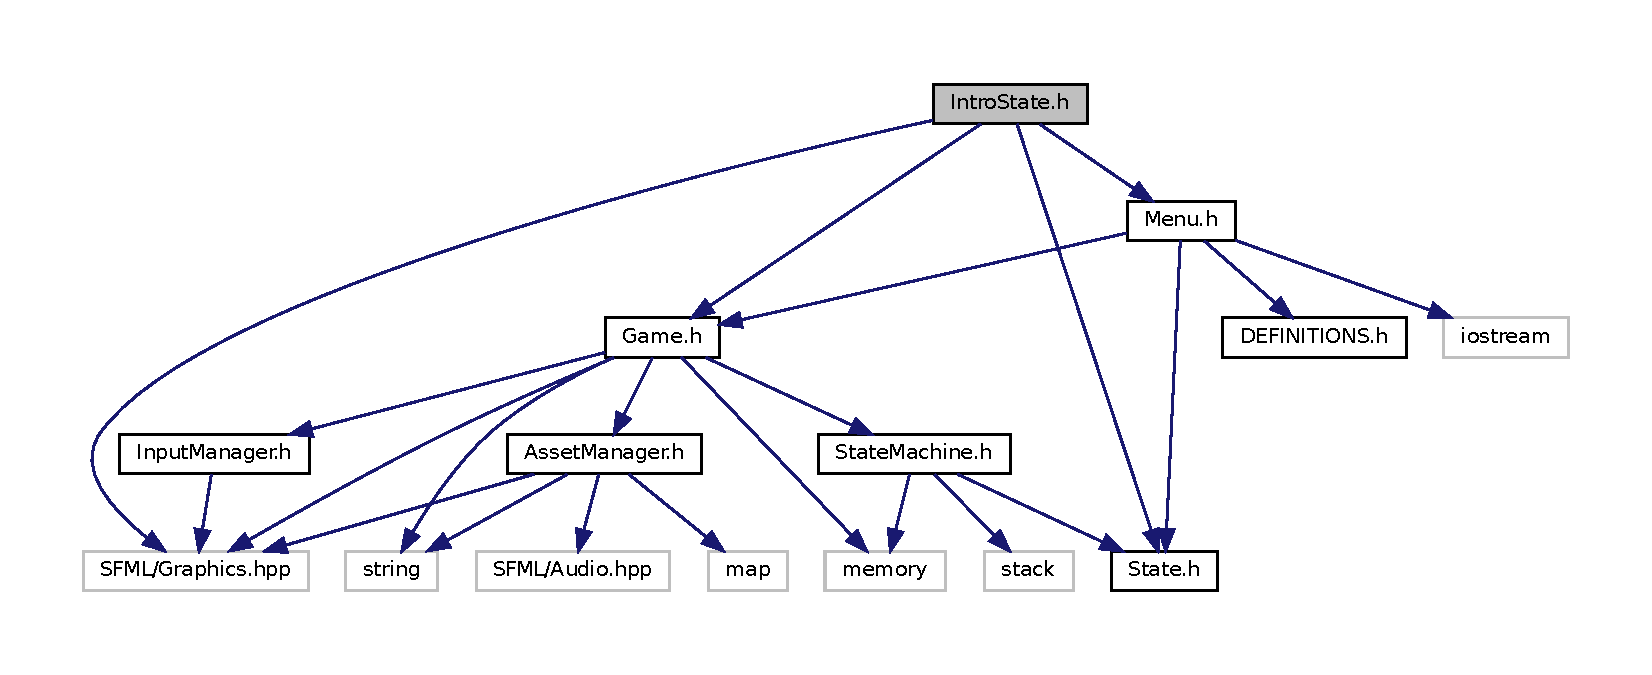
\includegraphics[width=350pt]{IntroState_8h__incl}
\end{center}
\end{figure}
This graph shows which files directly or indirectly include this file\+:\nopagebreak
\begin{figure}[H]
\begin{center}
\leavevmode
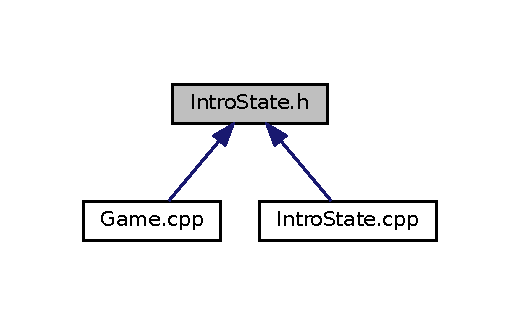
\includegraphics[width=250pt]{IntroState_8h__dep__incl}
\end{center}
\end{figure}
\subsection*{Classes}
\begin{DoxyCompactItemize}
\item 
class \mbox{\hyperlink{classIntroState}{Intro\+State}}
\end{DoxyCompactItemize}

\hypertarget{main_8cpp}{}\section{main.\+cpp File Reference}
\label{main_8cpp}\index{main.\+cpp@{main.\+cpp}}
{\ttfamily \#include $<$S\+F\+M\+L/\+Graphics.\+hpp$>$}\newline
{\ttfamily \#include $<$iostream$>$}\newline
{\ttfamily \#include \char`\"{}Animation.\+h\char`\"{}}\newline
{\ttfamily \#include \char`\"{}Game.\+h\char`\"{}}\newline
{\ttfamily \#include \char`\"{}Menu.\+h\char`\"{}}\newline
{\ttfamily \#include $<$fstream$>$}\newline
{\ttfamily \#include $<$cctype$>$}\newline
{\ttfamily \#include $<$string$>$}\newline
{\ttfamily \#include $<$vector$>$}\newline
{\ttfamily \#include $<$S\+F\+M\+L/\+Audio.\+hpp$>$}\newline
Include dependency graph for main.\+cpp\+:\nopagebreak
\begin{figure}[H]
\begin{center}
\leavevmode
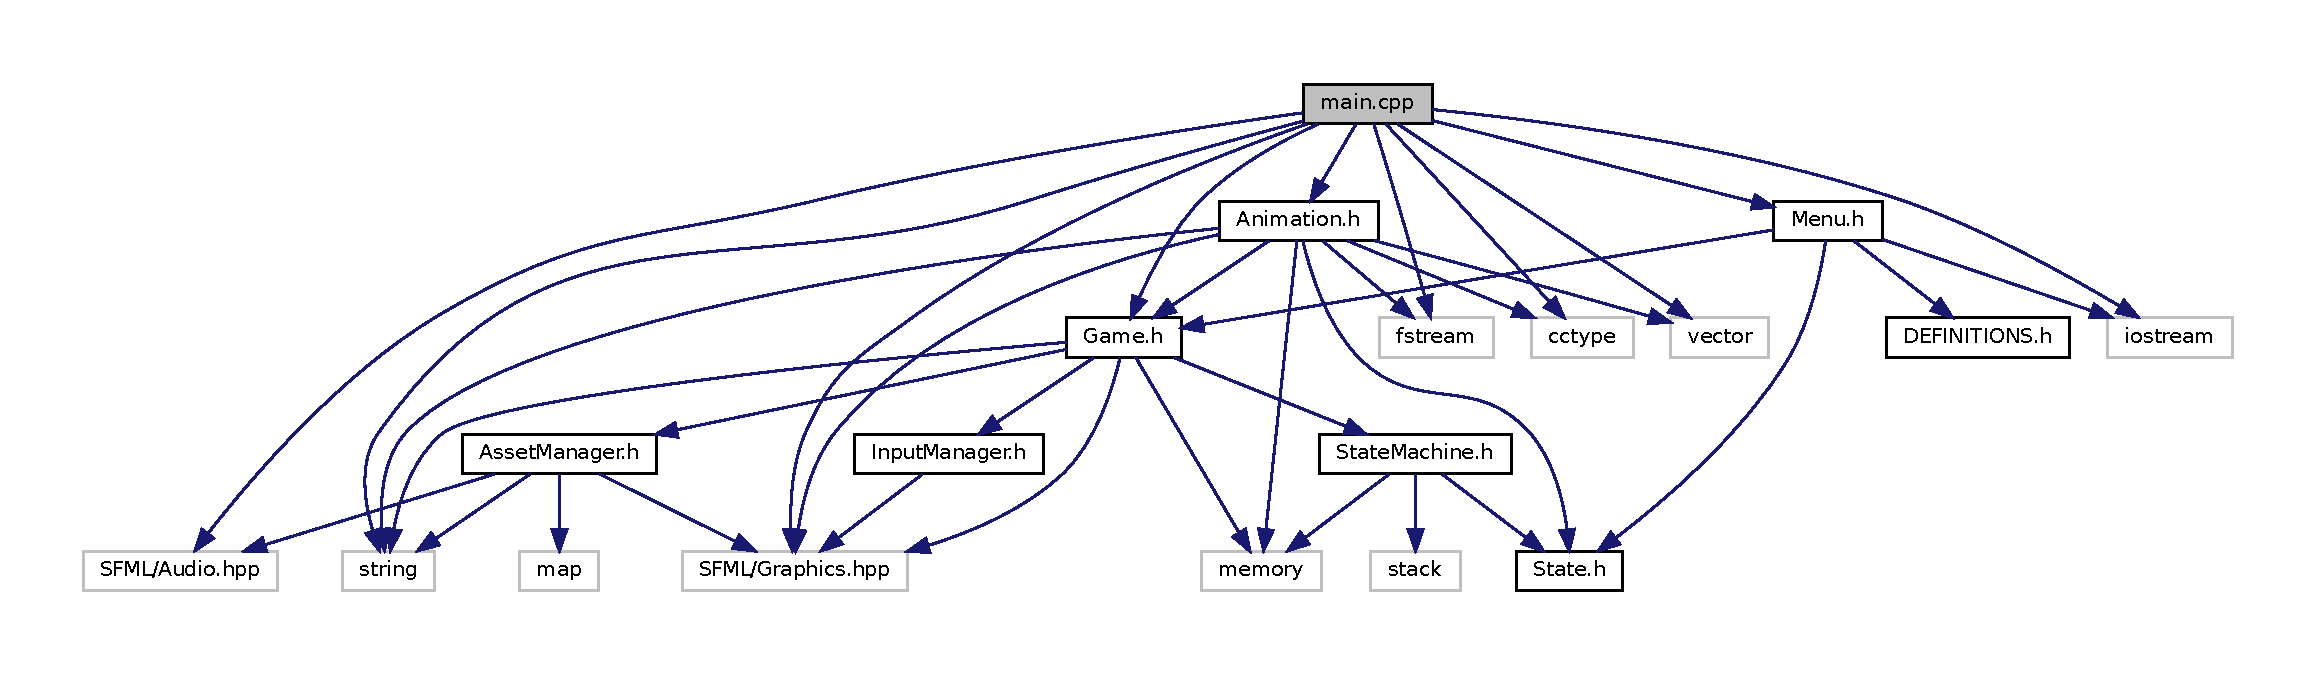
\includegraphics[width=350pt]{main_8cpp__incl}
\end{center}
\end{figure}
\subsection*{Functions}
\begin{DoxyCompactItemize}
\item 
int \mbox{\hyperlink{main_8cpp_ae66f6b31b5ad750f1fe042a706a4e3d4}{main}} ()
\end{DoxyCompactItemize}


\subsection{Function Documentation}
\mbox{\Hypertarget{main_8cpp_ae66f6b31b5ad750f1fe042a706a4e3d4}\label{main_8cpp_ae66f6b31b5ad750f1fe042a706a4e3d4}} 
\index{main.\+cpp@{main.\+cpp}!main@{main}}
\index{main@{main}!main.\+cpp@{main.\+cpp}}
\subsubsection{\texorpdfstring{main()}{main()}}
{\footnotesize\ttfamily int main (\begin{DoxyParamCaption}{ }\end{DoxyParamCaption})}


\hypertarget{Map_8cpp}{}\section{Map.\+cpp File Reference}
\label{Map_8cpp}\index{Map.\+cpp@{Map.\+cpp}}
{\ttfamily \#include \char`\"{}Map.\+h\char`\"{}}\newline
{\ttfamily \#include $<$iostream$>$}\newline
Include dependency graph for Map.\+cpp\+:\nopagebreak
\begin{figure}[H]
\begin{center}
\leavevmode
\includegraphics[width=350pt]{Map_8cpp__incl}
\end{center}
\end{figure}

\hypertarget{Map_8h}{}\section{Map.\+h File Reference}
\label{Map_8h}\index{Map.\+h@{Map.\+h}}
{\ttfamily \#include $<$S\+F\+M\+L/\+Graphics.\+hpp$>$}\newline
{\ttfamily \#include $<$memory$>$}\newline
{\ttfamily \#include \char`\"{}Game.\+h\char`\"{}}\newline
{\ttfamily \#include \char`\"{}State.\+h\char`\"{}}\newline
{\ttfamily \#include \char`\"{}Player.\+h\char`\"{}}\newline
{\ttfamily \#include $<$fstream$>$}\newline
{\ttfamily \#include $<$cctype$>$}\newline
{\ttfamily \#include $<$string$>$}\newline
{\ttfamily \#include $<$vector$>$}\newline
{\ttfamily \#include $<$S\+F\+M\+L/\+Audio.\+hpp$>$}\newline
Include dependency graph for Map.\+h\+:\nopagebreak
\begin{figure}[H]
\begin{center}
\leavevmode
\includegraphics[width=350pt]{Map_8h__incl}
\end{center}
\end{figure}
This graph shows which files directly or indirectly include this file\+:\nopagebreak
\begin{figure}[H]
\begin{center}
\leavevmode
\includegraphics[width=280pt]{Map_8h__dep__incl}
\end{center}
\end{figure}
\subsection*{Classes}
\begin{DoxyCompactItemize}
\item 
struct \mbox{\hyperlink{structTile}{Tile}}
\item 
class \mbox{\hyperlink{classMap}{Map}}
\end{DoxyCompactItemize}

\hypertarget{Menu_8cpp}{}\section{Menu.\+cpp File Reference}
\label{Menu_8cpp}\index{Menu.\+cpp@{Menu.\+cpp}}
{\ttfamily \#include \char`\"{}Menu.\+h\char`\"{}}\newline
{\ttfamily \#include \char`\"{}Stage\+One.\+h\char`\"{}}\newline
Include dependency graph for Menu.\+cpp\+:\nopagebreak
\begin{figure}[H]
\begin{center}
\leavevmode
\includegraphics[width=350pt]{Menu_8cpp__incl}
\end{center}
\end{figure}

\hypertarget{Menu_8h}{}\section{Menu.\+h File Reference}
\label{Menu_8h}\index{Menu.\+h@{Menu.\+h}}
{\ttfamily \#include \char`\"{}D\+E\+F\+I\+N\+I\+T\+I\+O\+N\+S.\+h\char`\"{}}\newline
{\ttfamily \#include \char`\"{}State.\+h\char`\"{}}\newline
{\ttfamily \#include \char`\"{}Game.\+h\char`\"{}}\newline
{\ttfamily \#include $<$iostream$>$}\newline
Include dependency graph for Menu.\+h\+:\nopagebreak
\begin{figure}[H]
\begin{center}
\leavevmode
\includegraphics[width=350pt]{Menu_8h__incl}
\end{center}
\end{figure}
This graph shows which files directly or indirectly include this file\+:\nopagebreak
\begin{figure}[H]
\begin{center}
\leavevmode
\includegraphics[width=350pt]{Menu_8h__dep__incl}
\end{center}
\end{figure}
\subsection*{Classes}
\begin{DoxyCompactItemize}
\item 
class \mbox{\hyperlink{classMenu}{Menu}}
\end{DoxyCompactItemize}

\hypertarget{Player_8cpp}{}\section{Player.\+cpp File Reference}
\label{Player_8cpp}\index{Player.\+cpp@{Player.\+cpp}}
{\ttfamily \#include \char`\"{}Player.\+h\char`\"{}}\newline
{\ttfamily \#include $<$iostream$>$}\newline
{\ttfamily \#include $<$math.\+h$>$}\newline
Include dependency graph for Player.\+cpp\+:\nopagebreak
\begin{figure}[H]
\begin{center}
\leavevmode
\includegraphics[width=350pt]{Player_8cpp__incl}
\end{center}
\end{figure}

\hypertarget{Player_8h}{}\section{Player.\+h File Reference}
\label{Player_8h}\index{Player.\+h@{Player.\+h}}
{\ttfamily \#include $<$S\+F\+M\+L/\+Graphics.\+hpp$>$}\newline
{\ttfamily \#include $<$fstream$>$}\newline
{\ttfamily \#include $<$cctype$>$}\newline
{\ttfamily \#include $<$string$>$}\newline
{\ttfamily \#include $<$vector$>$}\newline
{\ttfamily \#include $<$memory$>$}\newline
{\ttfamily \#include \char`\"{}Animation.\+h\char`\"{}}\newline
{\ttfamily \#include \char`\"{}D\+E\+F\+I\+N\+I\+T\+I\+O\+N\+S.\+h\char`\"{}}\newline
Include dependency graph for Player.\+h\+:\nopagebreak
\begin{figure}[H]
\begin{center}
\leavevmode
\includegraphics[width=350pt]{Player_8h__incl}
\end{center}
\end{figure}
This graph shows which files directly or indirectly include this file\+:\nopagebreak
\begin{figure}[H]
\begin{center}
\leavevmode
\includegraphics[width=286pt]{Player_8h__dep__incl}
\end{center}
\end{figure}
\subsection*{Classes}
\begin{DoxyCompactItemize}
\item 
class \mbox{\hyperlink{classPlayer}{Player}}
\end{DoxyCompactItemize}

\hypertarget{StageOne_8cpp}{}\section{Stage\+One.\+cpp File Reference}
\label{StageOne_8cpp}\index{Stage\+One.\+cpp@{Stage\+One.\+cpp}}
{\ttfamily \#include \char`\"{}Stage\+One.\+h\char`\"{}}\newline
{\ttfamily \#include $<$iostream$>$}\newline
Include dependency graph for Stage\+One.\+cpp\+:\nopagebreak
\begin{figure}[H]
\begin{center}
\leavevmode
\includegraphics[width=350pt]{StageOne_8cpp__incl}
\end{center}
\end{figure}

\hypertarget{StageOne_8h}{}\section{Stage\+One.\+h File Reference}
\label{StageOne_8h}\index{Stage\+One.\+h@{Stage\+One.\+h}}
{\ttfamily \#include $<$S\+F\+M\+L/\+Graphics.\+hpp$>$}\newline
{\ttfamily \#include $<$S\+F\+M\+L/\+Audio.\+hpp$>$}\newline
{\ttfamily \#include \char`\"{}D\+E\+F\+I\+N\+I\+T\+I\+O\+N\+S.\+h\char`\"{}}\newline
{\ttfamily \#include \char`\"{}State.\+h\char`\"{}}\newline
{\ttfamily \#include \char`\"{}Game.\+h\char`\"{}}\newline
{\ttfamily \#include \char`\"{}Map.\+h\char`\"{}}\newline
{\ttfamily \#include $<$memory$>$}\newline
{\ttfamily \#include $<$vector$>$}\newline
{\ttfamily \#include \char`\"{}Player.\+h\char`\"{}}\newline
{\ttfamily \#include \char`\"{}Game\+Over.\+h\char`\"{}}\newline
Include dependency graph for Stage\+One.\+h\+:\nopagebreak
\begin{figure}[H]
\begin{center}
\leavevmode
\includegraphics[width=350pt]{StageOne_8h__incl}
\end{center}
\end{figure}
This graph shows which files directly or indirectly include this file\+:\nopagebreak
\begin{figure}[H]
\begin{center}
\leavevmode
\includegraphics[width=246pt]{StageOne_8h__dep__incl}
\end{center}
\end{figure}
\subsection*{Classes}
\begin{DoxyCompactItemize}
\item 
class \mbox{\hyperlink{classStageOne}{Stage\+One}}
\end{DoxyCompactItemize}

\hypertarget{State_8h}{}\section{State.\+h File Reference}
\label{State_8h}\index{State.\+h@{State.\+h}}
This graph shows which files directly or indirectly include this file\+:\nopagebreak
\begin{figure}[H]
\begin{center}
\leavevmode
\includegraphics[width=350pt]{State_8h__dep__incl}
\end{center}
\end{figure}
\subsection*{Classes}
\begin{DoxyCompactItemize}
\item 
class \mbox{\hyperlink{classState}{State}}
\end{DoxyCompactItemize}

\hypertarget{StateMachine_8cpp}{}\section{State\+Machine.\+cpp File Reference}
\label{StateMachine_8cpp}\index{State\+Machine.\+cpp@{State\+Machine.\+cpp}}
{\ttfamily \#include \char`\"{}State\+Machine.\+h\char`\"{}}\newline
{\ttfamily \#include $<$iostream$>$}\newline
Include dependency graph for State\+Machine.\+cpp\+:\nopagebreak
\begin{figure}[H]
\begin{center}
\leavevmode
\includegraphics[width=302pt]{StateMachine_8cpp__incl}
\end{center}
\end{figure}

\hypertarget{StateMachine_8h}{}\section{State\+Machine.\+h File Reference}
\label{StateMachine_8h}\index{State\+Machine.\+h@{State\+Machine.\+h}}
{\ttfamily \#include $<$memory$>$}\newline
{\ttfamily \#include $<$stack$>$}\newline
{\ttfamily \#include \char`\"{}State.\+h\char`\"{}}\newline
Include dependency graph for State\+Machine.\+h\+:\nopagebreak
\begin{figure}[H]
\begin{center}
\leavevmode
\includegraphics[width=269pt]{StateMachine_8h__incl}
\end{center}
\end{figure}
This graph shows which files directly or indirectly include this file\+:\nopagebreak
\begin{figure}[H]
\begin{center}
\leavevmode
\includegraphics[width=350pt]{StateMachine_8h__dep__incl}
\end{center}
\end{figure}
\subsection*{Classes}
\begin{DoxyCompactItemize}
\item 
class \mbox{\hyperlink{classStateMachine}{State\+Machine}}
\end{DoxyCompactItemize}
\subsection*{Typedefs}
\begin{DoxyCompactItemize}
\item 
using \mbox{\hyperlink{StateMachine_8h_a217d9c9b187e9dd27abb46be48fb014d}{State\+Ref}} = std\+::unique\+\_\+ptr$<$ \mbox{\hyperlink{classState}{State}} $>$
\end{DoxyCompactItemize}


\subsection{Typedef Documentation}
\mbox{\Hypertarget{StateMachine_8h_a217d9c9b187e9dd27abb46be48fb014d}\label{StateMachine_8h_a217d9c9b187e9dd27abb46be48fb014d}} 
\index{State\+Machine.\+h@{State\+Machine.\+h}!State\+Ref@{State\+Ref}}
\index{State\+Ref@{State\+Ref}!State\+Machine.\+h@{State\+Machine.\+h}}
\subsubsection{\texorpdfstring{State\+Ref}{StateRef}}
{\footnotesize\ttfamily using \mbox{\hyperlink{StateMachine_8h_a217d9c9b187e9dd27abb46be48fb014d}{State\+Ref}} =  std\+::unique\+\_\+ptr$<$\mbox{\hyperlink{classState}{State}}$>$}

Pointer to every state, named State\+Ref 
%--- End generated contents ---

% Index
\backmatter
\newpage
\phantomsection
\clearemptydoublepage
\addcontentsline{toc}{chapter}{Index}
\printindex

\end{document}
